\documentclass{beamer}

\usepackage{graphicx}
\usepackage{mwe}

%%%%%%%%%%%%%%%%%%%%%%%%%%%%%%%%%%%%%%%%%%%%%%%%%%%%%%%%%%%%%%%%%%%%%%%%%%%%%%%%
%
%  \zoombox[box line width]{contents}
%
%  optimized version for beamer: in full screen, zoom boxes are centred
%  in the viewer; useable with any documenclass
%
%%%%%%%%%%%%%%%%%%%%%%%%%%%%%%%%%%%%%%%%%%%%%%%%%%%%%%%%%%%%%%%%%%%%%%%%%%%%%%%%
\makeatletter
\newsavebox\zb@x
\newcounter{z@@m}
\usepackage{calc}
\newdimen\B@r\newdimen\P@r
\newdimen\@zw\newdimen\@zh\newdimen\@zd

\newcommand{\zoombox}[2][0]{%
  \leavevmode%
  \sbox\zb@x{#2}%
  \setlength\B@r{1pt*\ratio{\wd\zb@x}{\ht\zb@x+\dp\zb@x}}%
  \setlength\P@r{1pt*\ratio{\paperwidth}{\paperheight}}%
  \ifdim\B@r>\P@r\relax%
    \setlength\@zw{\wd\zb@x}\setlength\@zh{\@zw*\ratio{\paperheight}{\paperwidth}}%
    \setlength\@zd{(\@zh-\ht\zb@x-\dp\zb@x)*\real{0.5}+\dp\zb@x}%
    \setlength\@zh{\@zh-\@zd}%
  \else%
    \setlength\@zh{\ht\zb@x+\dp\zb@x}%
    \setlength\@zw{\@zh*\ratio{\paperwidth}{\paperheight}}%
    \setlength\@zh{\ht\zb@x}\setlength\@zd{\dp\zb@x}%
  \fi%
  \makebox[0pt][l]{\makebox[\wd\zb@x][c]{\makebox[\@zw][l]{%
    \pdfdest name {zbfs\thez@@m} fitr
      width  \@zw\space
      height \@zh\space
      depth  \@zd\space
  }}}%
  \pdfdest name {zb\thez@@m} fitr
    width  \wd\zb@x\space
    height \ht\zb@x\space
    depth  \dp\zb@x\space
  \immediate\pdfannot 
    width  \wd\zb@x\space
    height \ht\zb@x\space
    depth  \dp\zb@x\space
  {%
    /Subtype/Link/H/N
    /Border [0 0 #1 [1 2]]
    /A <<
      /S/JavaScript
      /JS (
        if(typeof(zoomed)=='undefined'||!zoomed){
          var lastView=this.viewState;
          if(app.fs.isFullScreen) this.gotoNamedDest('zbfs\thez@@m');
          else this.gotoNamedDest('zb\thez@@m');
          zoomed=true;
        }else{
          this.viewState=lastView;
          zoomed=false;
        }
      )
    >>
  }%
  \usebox{\zb@x}%
  \stepcounter{z@@m}%
} 
\makeatother
%%%%%%%%%%%%%%%%%%%%%%%%%%%%%%%%%%%%%%%%%%%%%%%%%%%%%%%%%%%%%%%%%%%%%%%%%%%%%%%


\title{HandsOn-SEA Build Guide}  \vspace{25mm}
\date{}

\begin{document}
\setbeamertemplate{caption}{\raggedright\insertcaption\par} %To remove "Figure:" from caption
\begin{frame}[t, plain]
  \vspace{15mm}
  \titlepage
  \vspace{0mm}
*All the pictures placed on the document can be zoomed in an out by click on them. You may need Adobe Acrobat for this functionality. \\
*Selection of different motors can necessitate some minor changes in the designs  of certain parts but they don't affect the manufacturing procedure. 
\end{frame}

\begin{frame}[t]{Assembling the base}
\begin{itemize} 
\item Components
\begin{itemize} \scriptsize
\setlength\itemsep{0.5mm}
\item Plexiglass base (Base)
\item Plexiglass base (Side)
\item Plexiglass base (Face)
\item Bearing
\item Plexiglass base (Lower plate)(Optional)
\item Super glue 
\item Cloroform (Optional)
\end{itemize}

\item Procedure
\begin{enumerate} \scriptsize
\item Glue one of the sides parts and face part together.
\item Glue the other face part to the assembly.
\item Glue the assembly into the plexiglass base.
\item Glue the bearing into the face.
\item Use glue or cloroform to fix the base assembly on the lower plate (Optional)
\end{enumerate}
\end{itemize}
\vspace{-1mm}
\scriptsize End product of this section should look like:
\newline
\zoombox{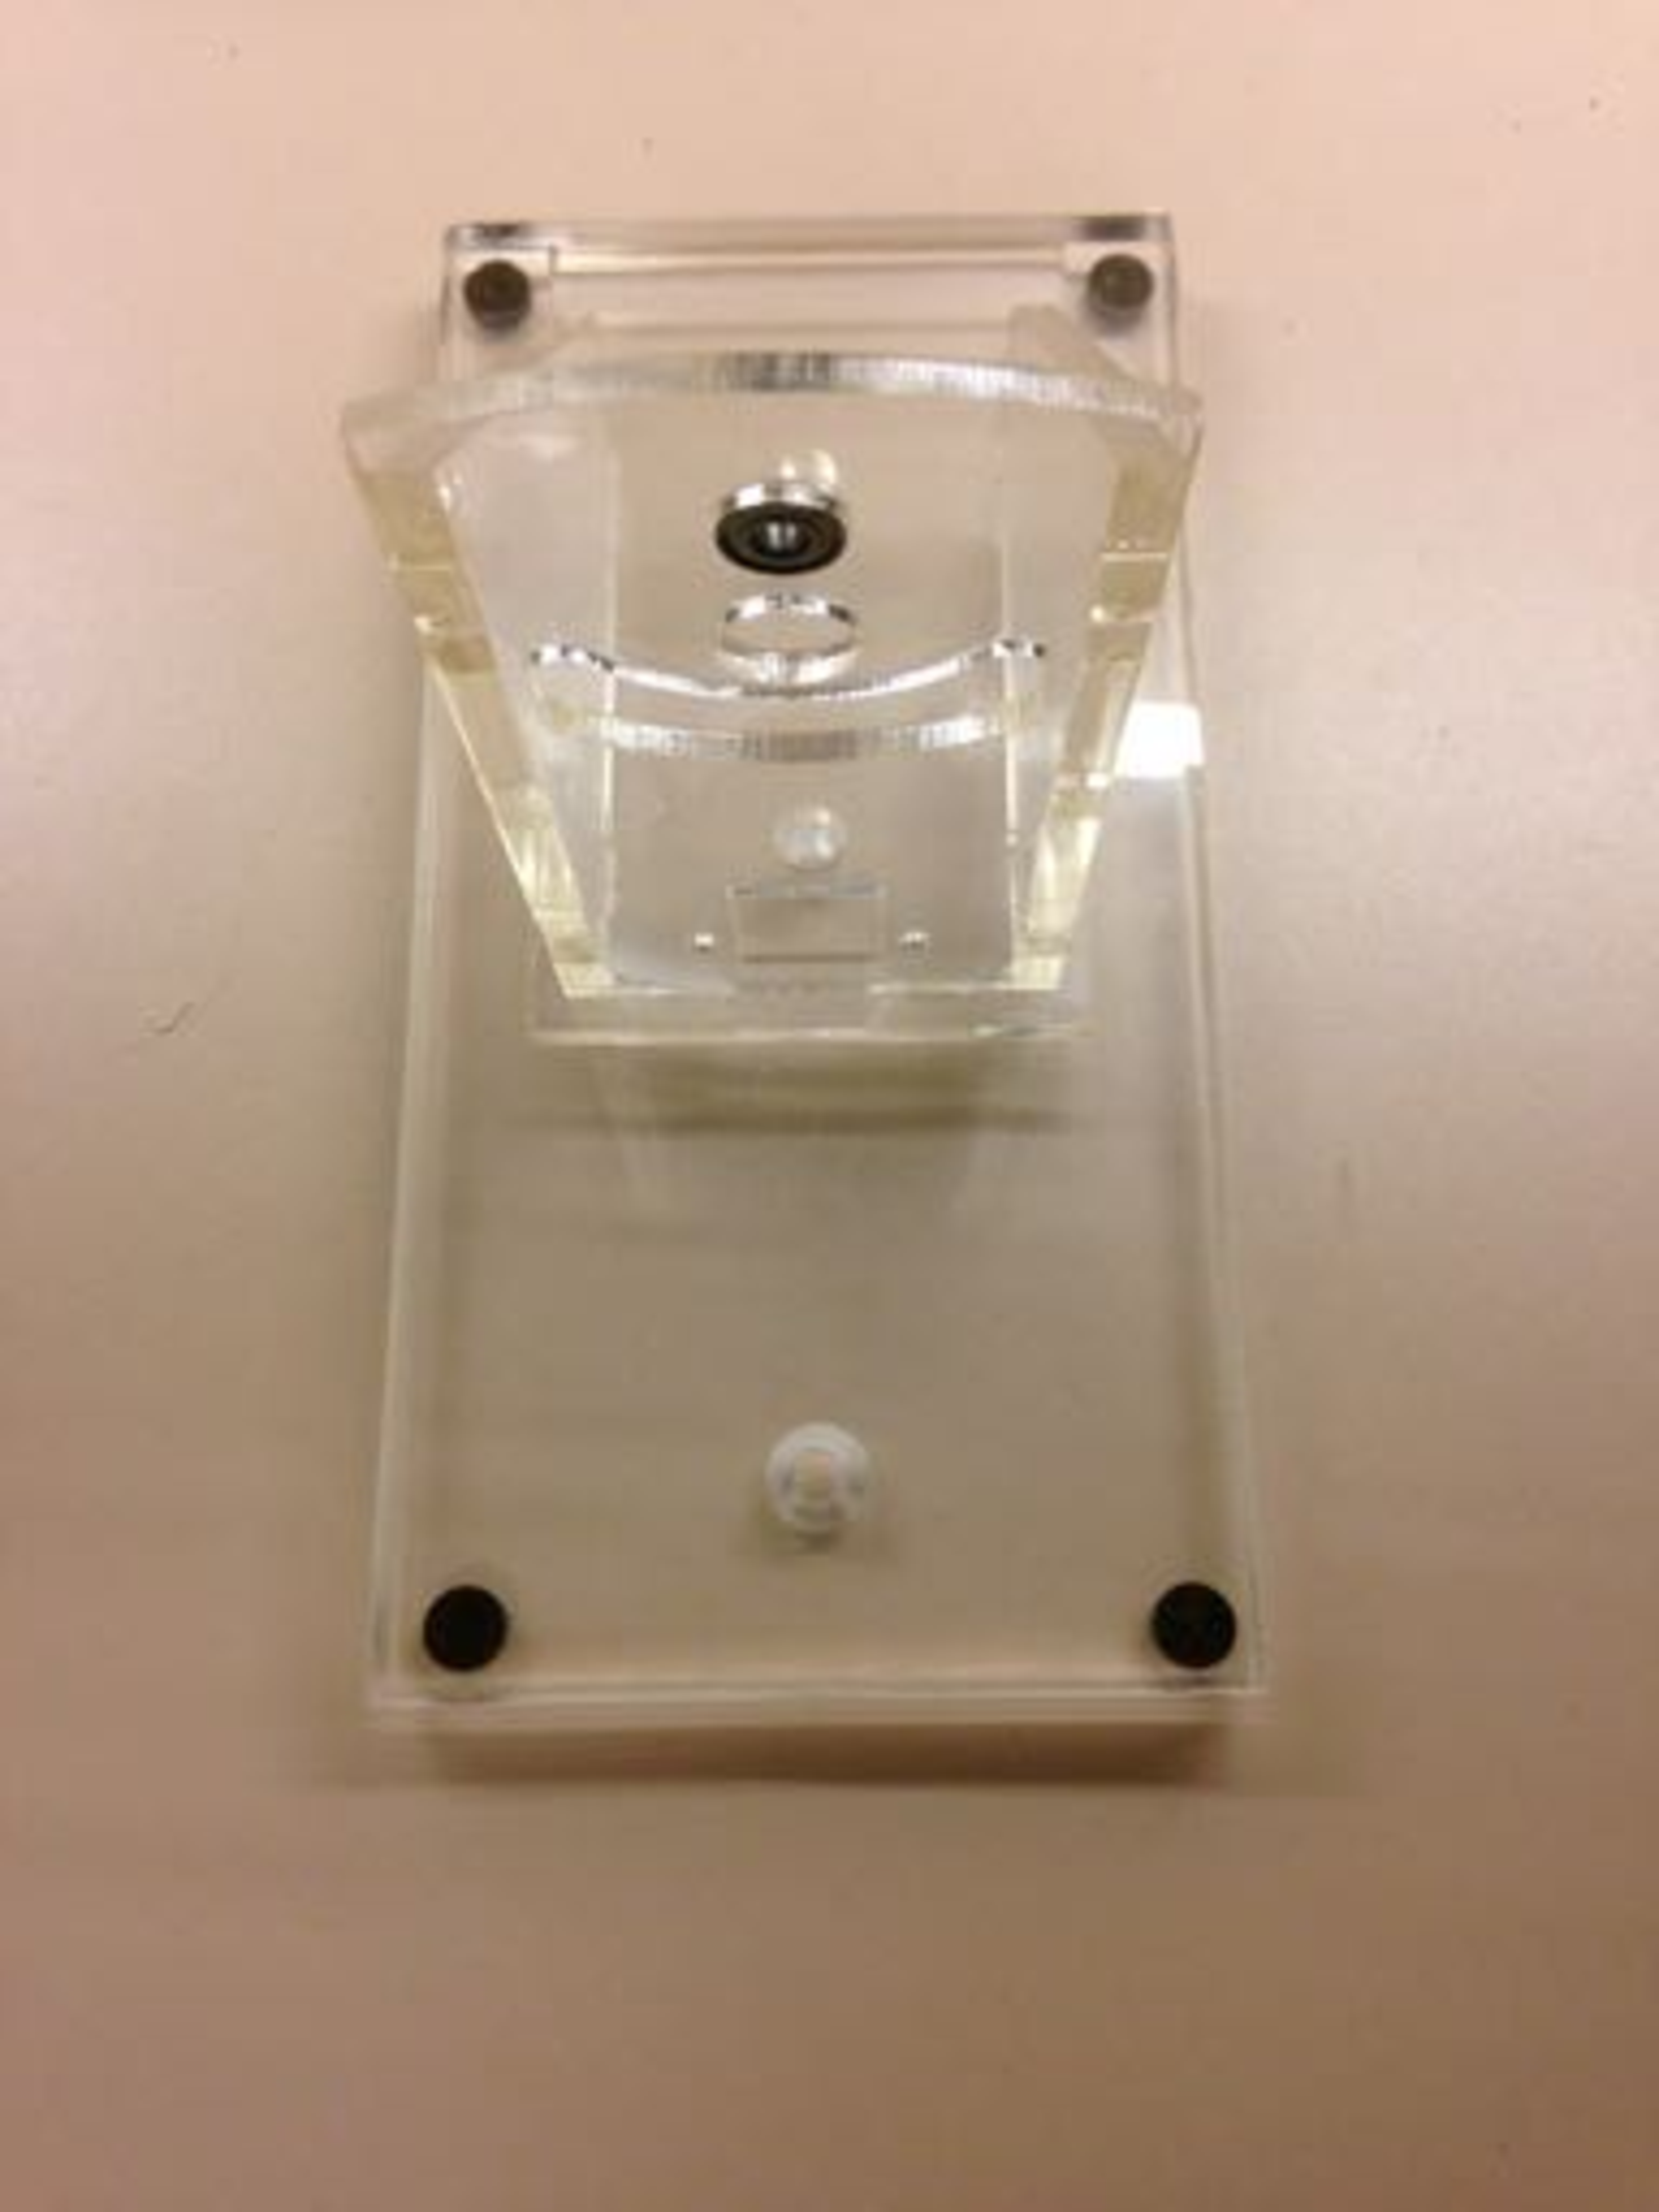
\includegraphics[width=1cm]{./figures/base_front.pdf}}
\zoombox{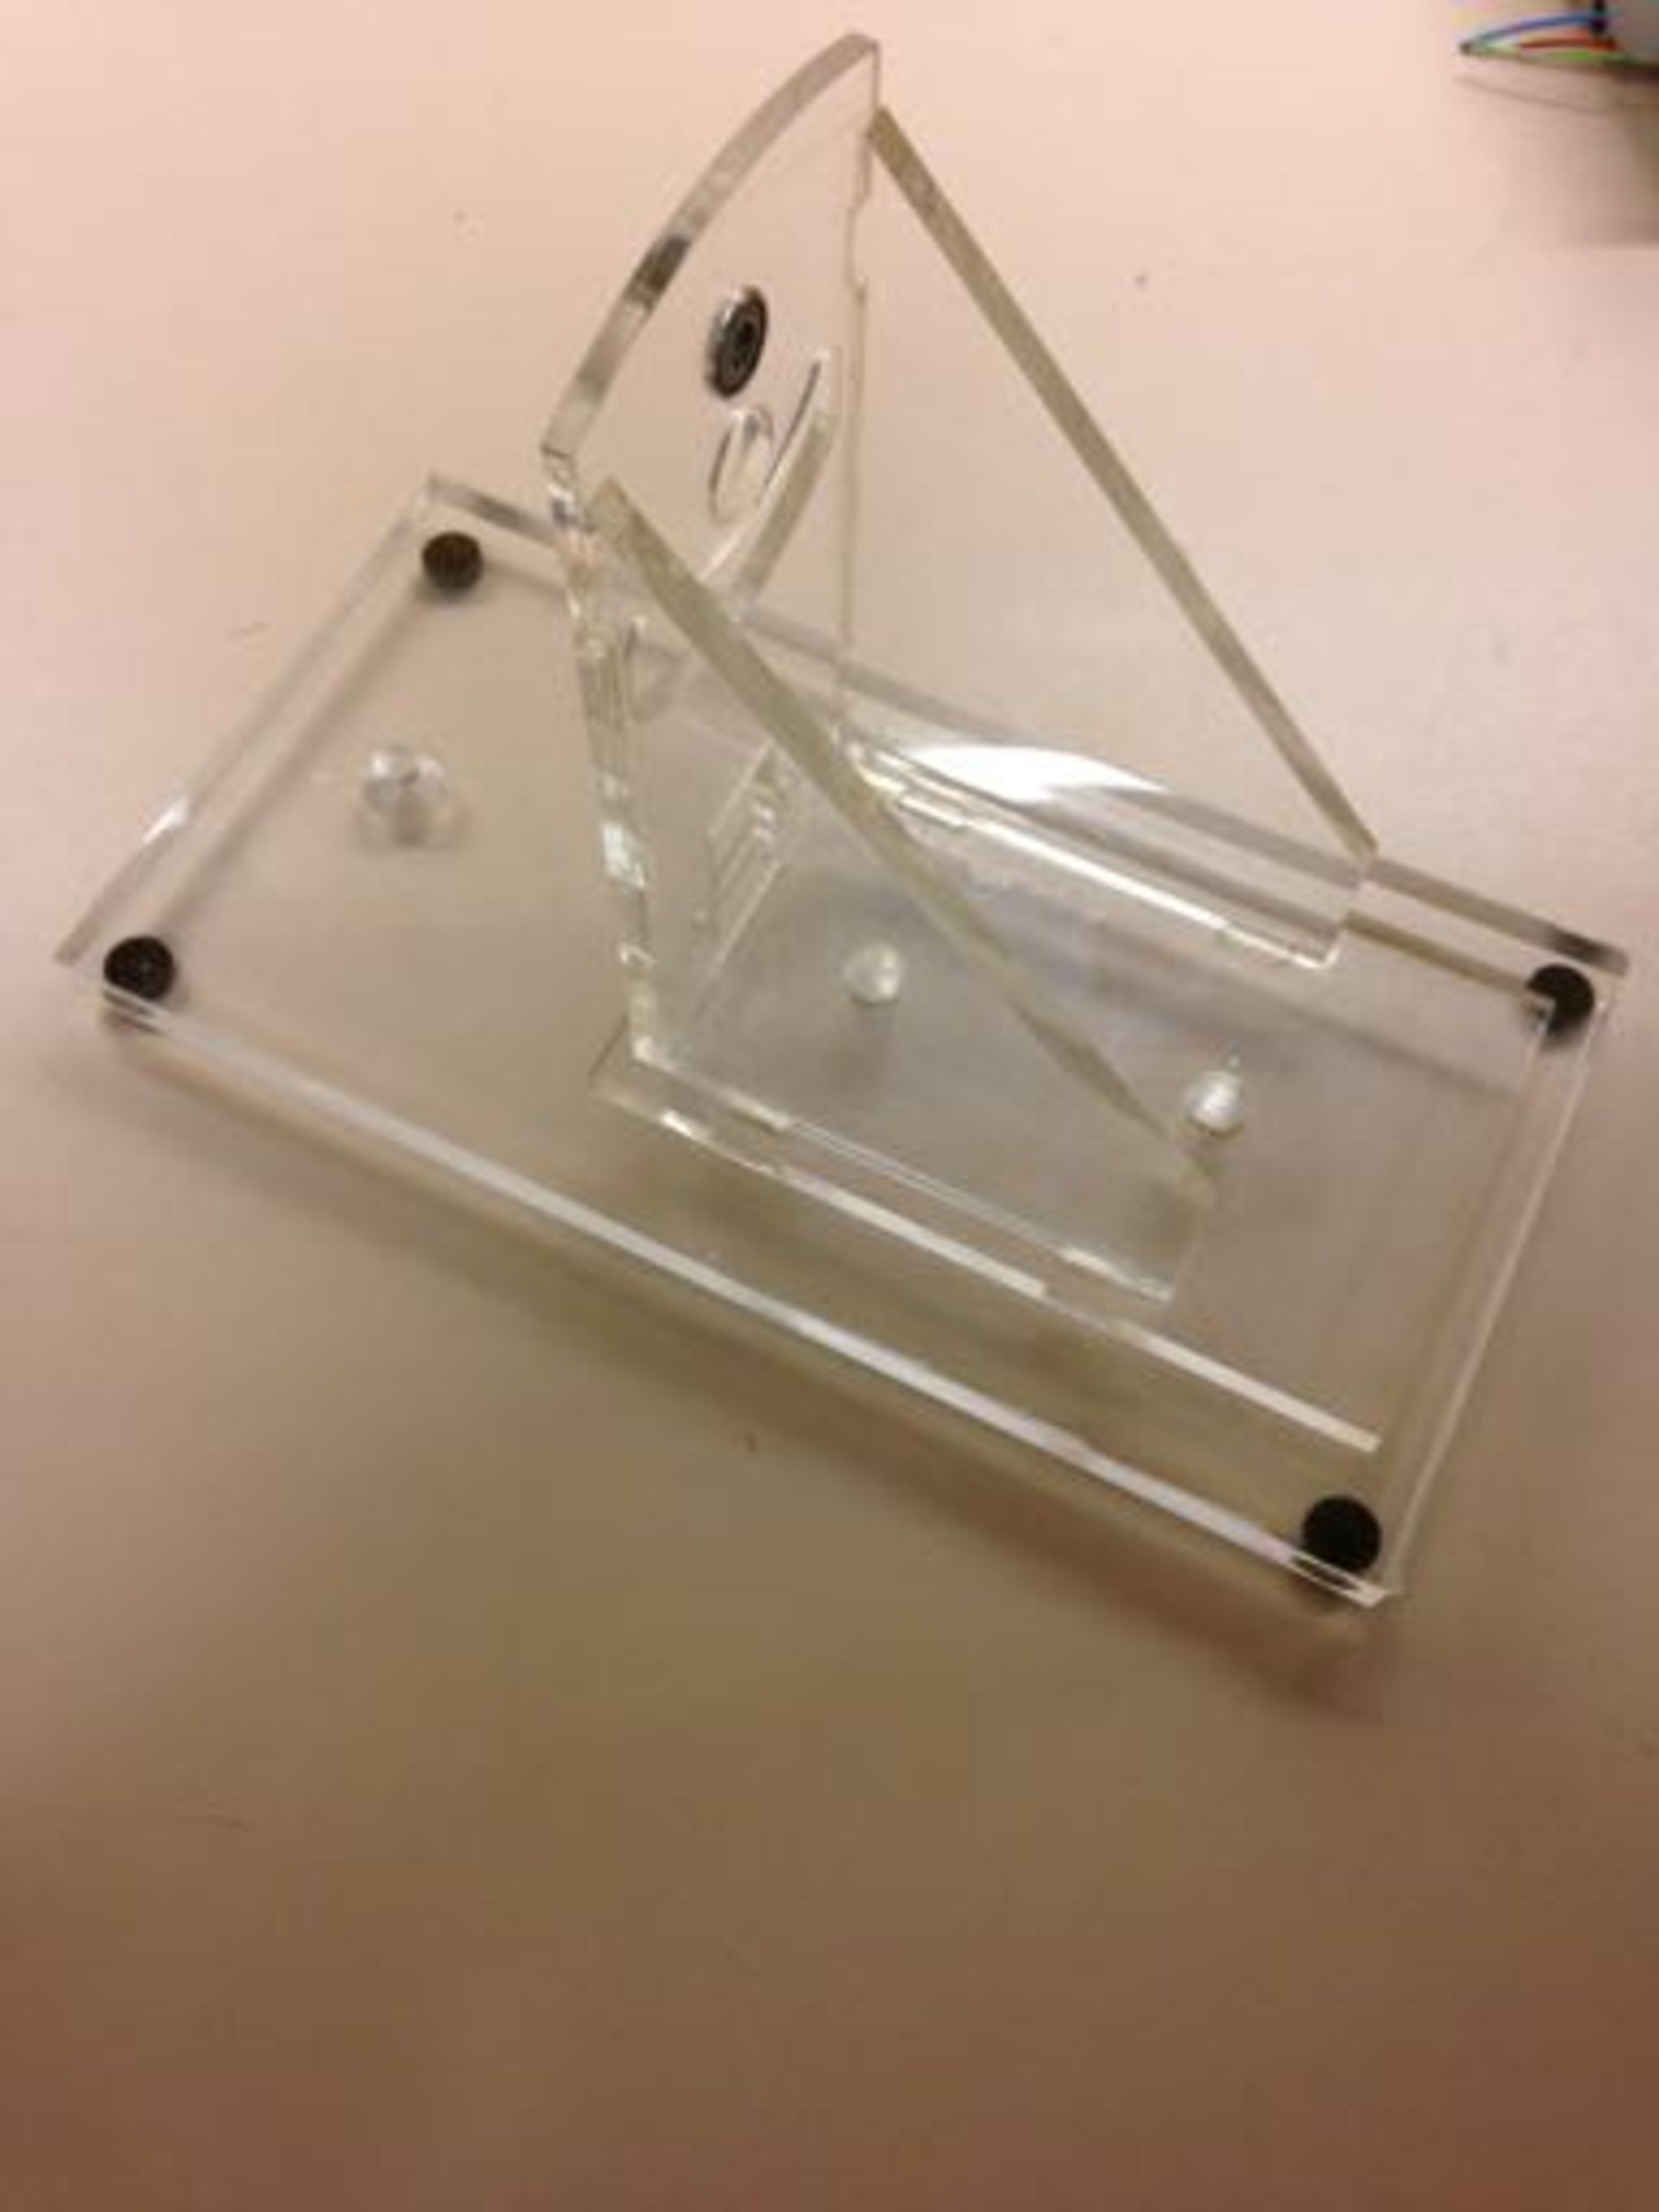
\includegraphics[width=1cm]{./figures/base_diag.pdf}}
\zoombox{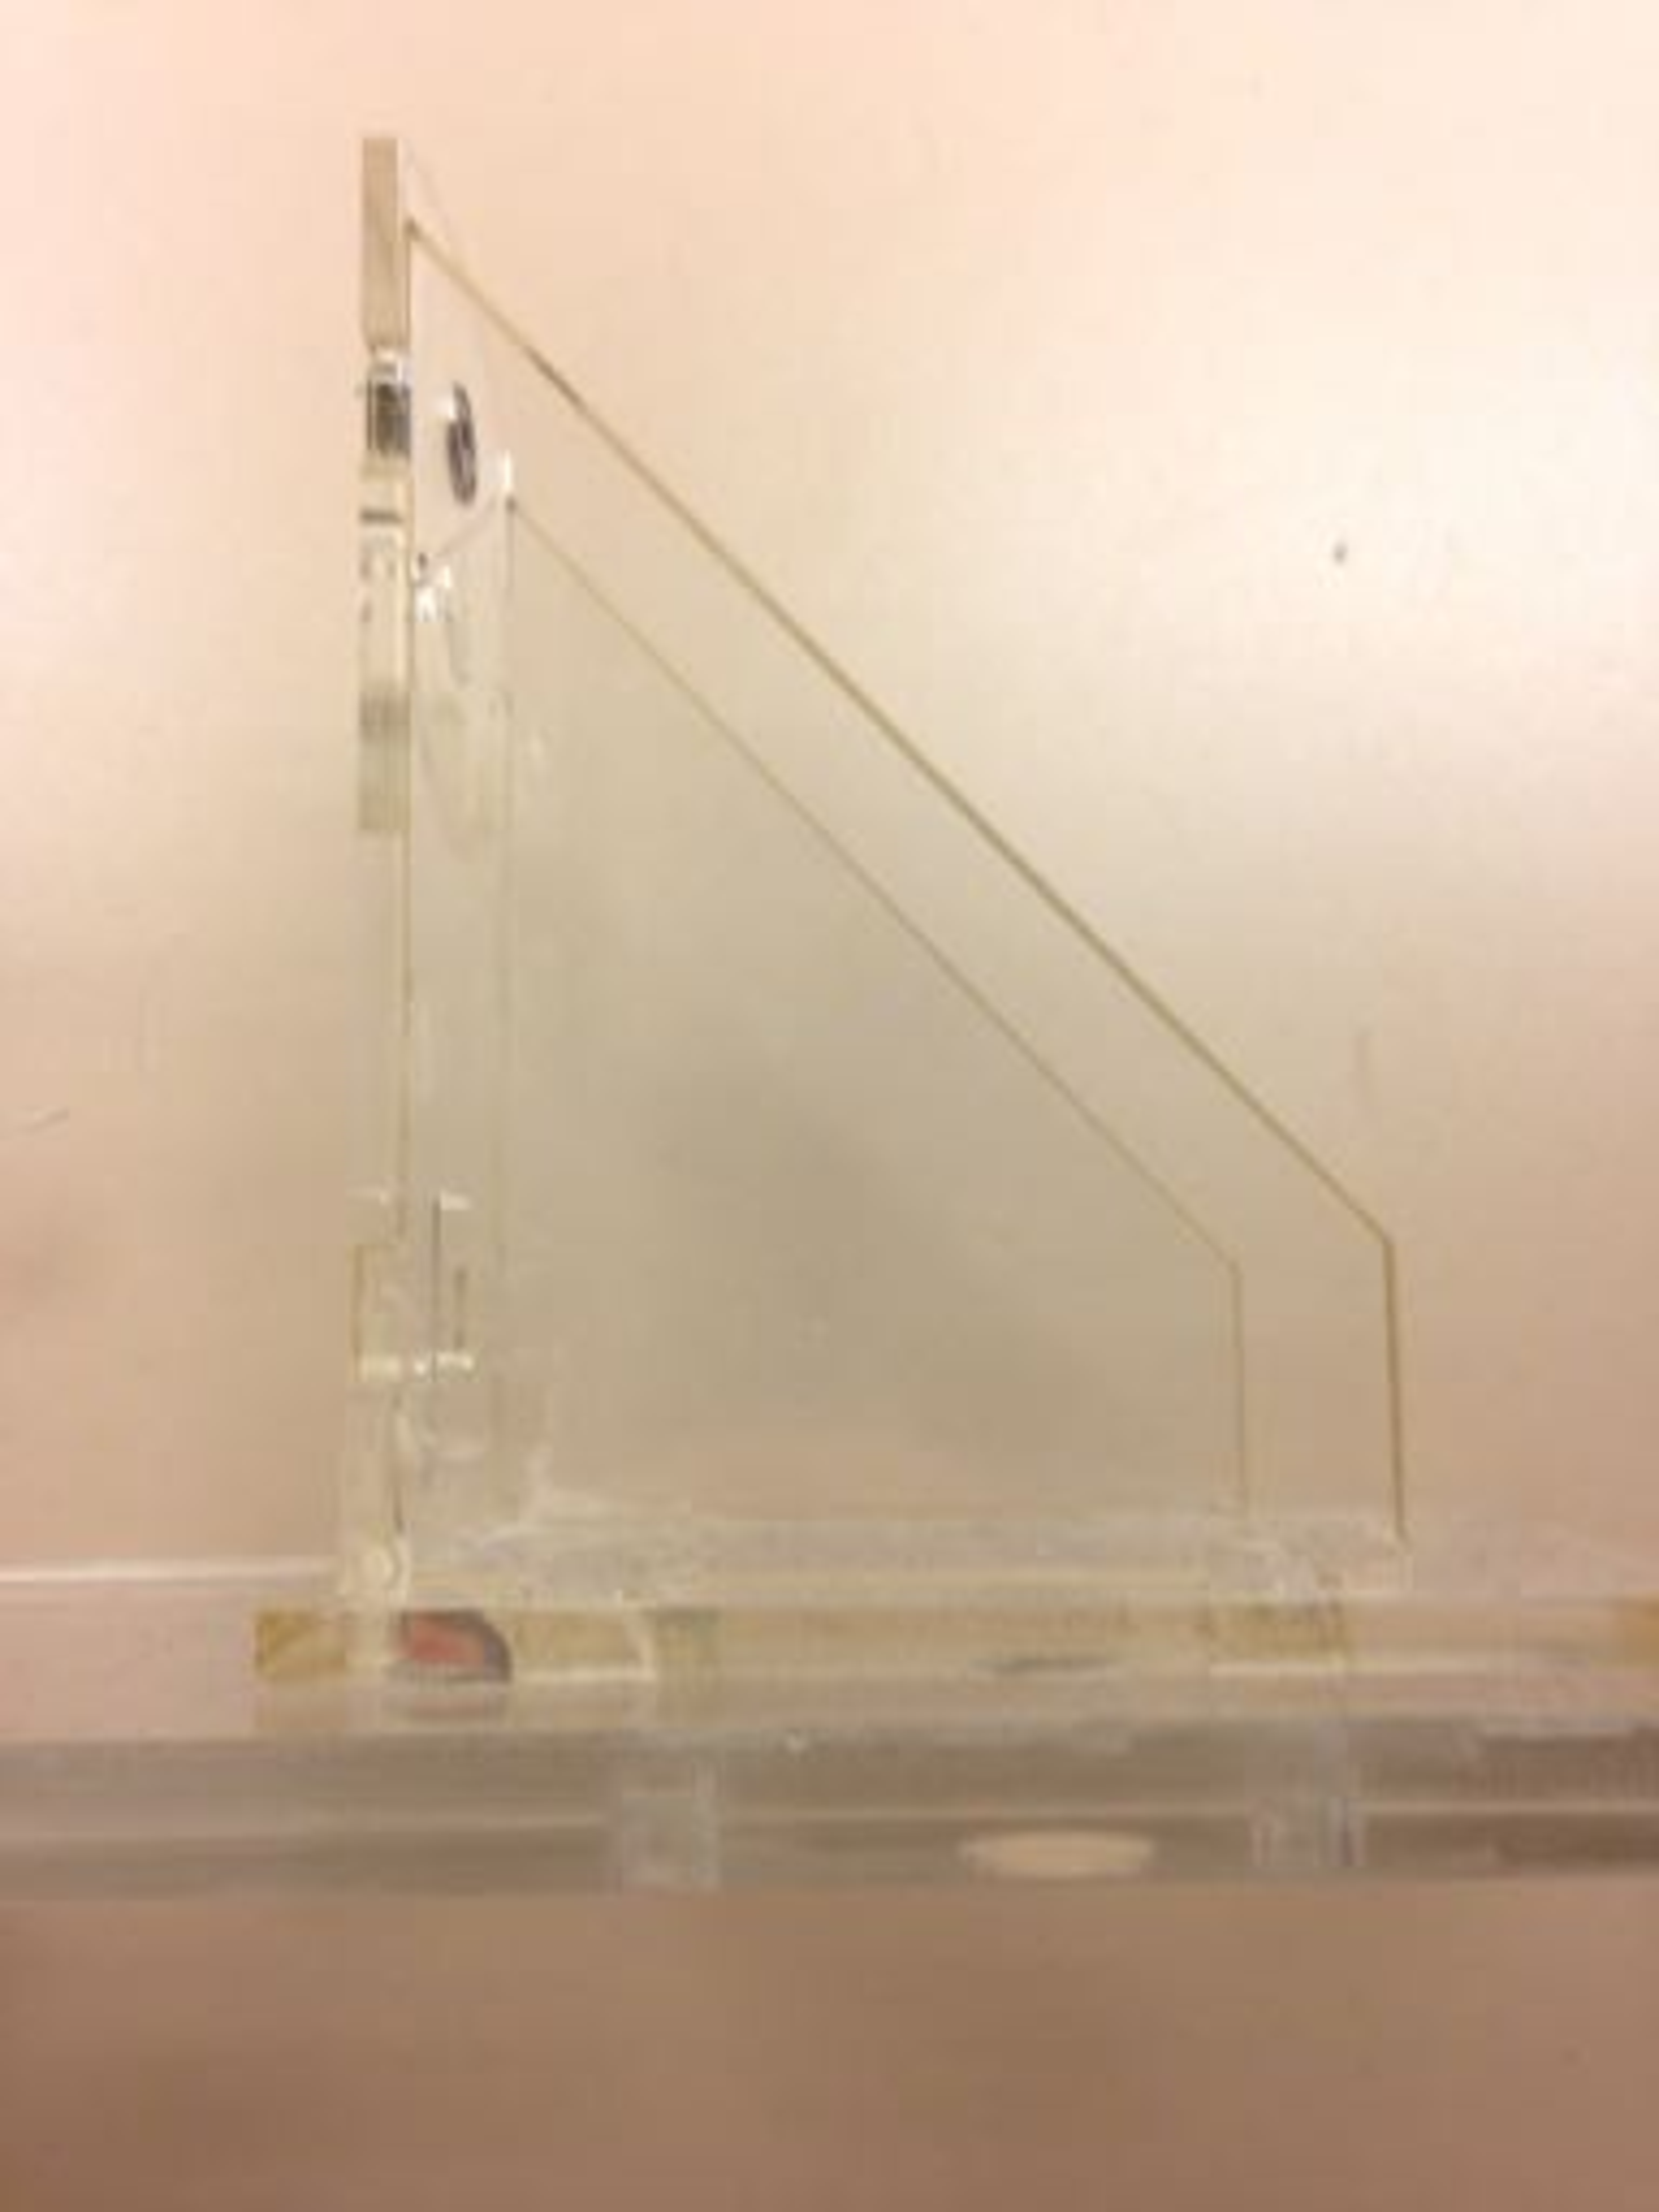
\includegraphics[width=1cm]{./figures/base_right.pdf}}
\end{frame}


\begin{frame}[t]{Assembling the Handle, Pulley and spring steels}
\vspace{-2mm}
\begin{itemize}
\item	Components
\newline
\begin{minipage}{0.4\textwidth} 
\raggedright
\begin{itemize} \scriptsize
\setlength\itemsep{-0.3mm}
\item	3D printed pulley
\item	3D printed handle
\item	4x spring steels
\item Hall effect sensor
\item 3 pin single row pin header
\end{itemize}
\end{minipage}
\begin{minipage}{0.5\textwidth}
\begin{itemize} \scriptsize
\setlength\itemsep{-0.5mm}
\item 8x screws(D:2 mm, L: 15mm)
\item 8x screws(D:2 mm, L: 10mm)
\item 16x 2mm nuts and washers
\item Screw driver
\item Tooth pick
\item Positioning base
\end{itemize}
\end{minipage}
\vspace{1mm}
\item Procedure 
\begin{enumerate} \scriptsize
\item First take out the metal pieces and then glue the 3 pin female header on the handle.
\item Mount the hall effect sensor into the handle.
\zoombox{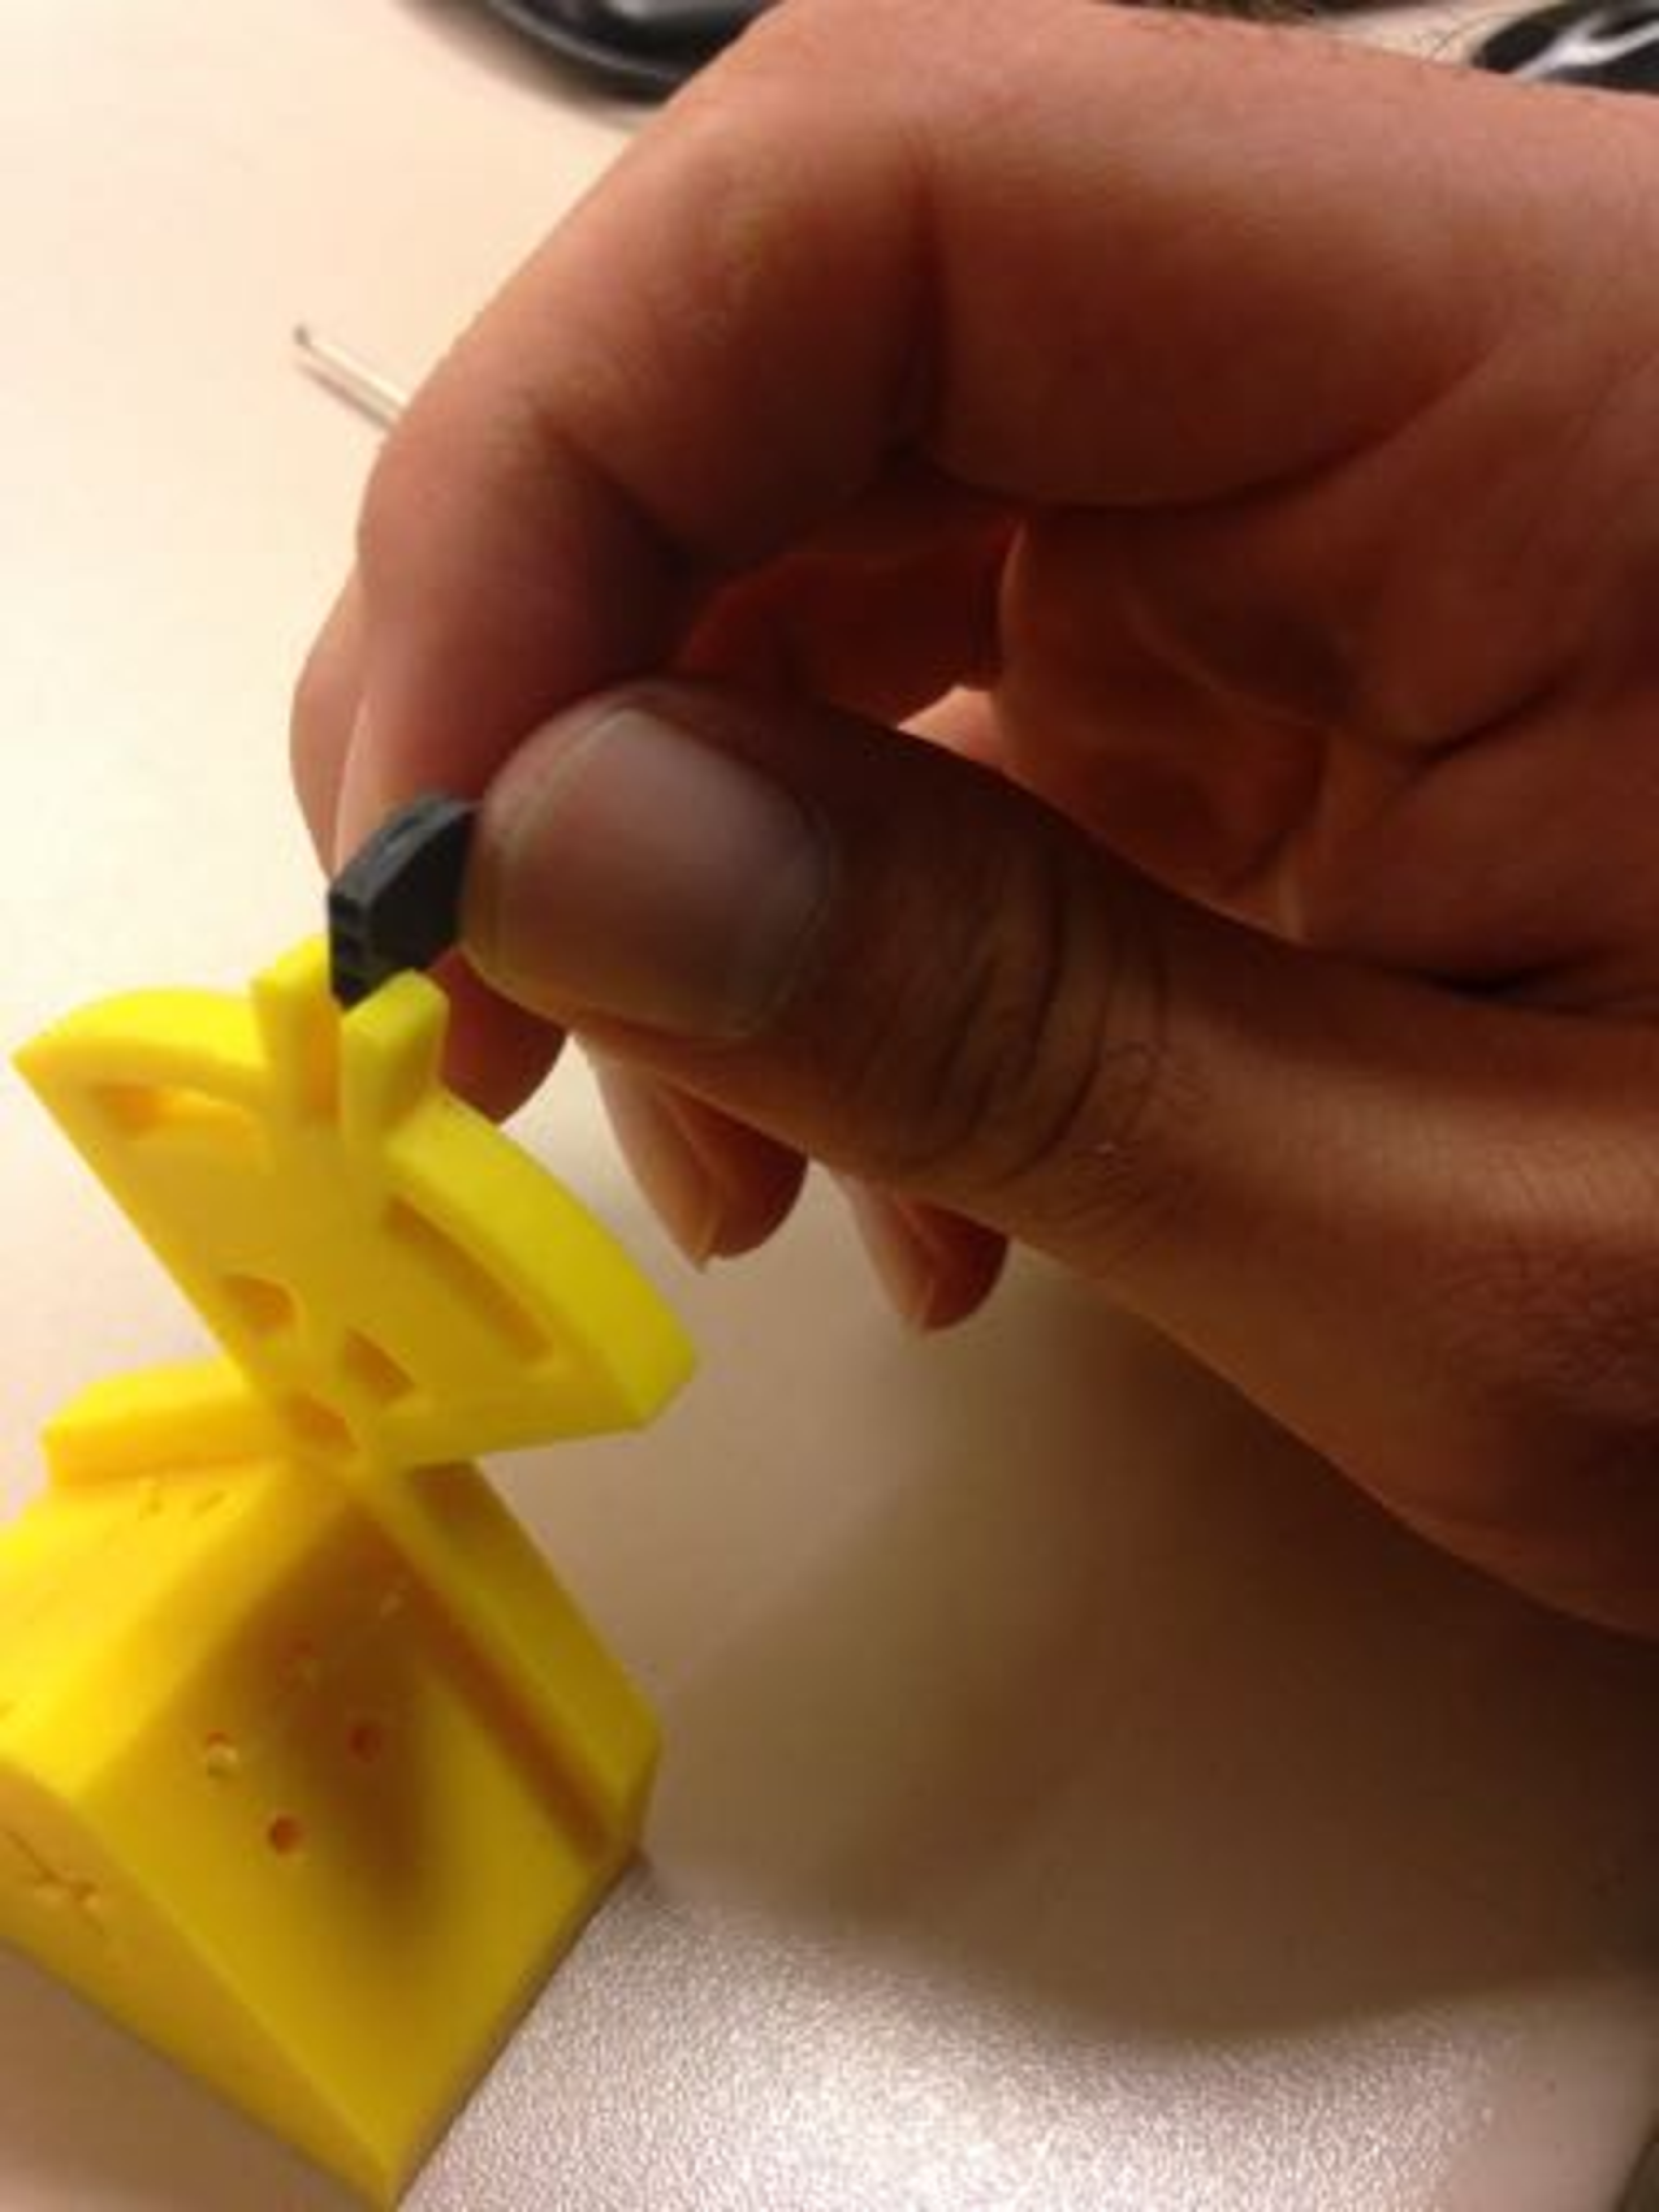
\includegraphics[width=3mm]{./figures/sensor_mount.pdf}}
\item Solder the legs of the hall effect sensor with cables, use heat shrink tubes and hot glue gun to protect the legs. 
\item Mount the cube magnets into the pulley with each magnet facing the same pole towards each other
\zoombox{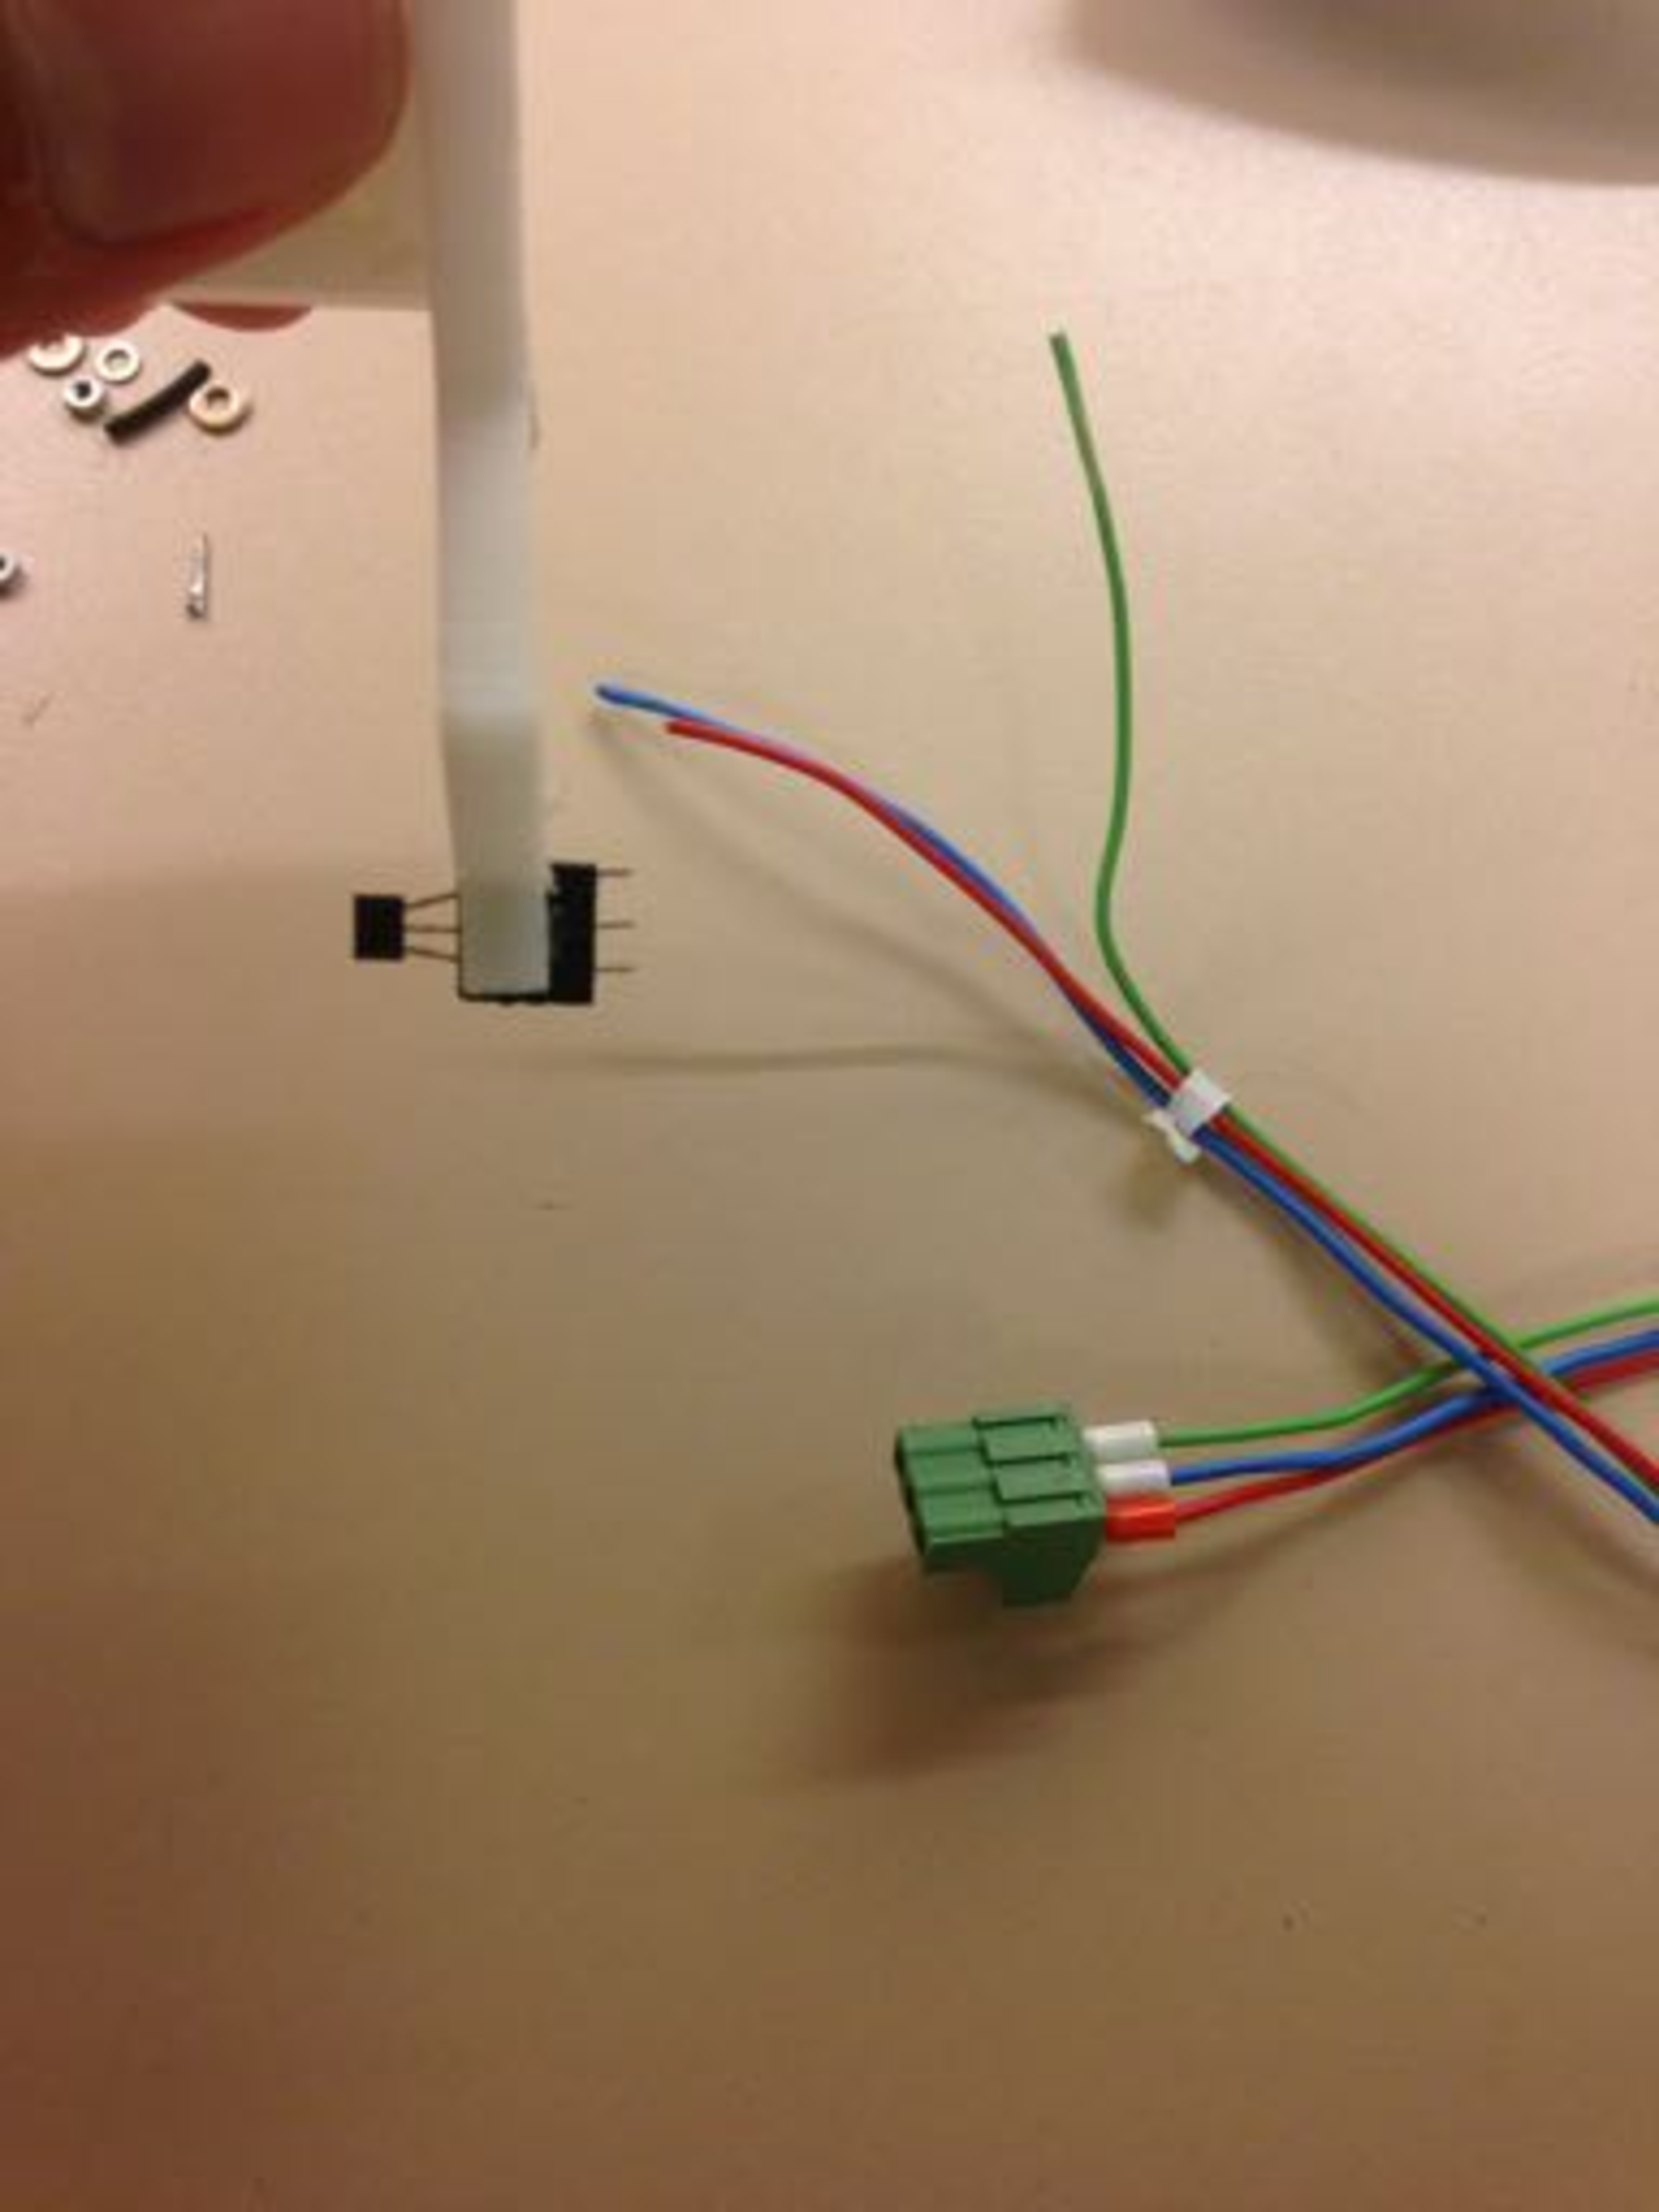
\includegraphics[width=3mm]{./figures/sensor_solder.pdf}}
\zoombox{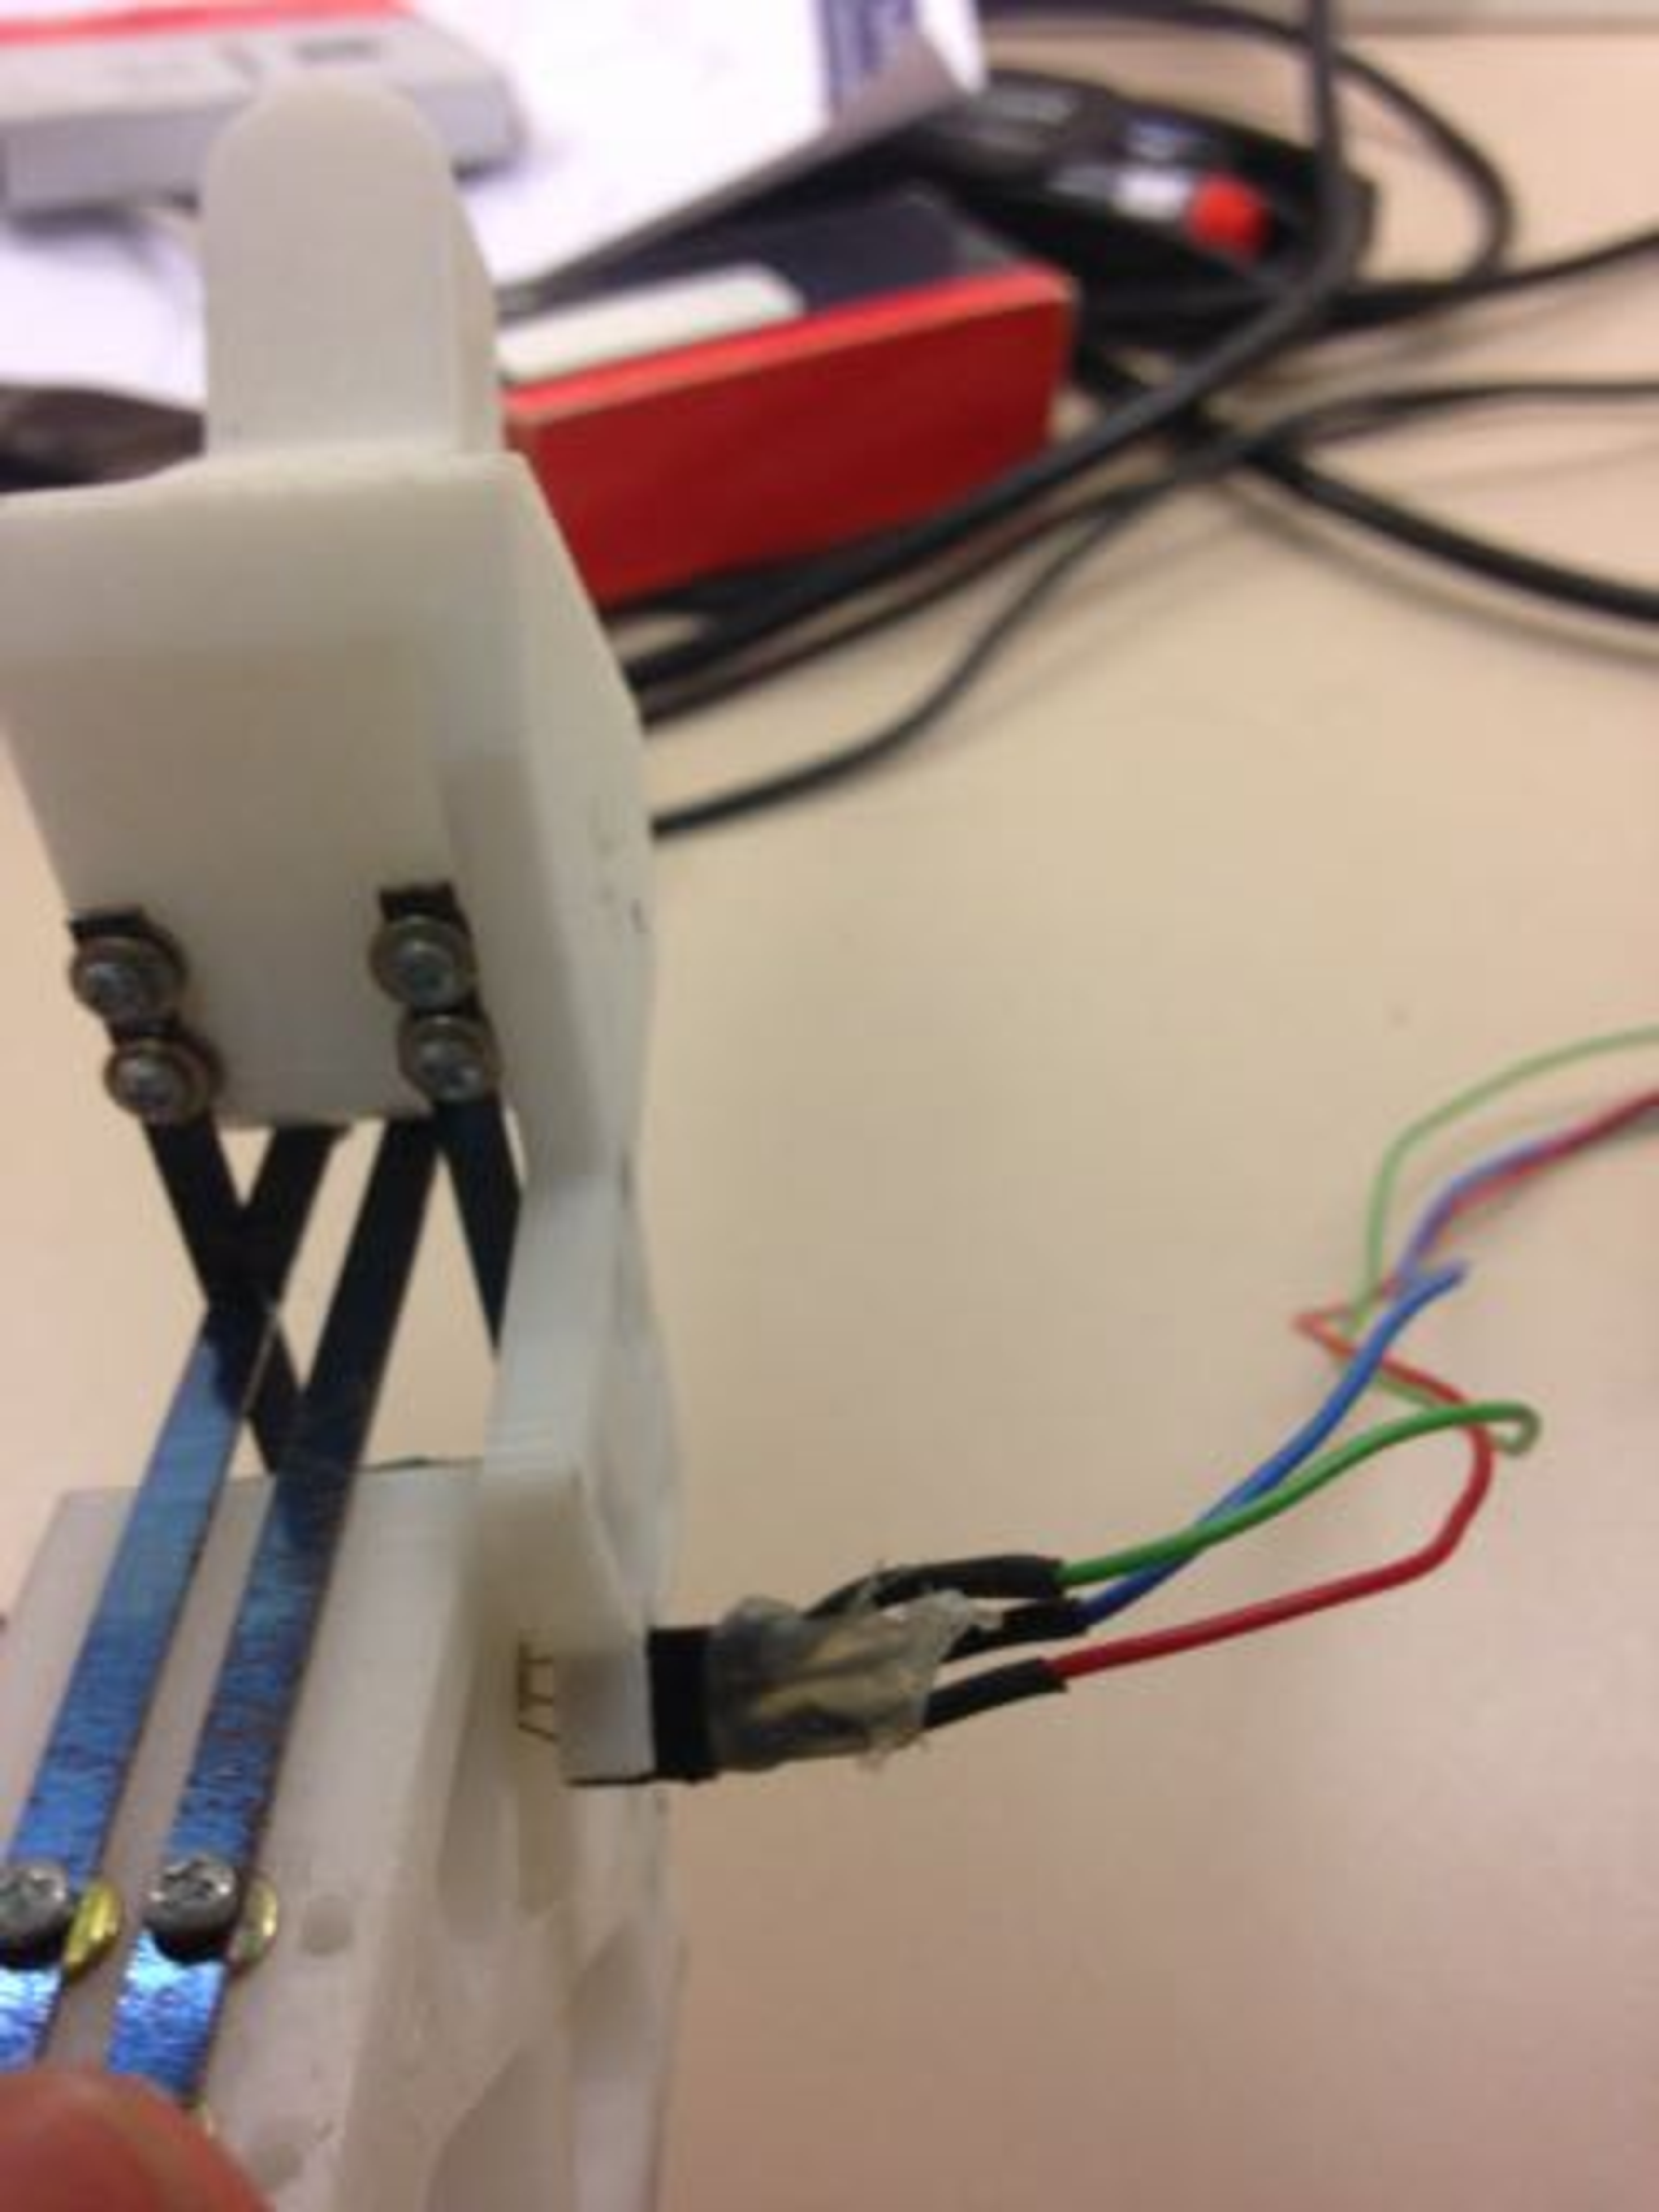
\includegraphics[width=3mm]{./figures/sensor_solder2.pdf}}
\item Screw in the metal strips on the handle part. Using a toothpick and positioning base is very handy for alligning the screws with nuts. 
\zoombox{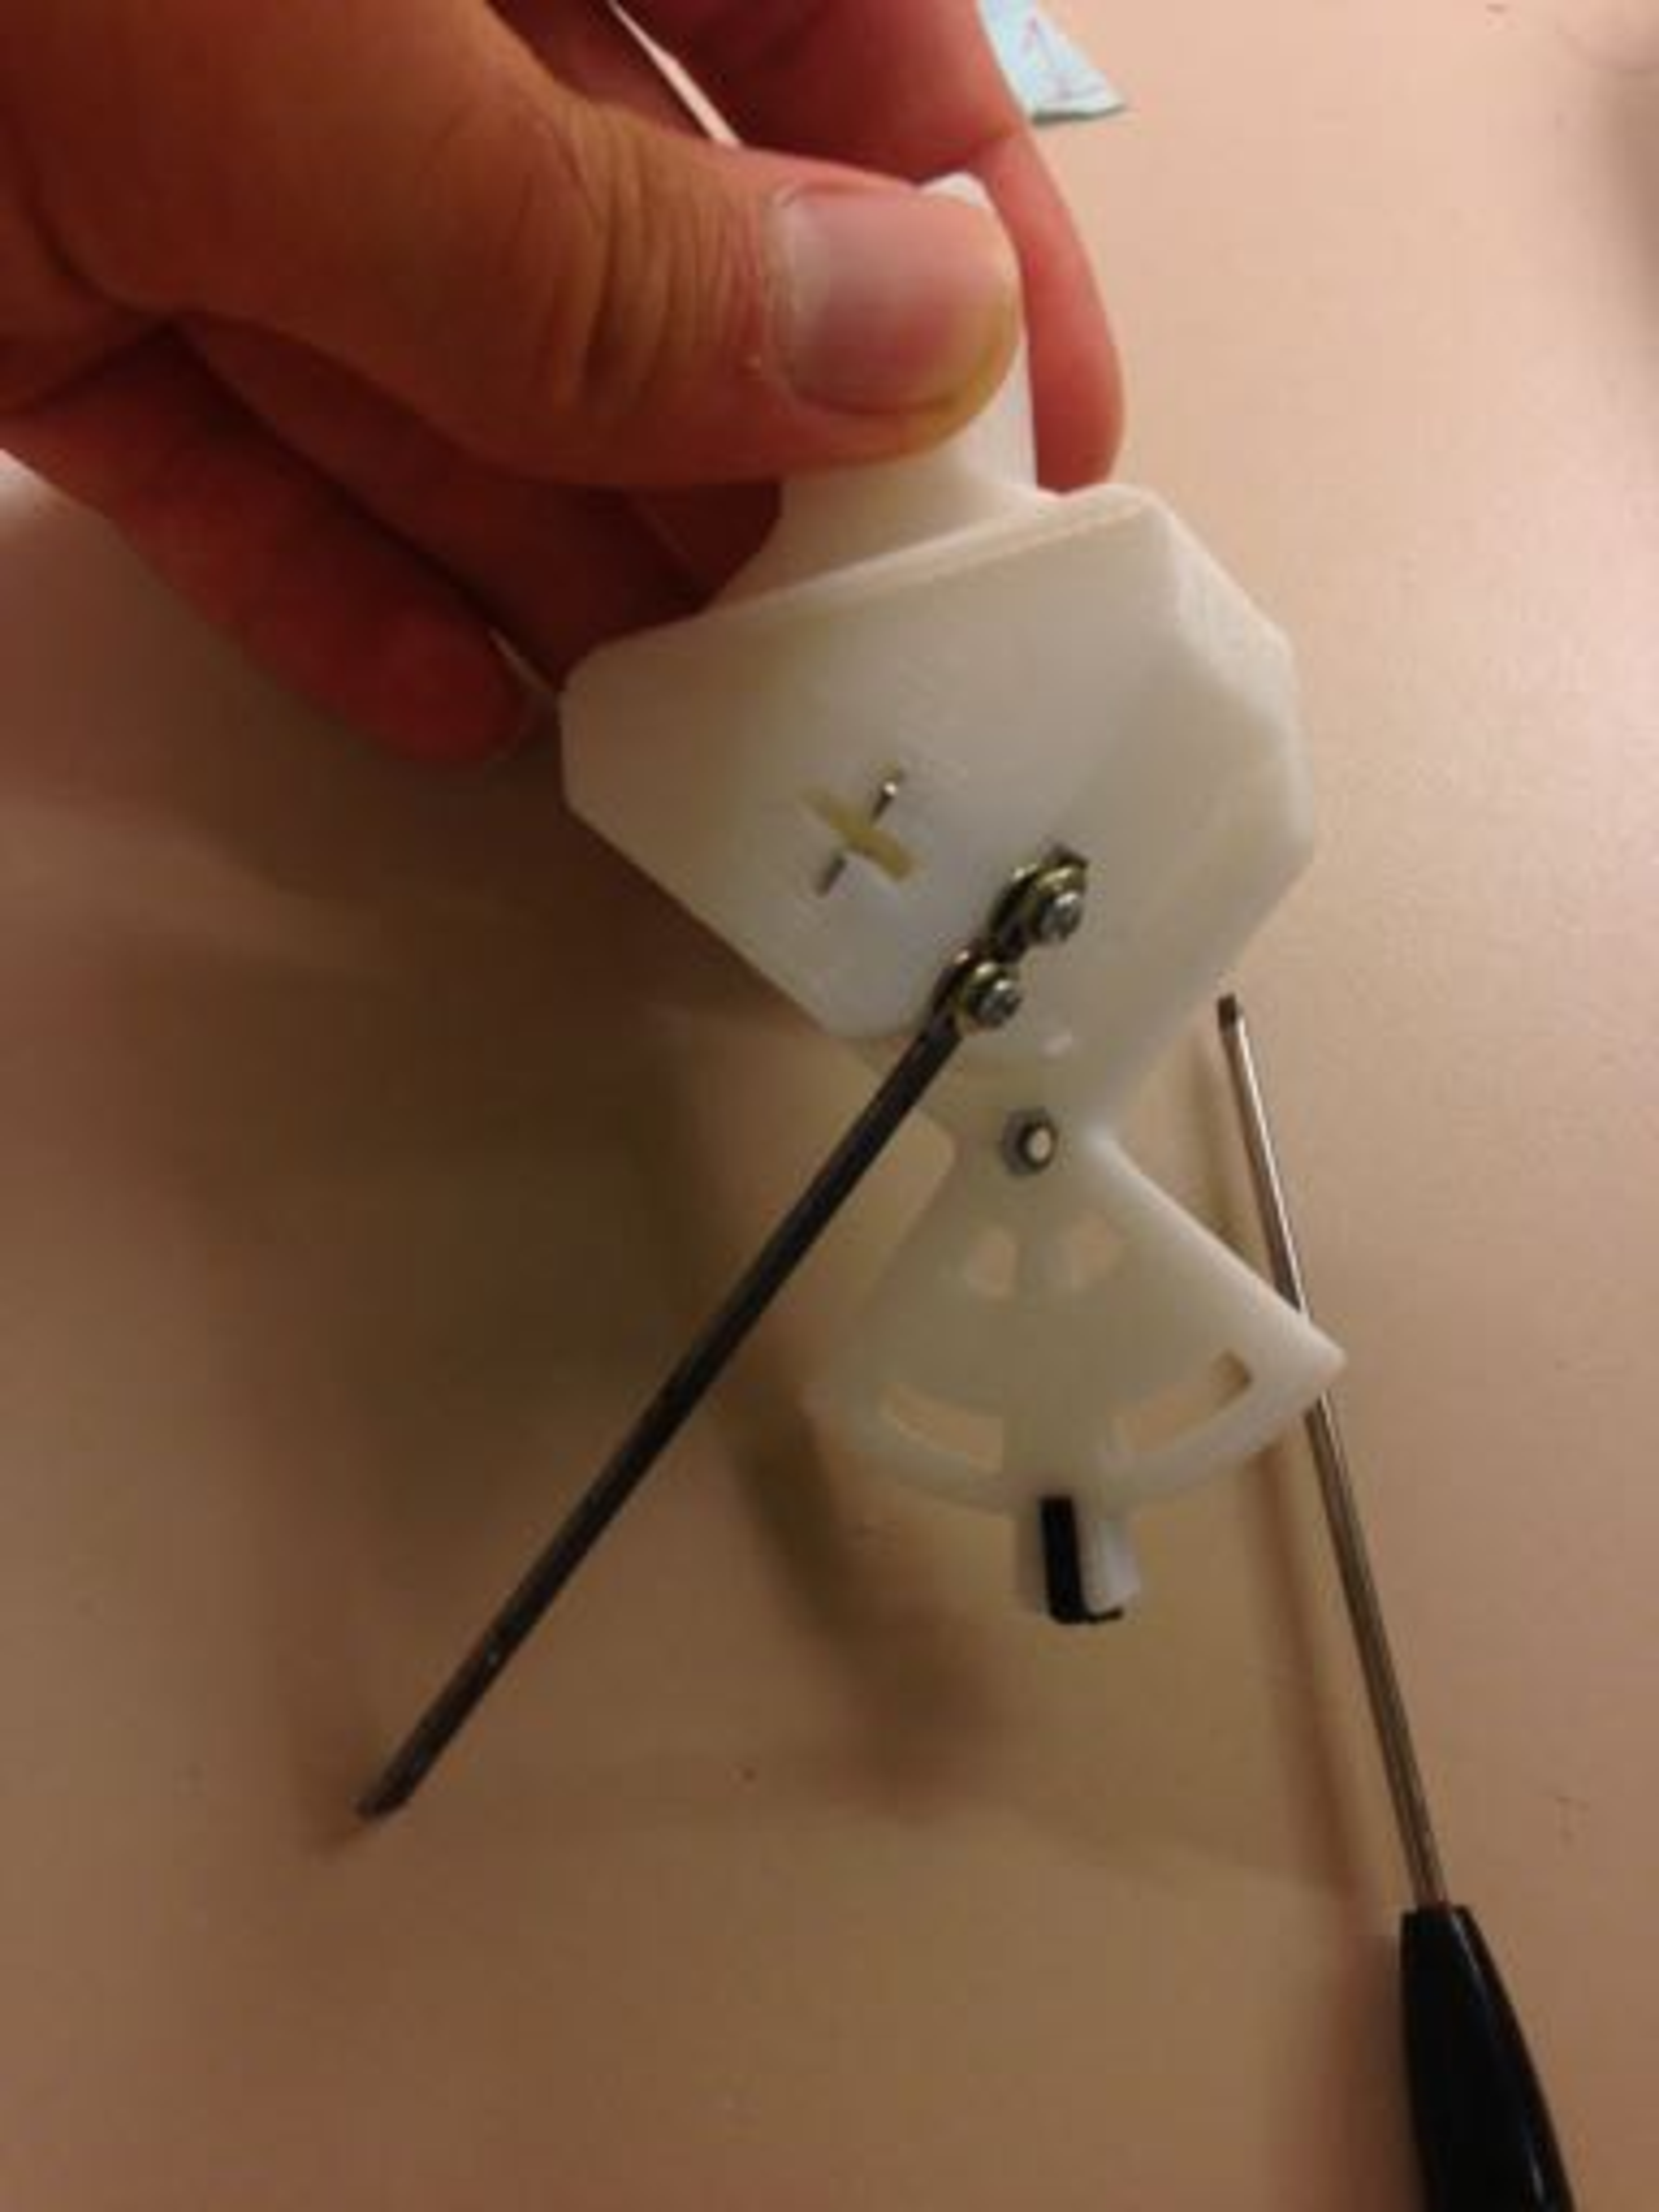
\includegraphics[width=3mm]{./figures/handle_1spring.pdf}}
\zoombox{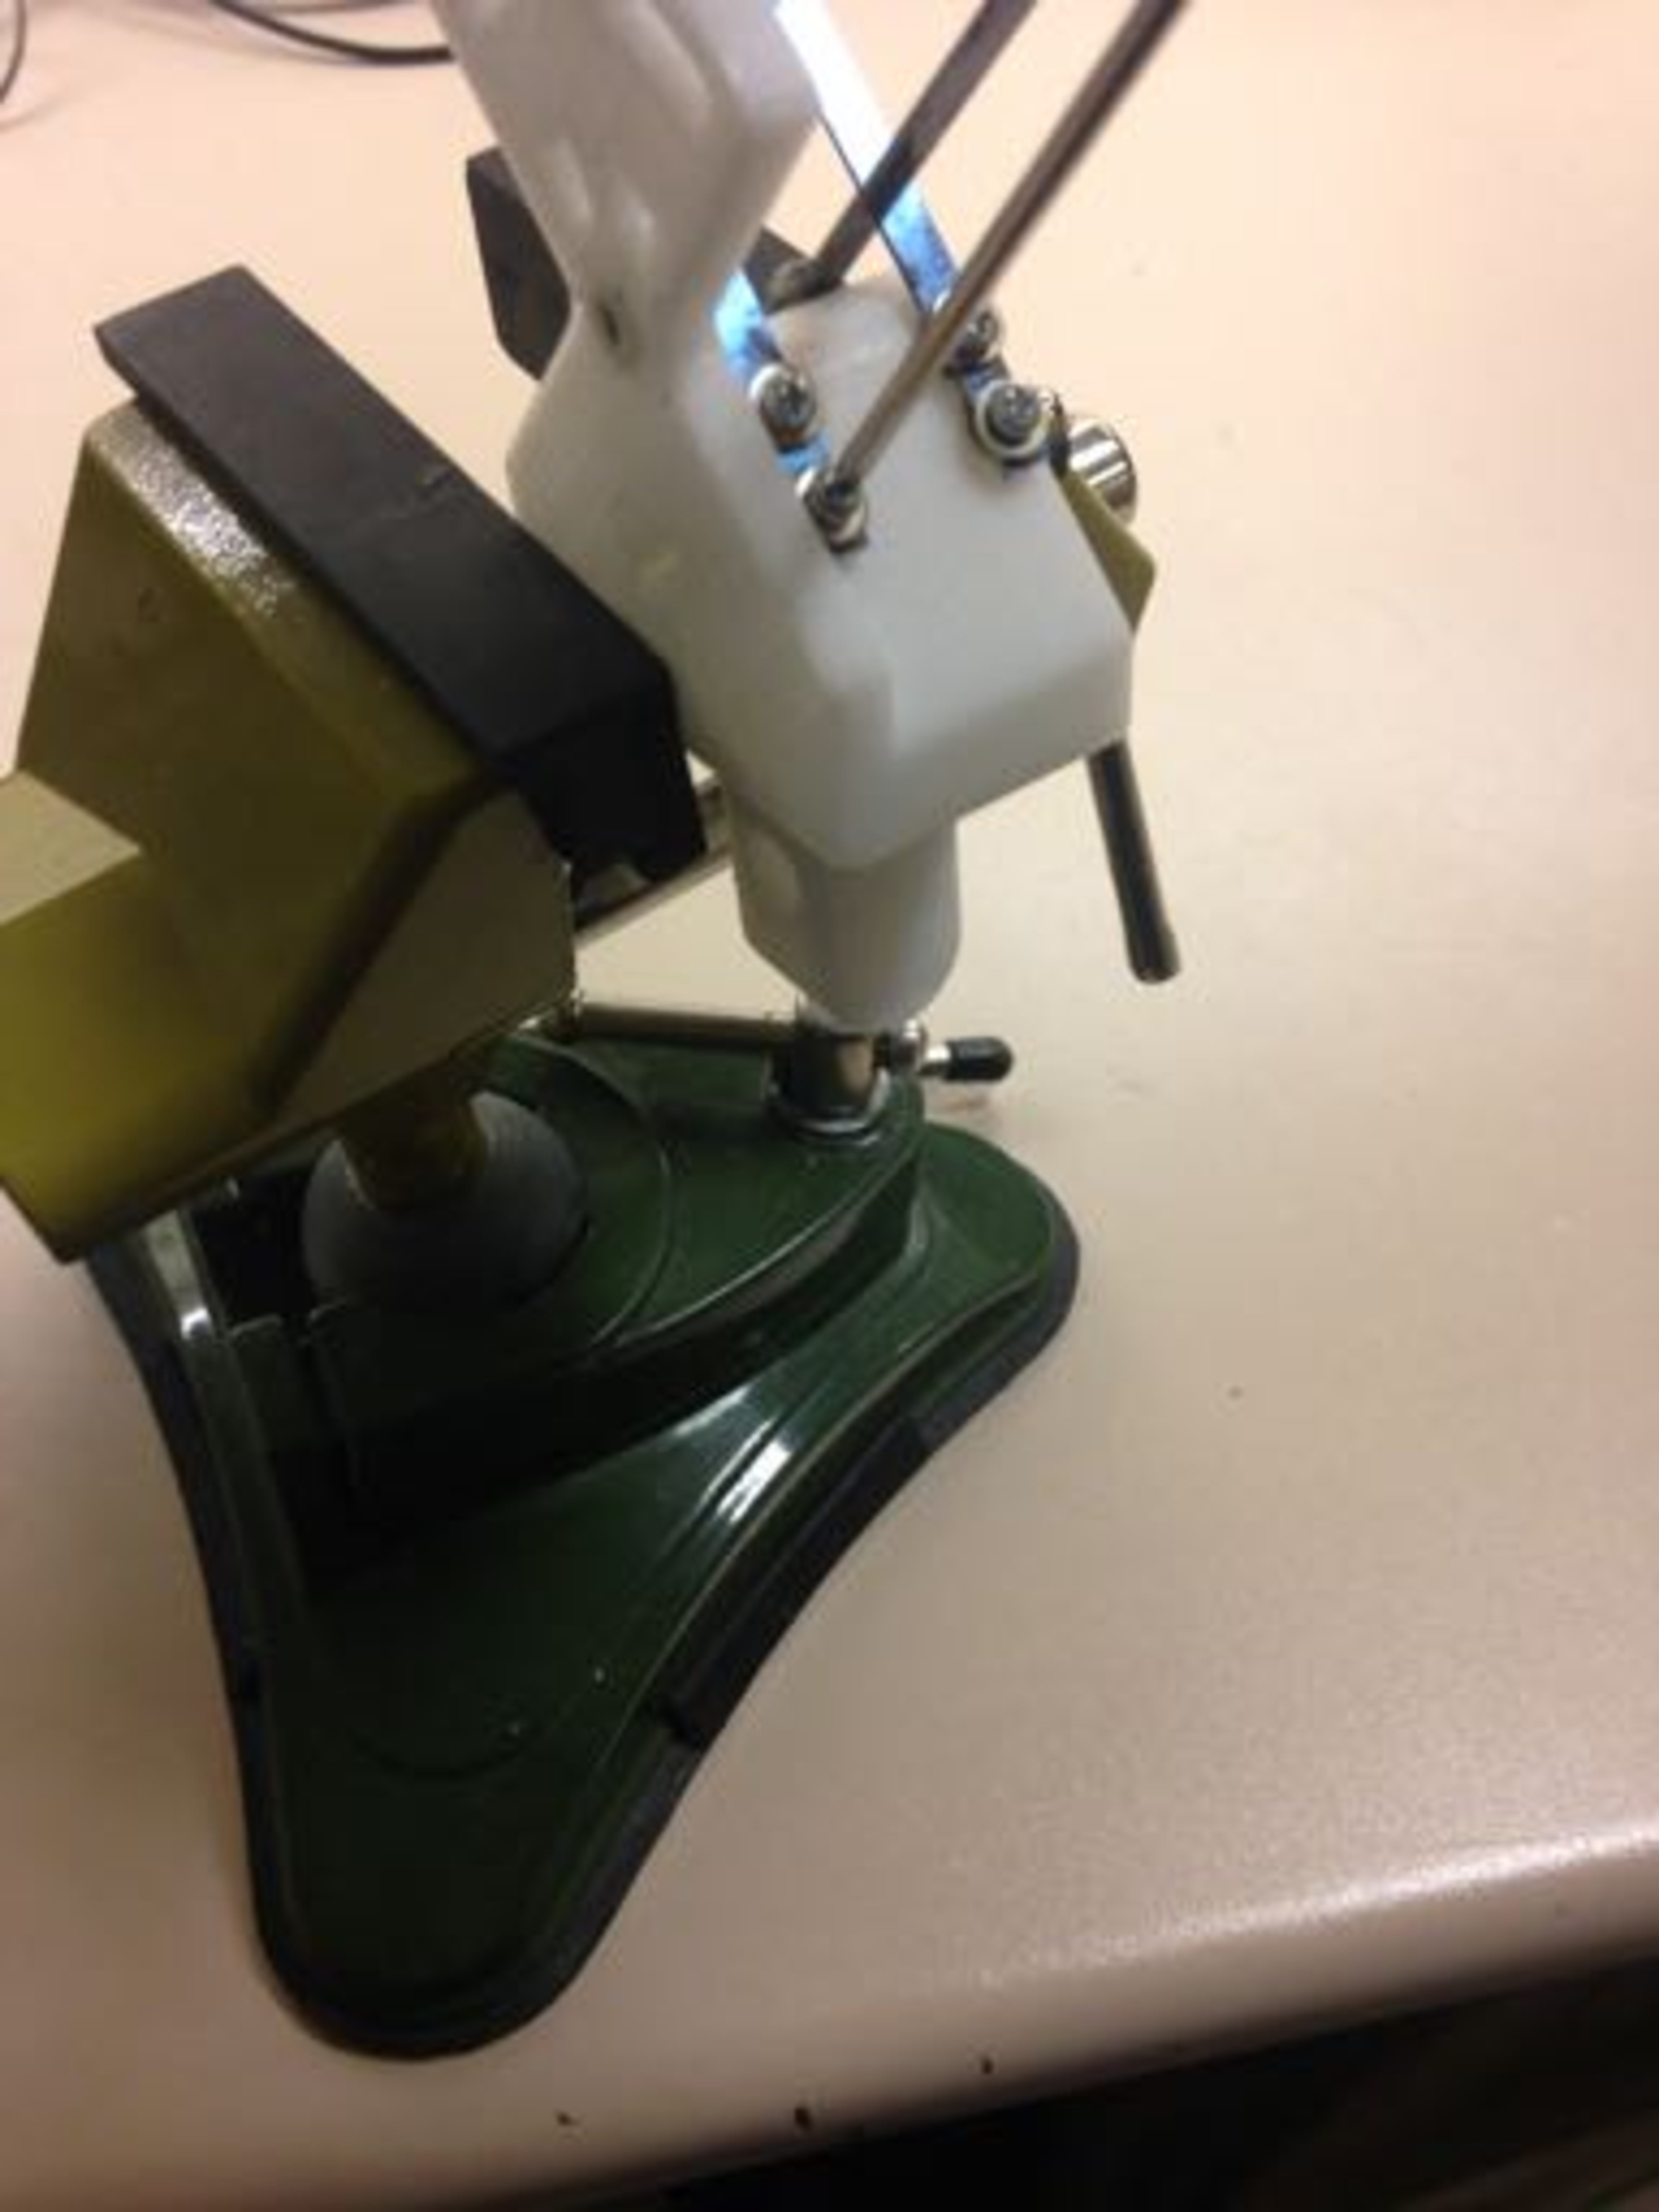
\includegraphics[width=3mm]{./figures/handle_screw.pdf}}
\item Screw in the metal strips on the pulley part.
\zoombox{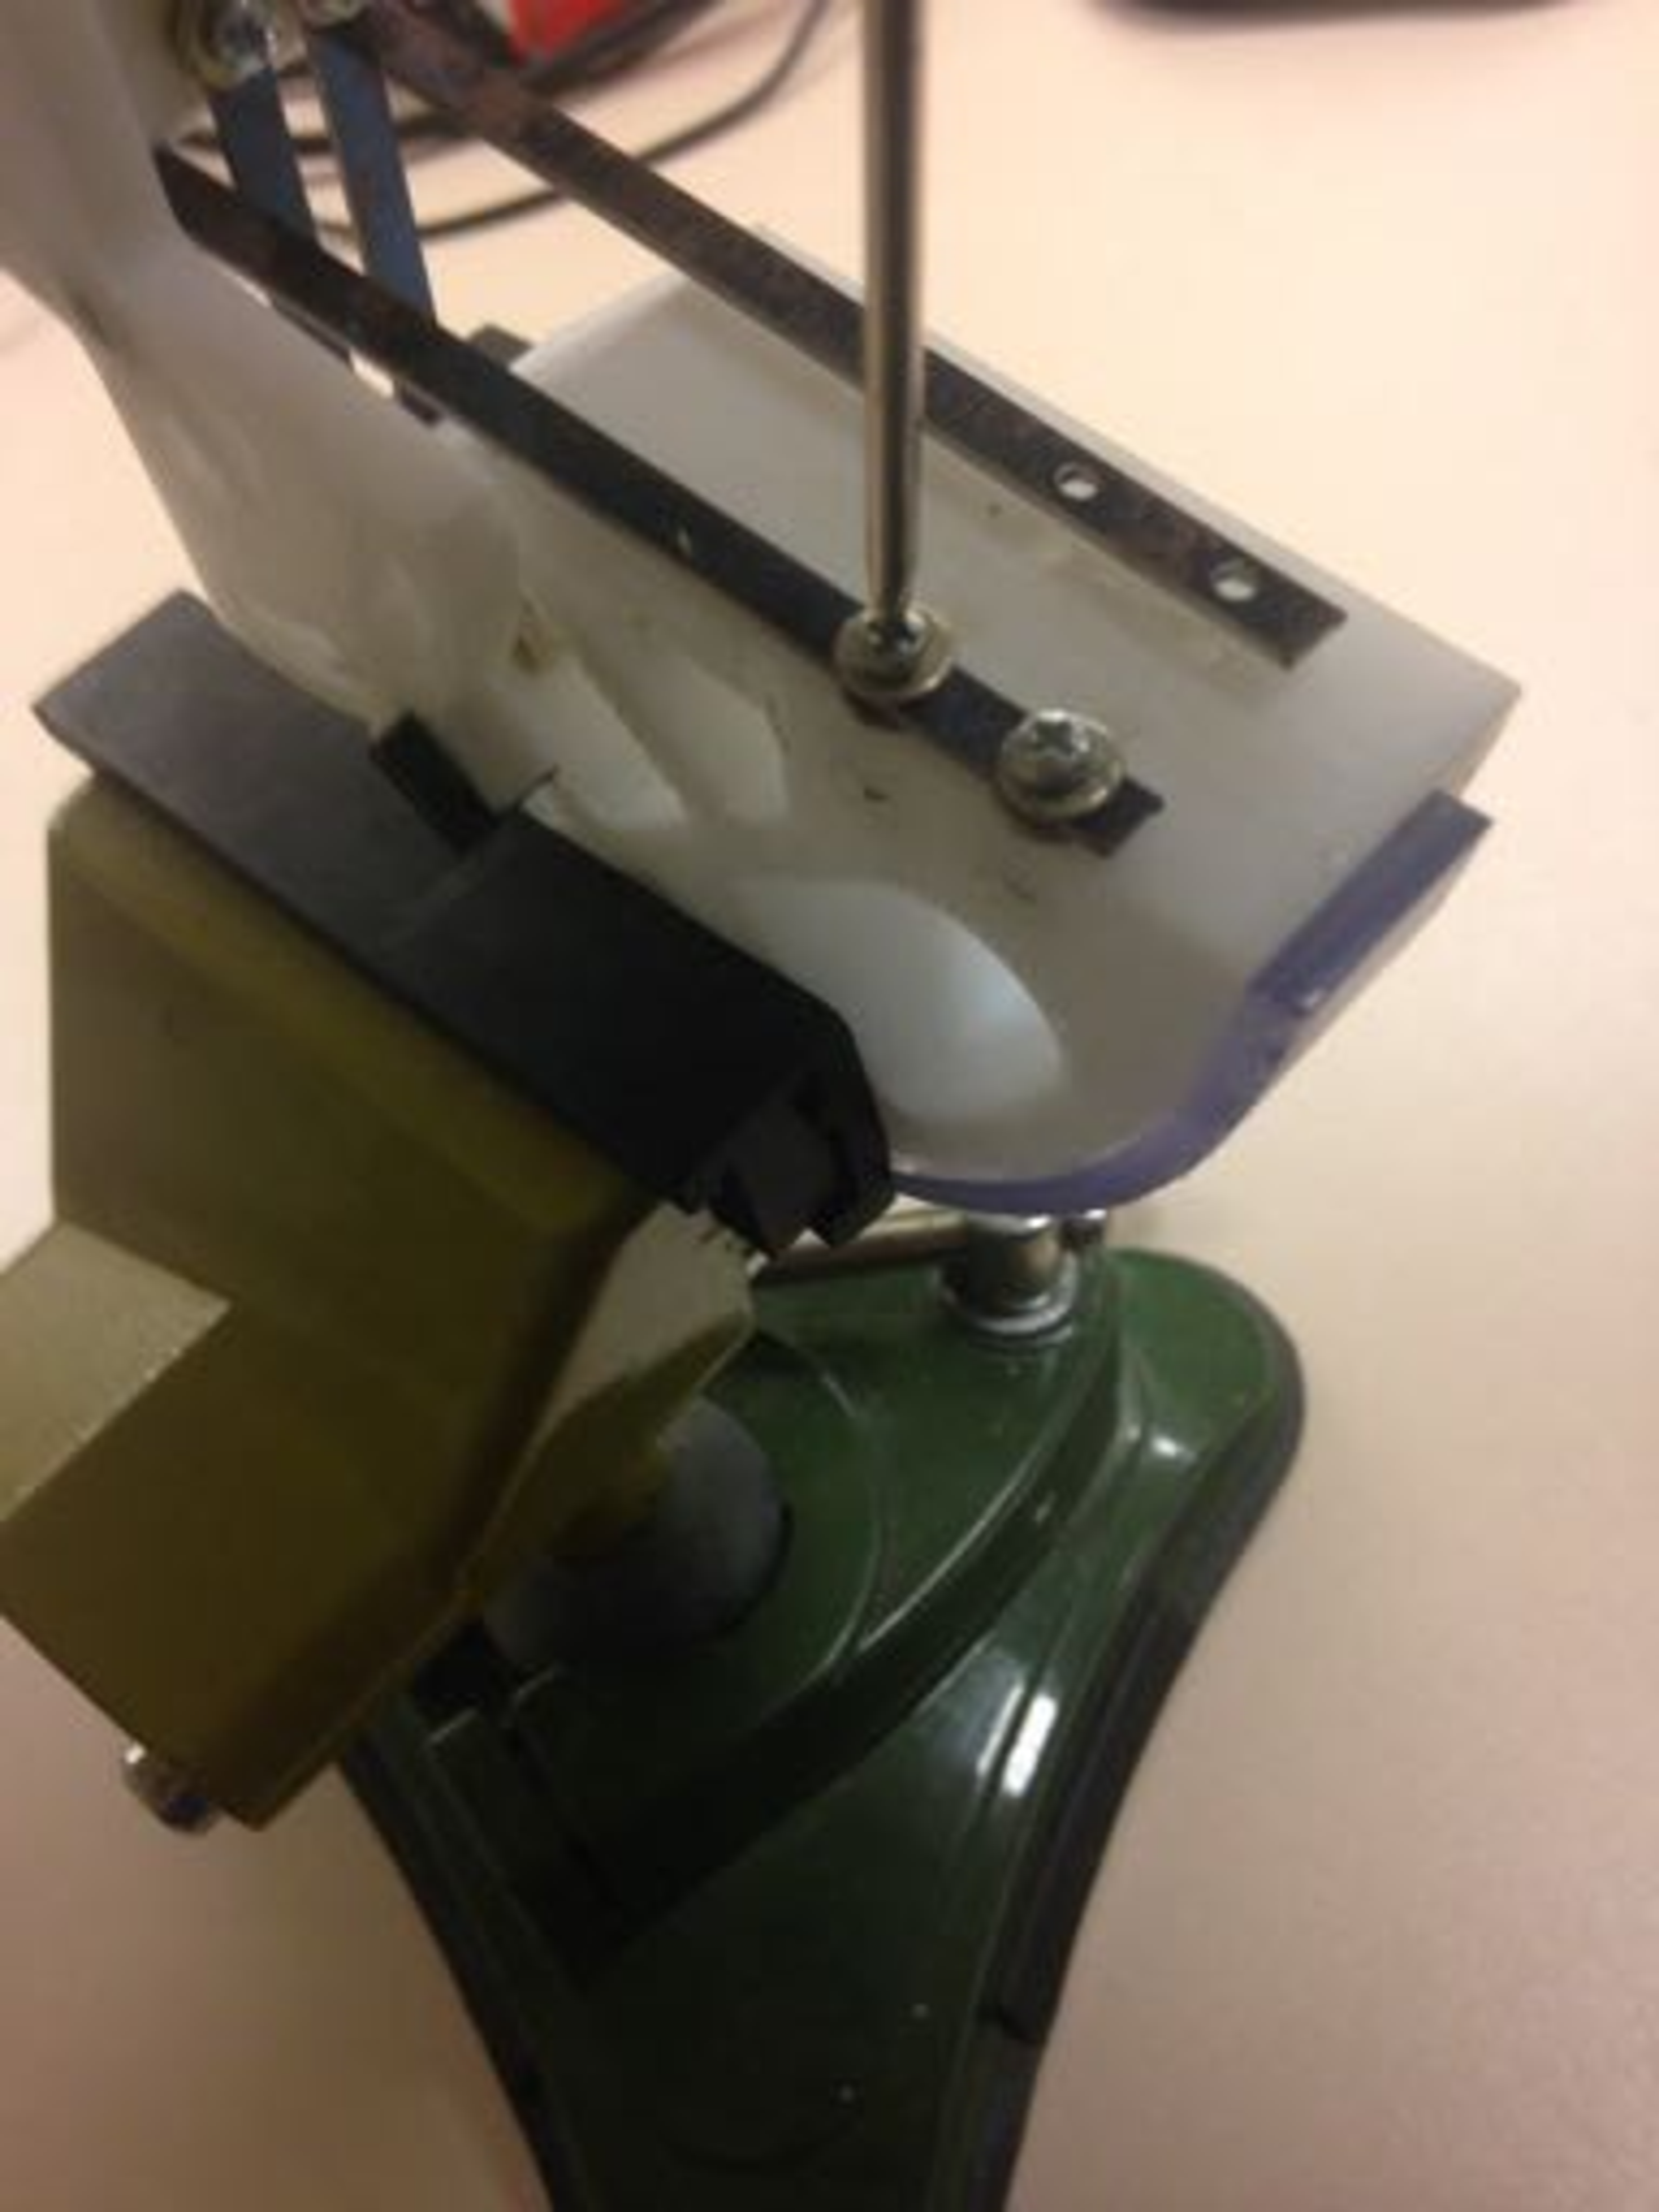
\includegraphics[width=3mm]{./figures/pulley_screw.pdf}}
\end{enumerate}
\end{itemize}
\scriptsize
The end product of this section should look like:
\zoombox{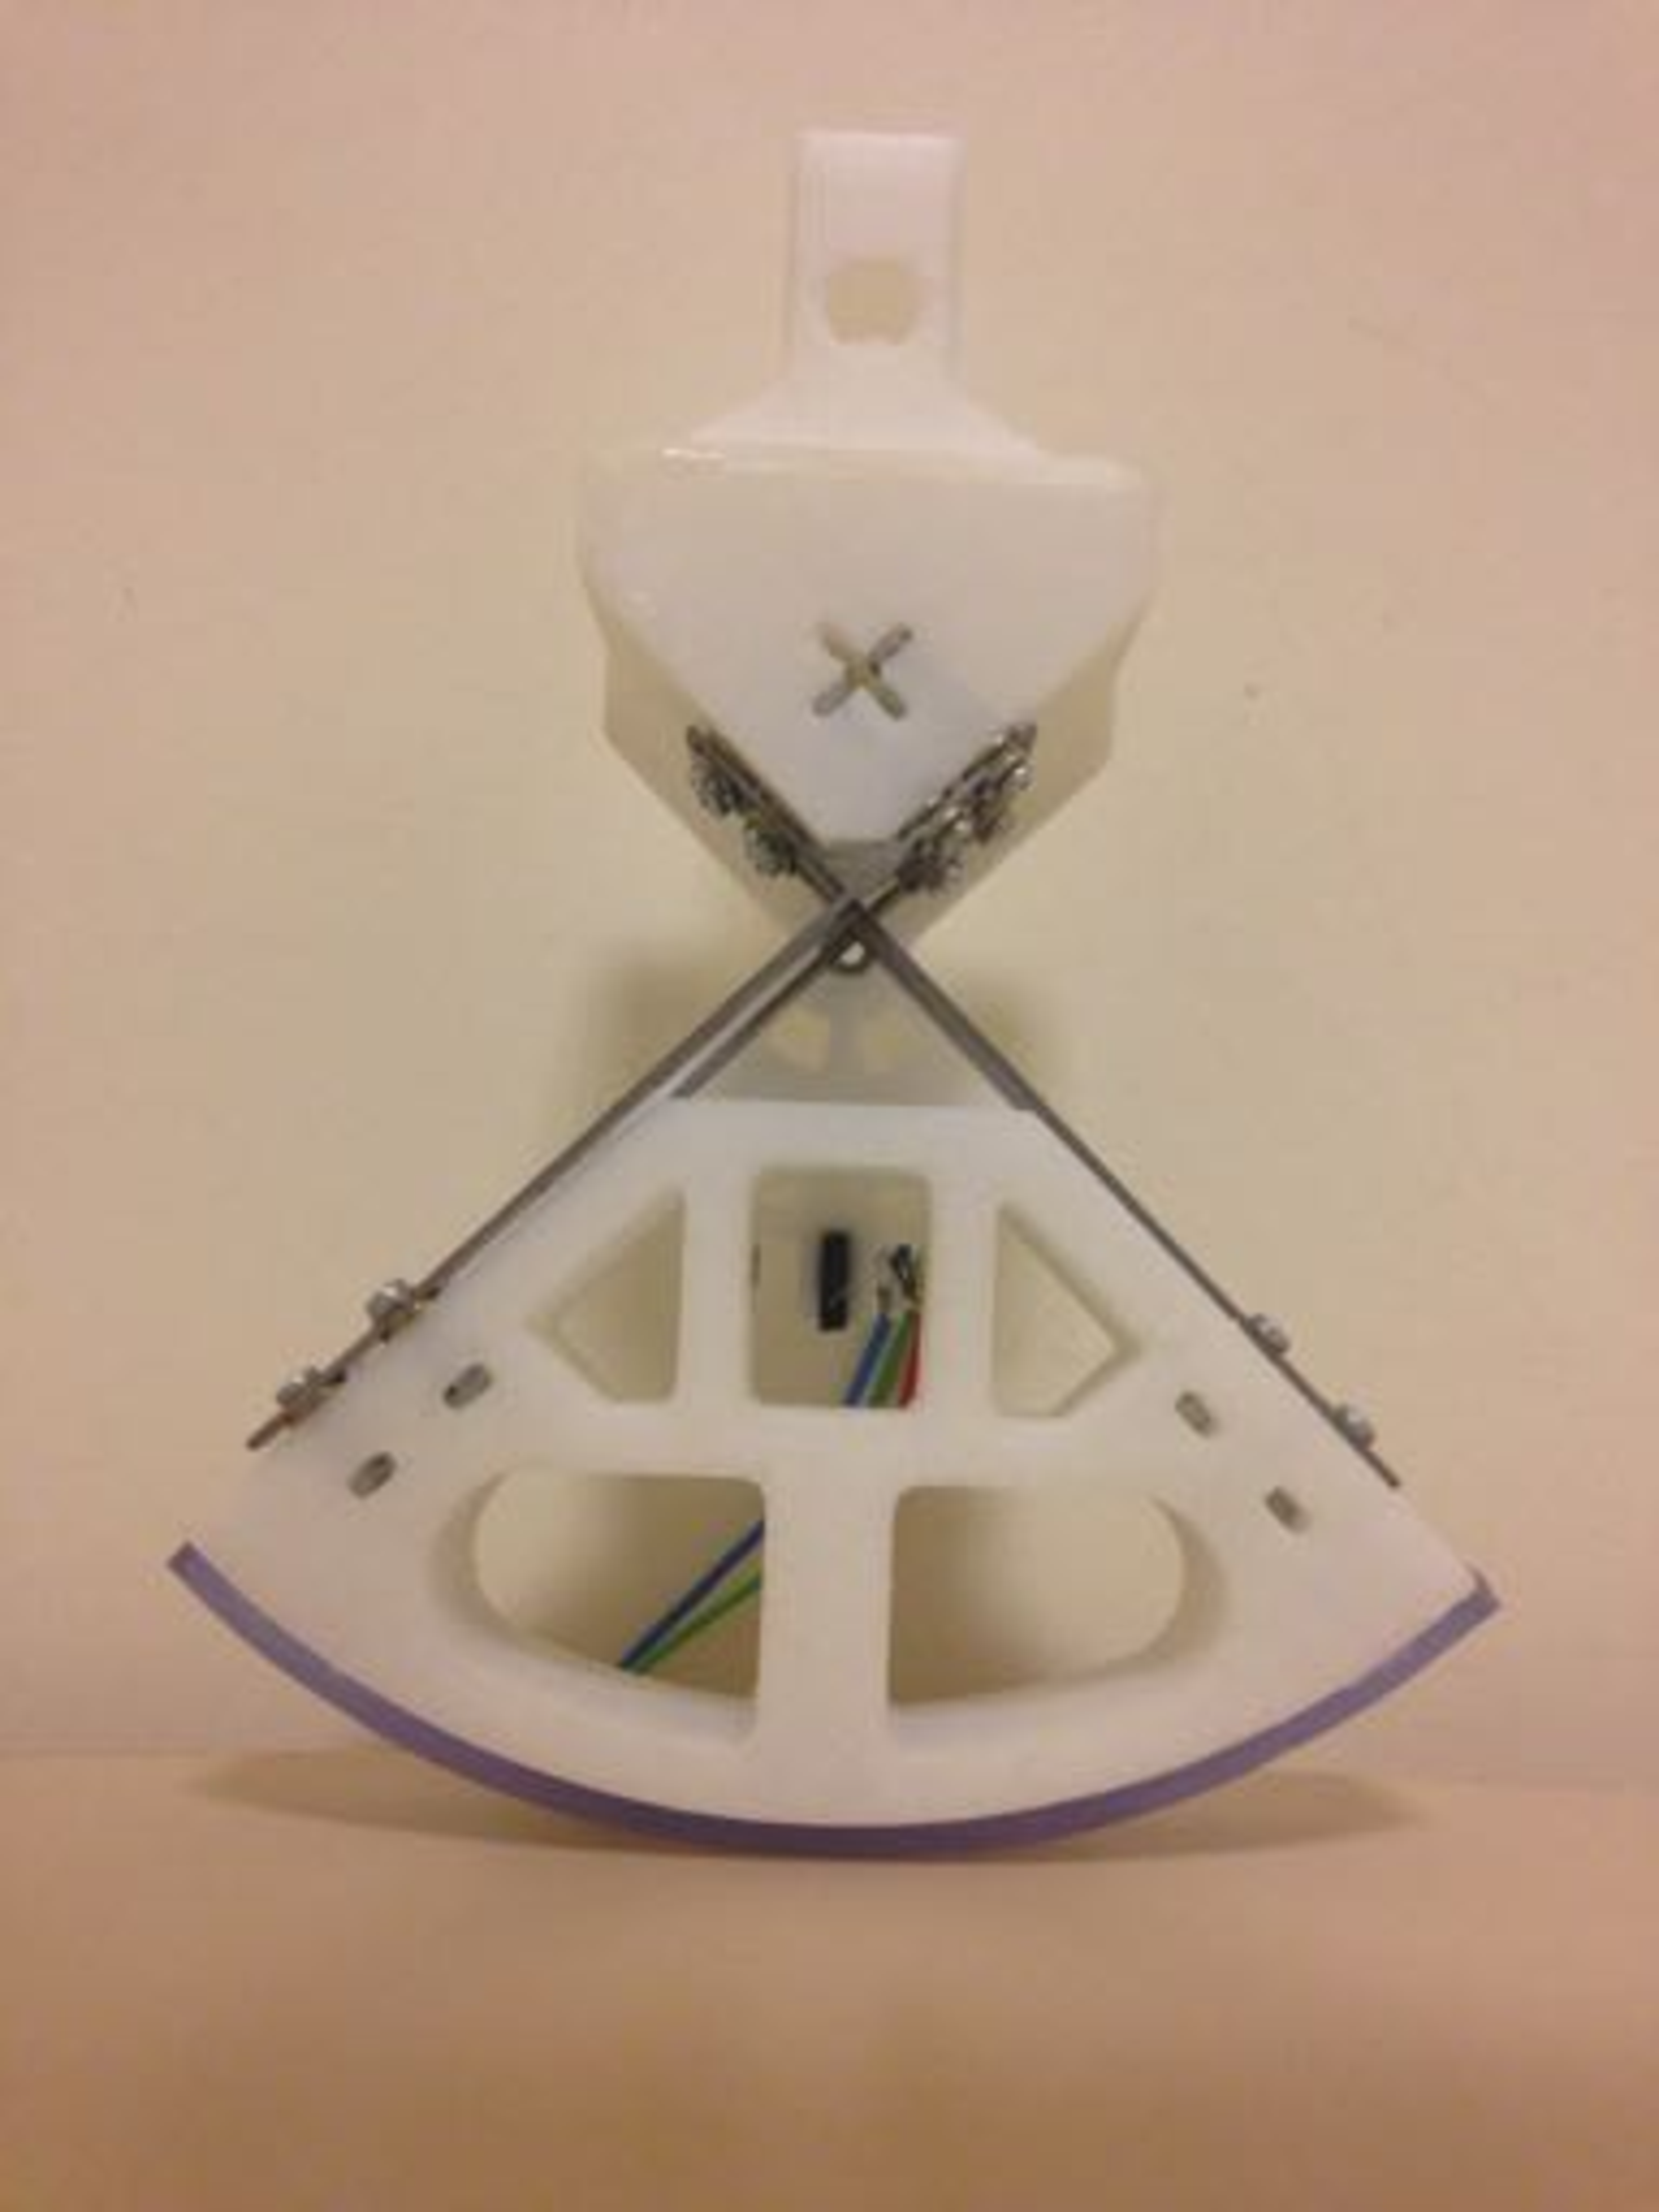
\includegraphics[width=3mm]{./figures/assembled_top.pdf}}
\newline
Note: This is the only time consuming part of the assembly. 
\end{frame}

\begin{frame}[t]{Mounting the motor and top}
\begin{itemize} 
\vspace{-4mm}
\item Components
\newline
\begin{minipage}{0.4\textwidth}
\begin{itemize} \scriptsize
\setlength\itemsep{-0.3mm}
\item Motor
\item Pinion
\item Motor holder
\item Shoulder screw
\item 3 mm thick PVC table cover
\end{itemize}
\end{minipage}
\begin{minipage}{0.5\textwidth}
\begin{itemize} \scriptsize
\setlength\itemsep{-0.5mm}
\item 3mm washer
\item 2x D:2 L:5 mm screws 
\item Heat shrink tube (wider than pinion)
\item Hot air gun
\end{itemize}
\end{minipage}
\item Procedure
\begin{enumerate} \scriptsize
\item Cut a piece of PVC table protector and paste it along the circumference of the pulley part as it is shown in the figure. The width of the PVC strip that we use is 15 mm but this can vary. The thickness can also vary. 
\item Use the shoulder screw and a washer to screw the handle part to the face through the bearing.
\zoombox{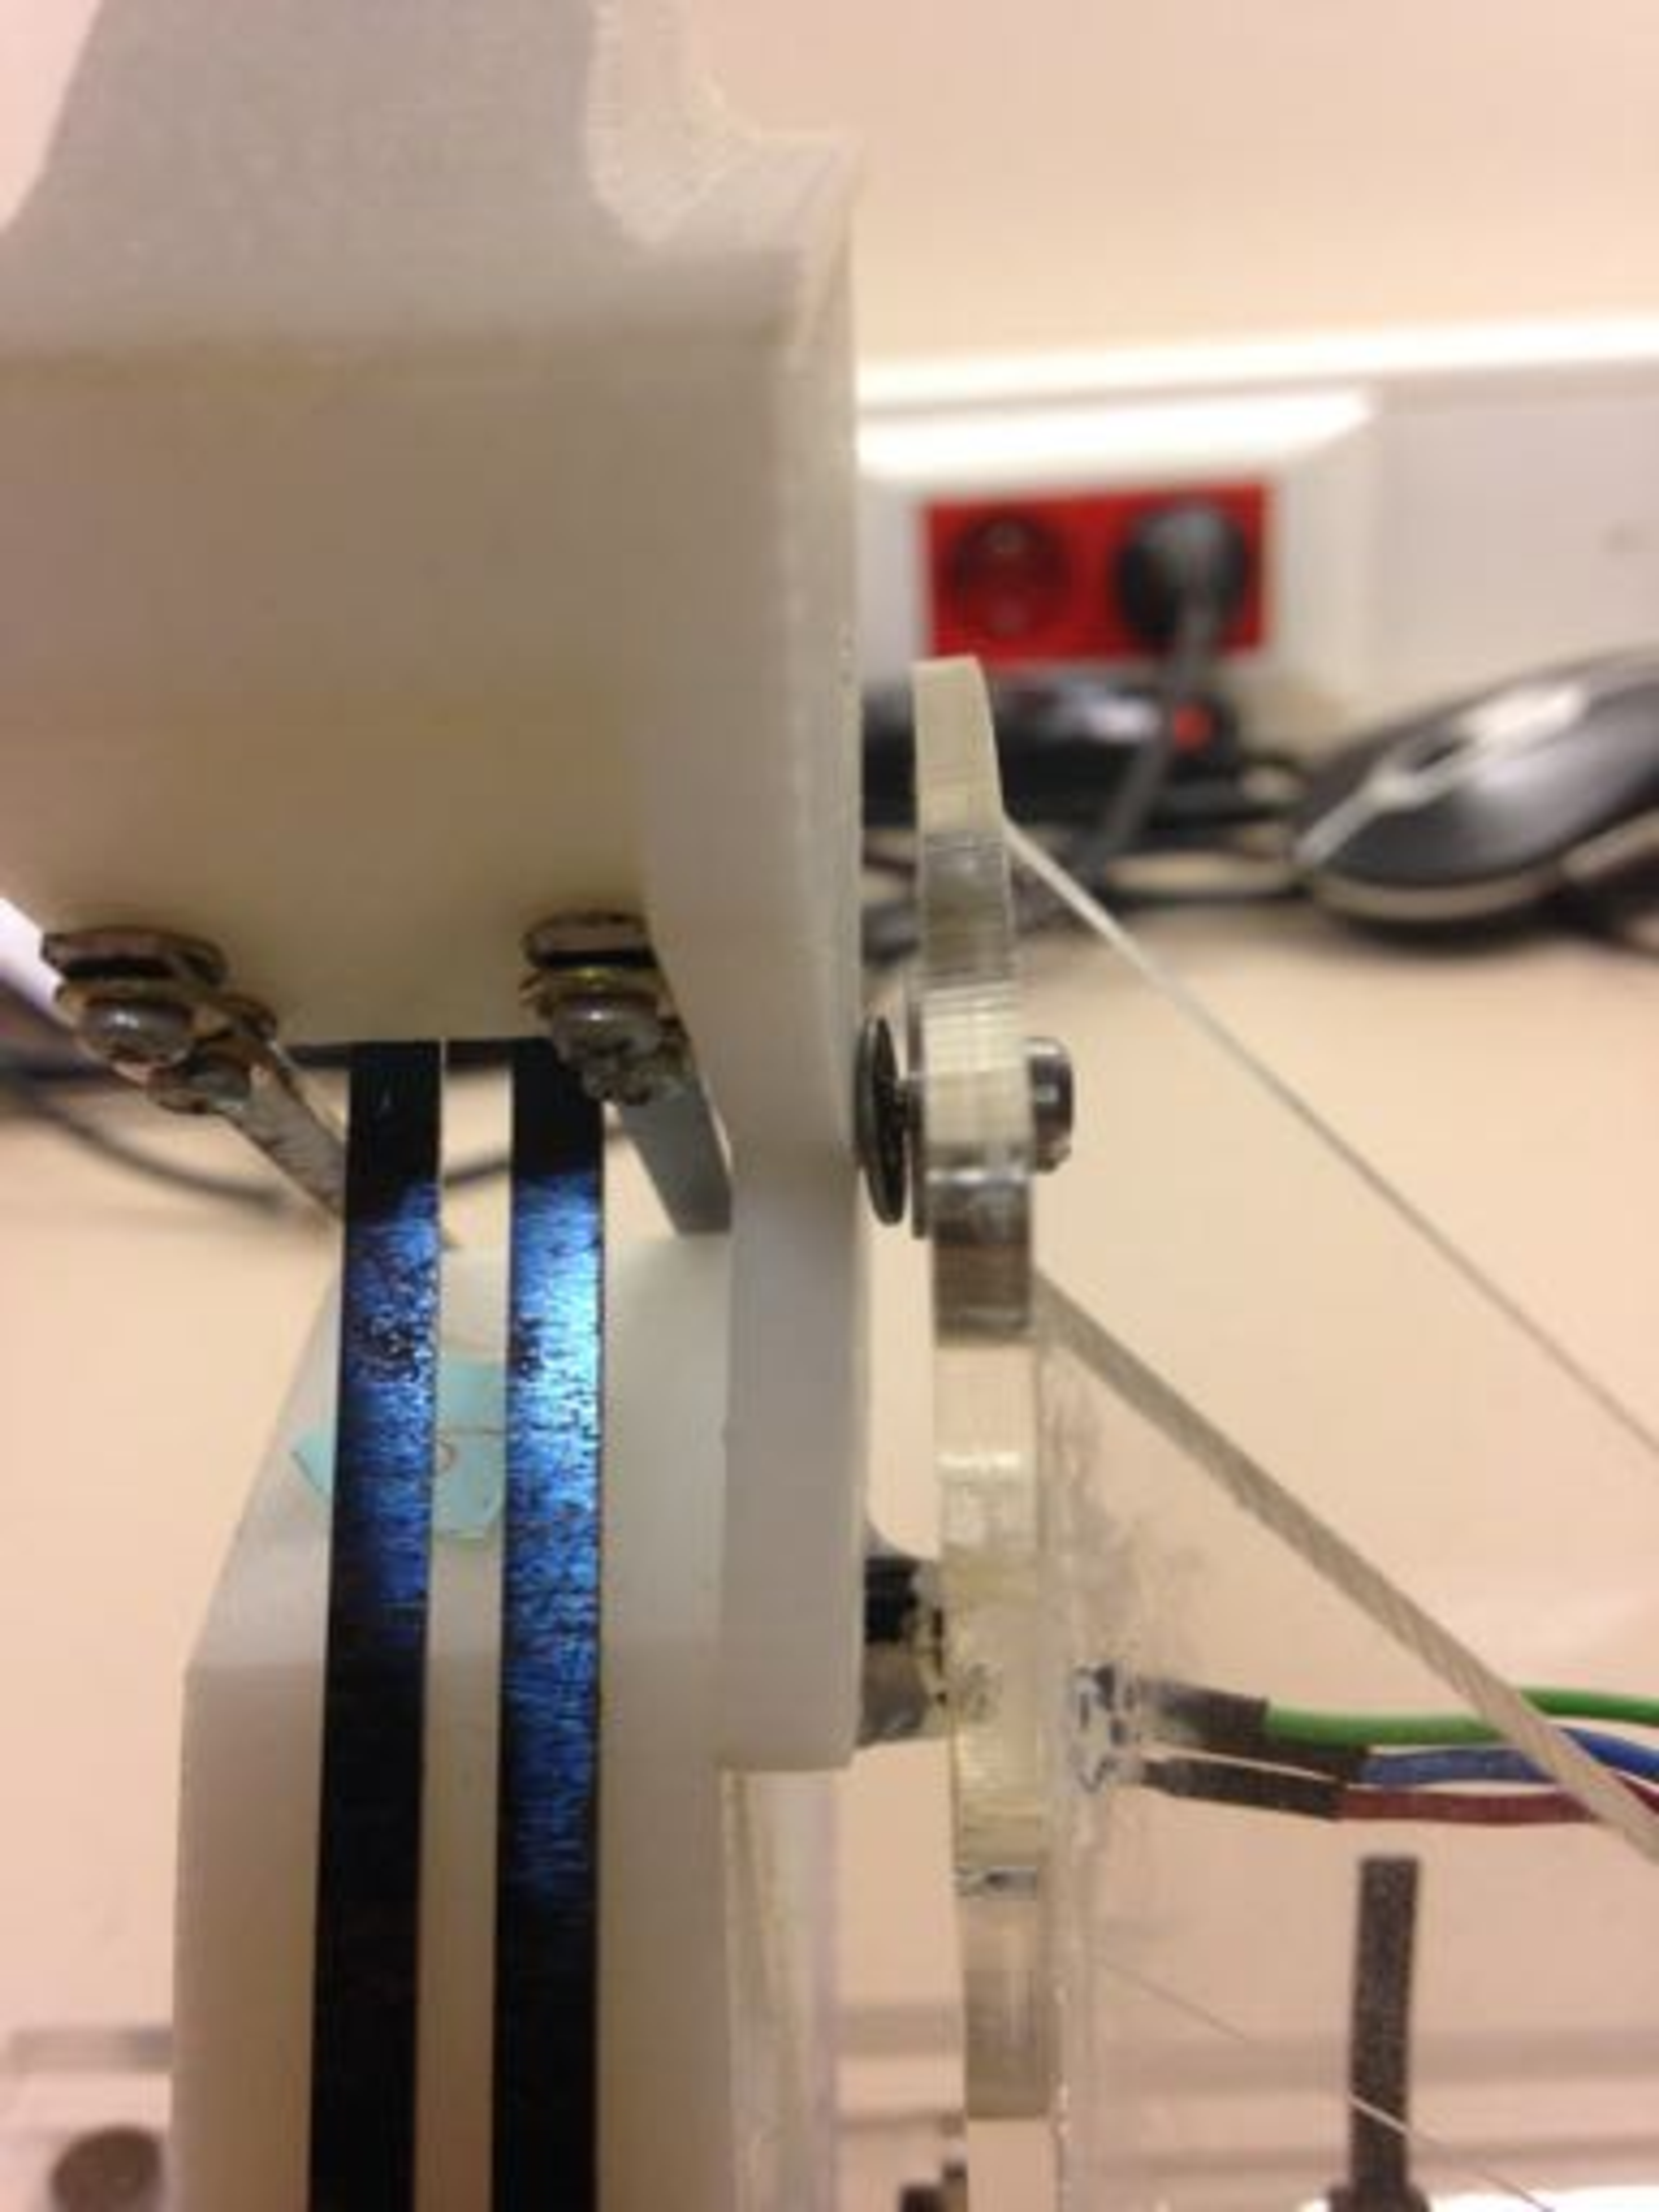
\includegraphics[width=3mm]{./figures/shoulder_screw.pdf}}
\zoombox{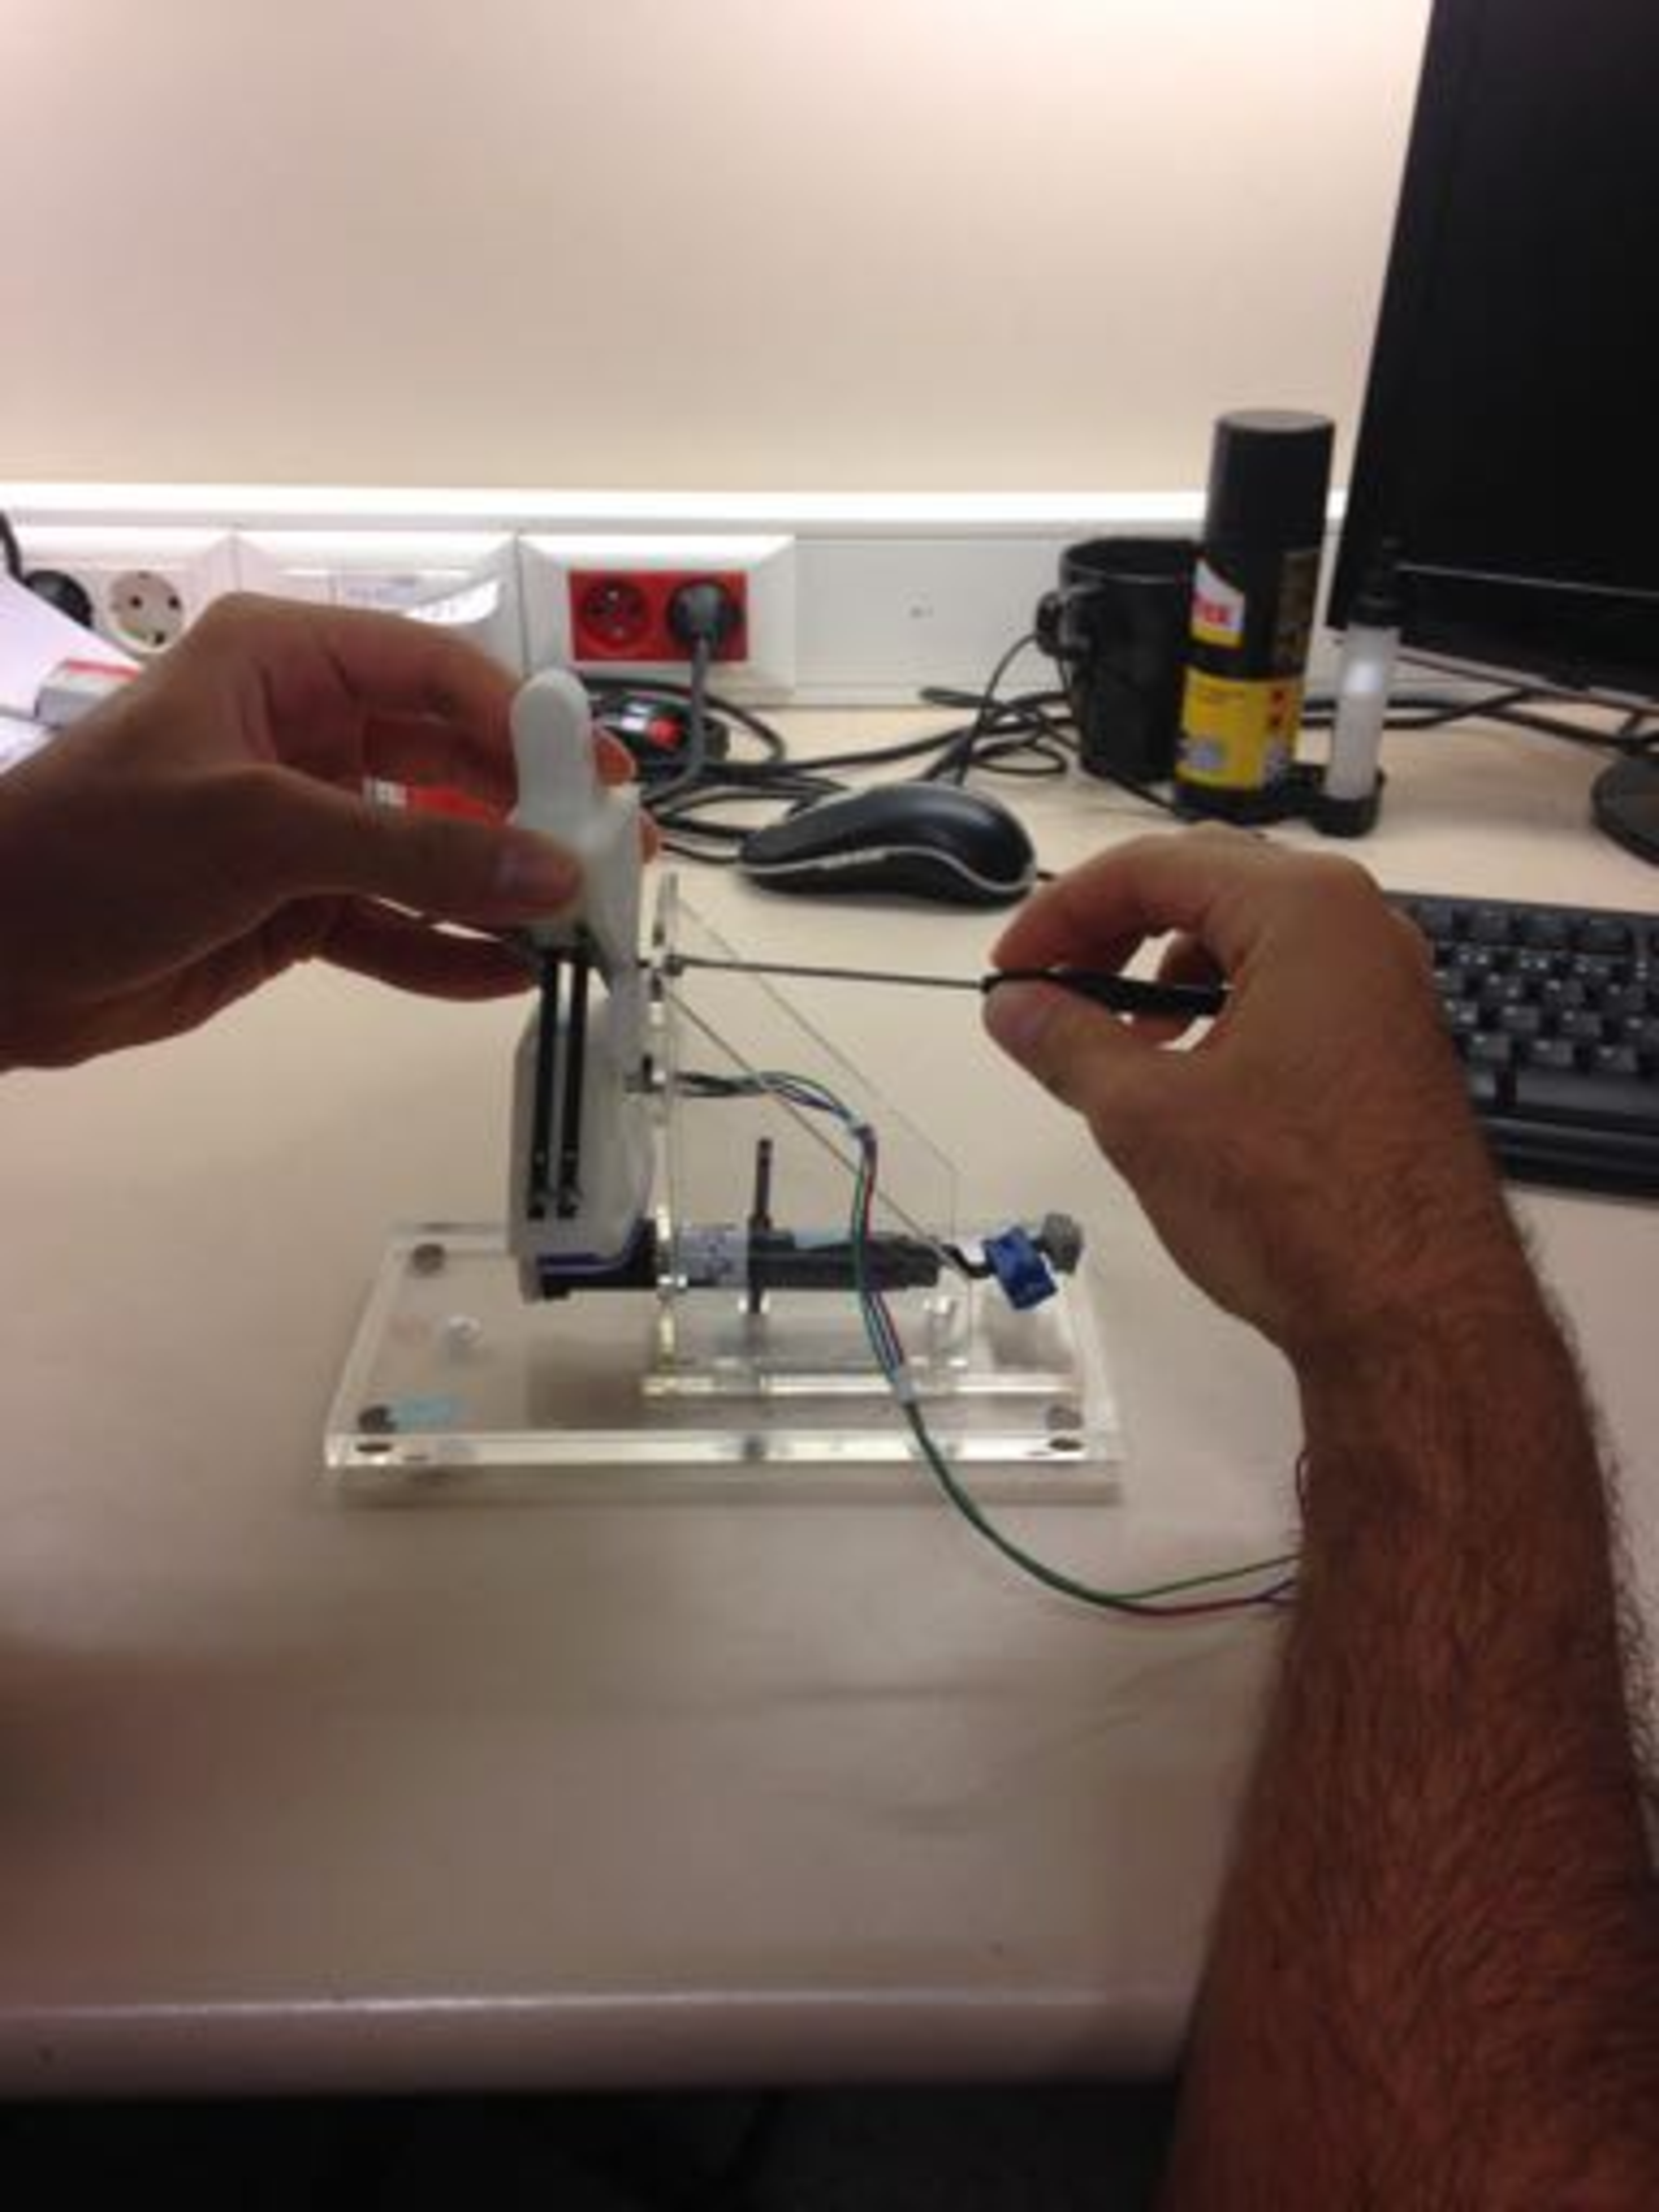
\includegraphics[width=3mm]{./figures/shoulder_screw2.pdf}}
\item Screw the motor holder on the motor.
\zoombox{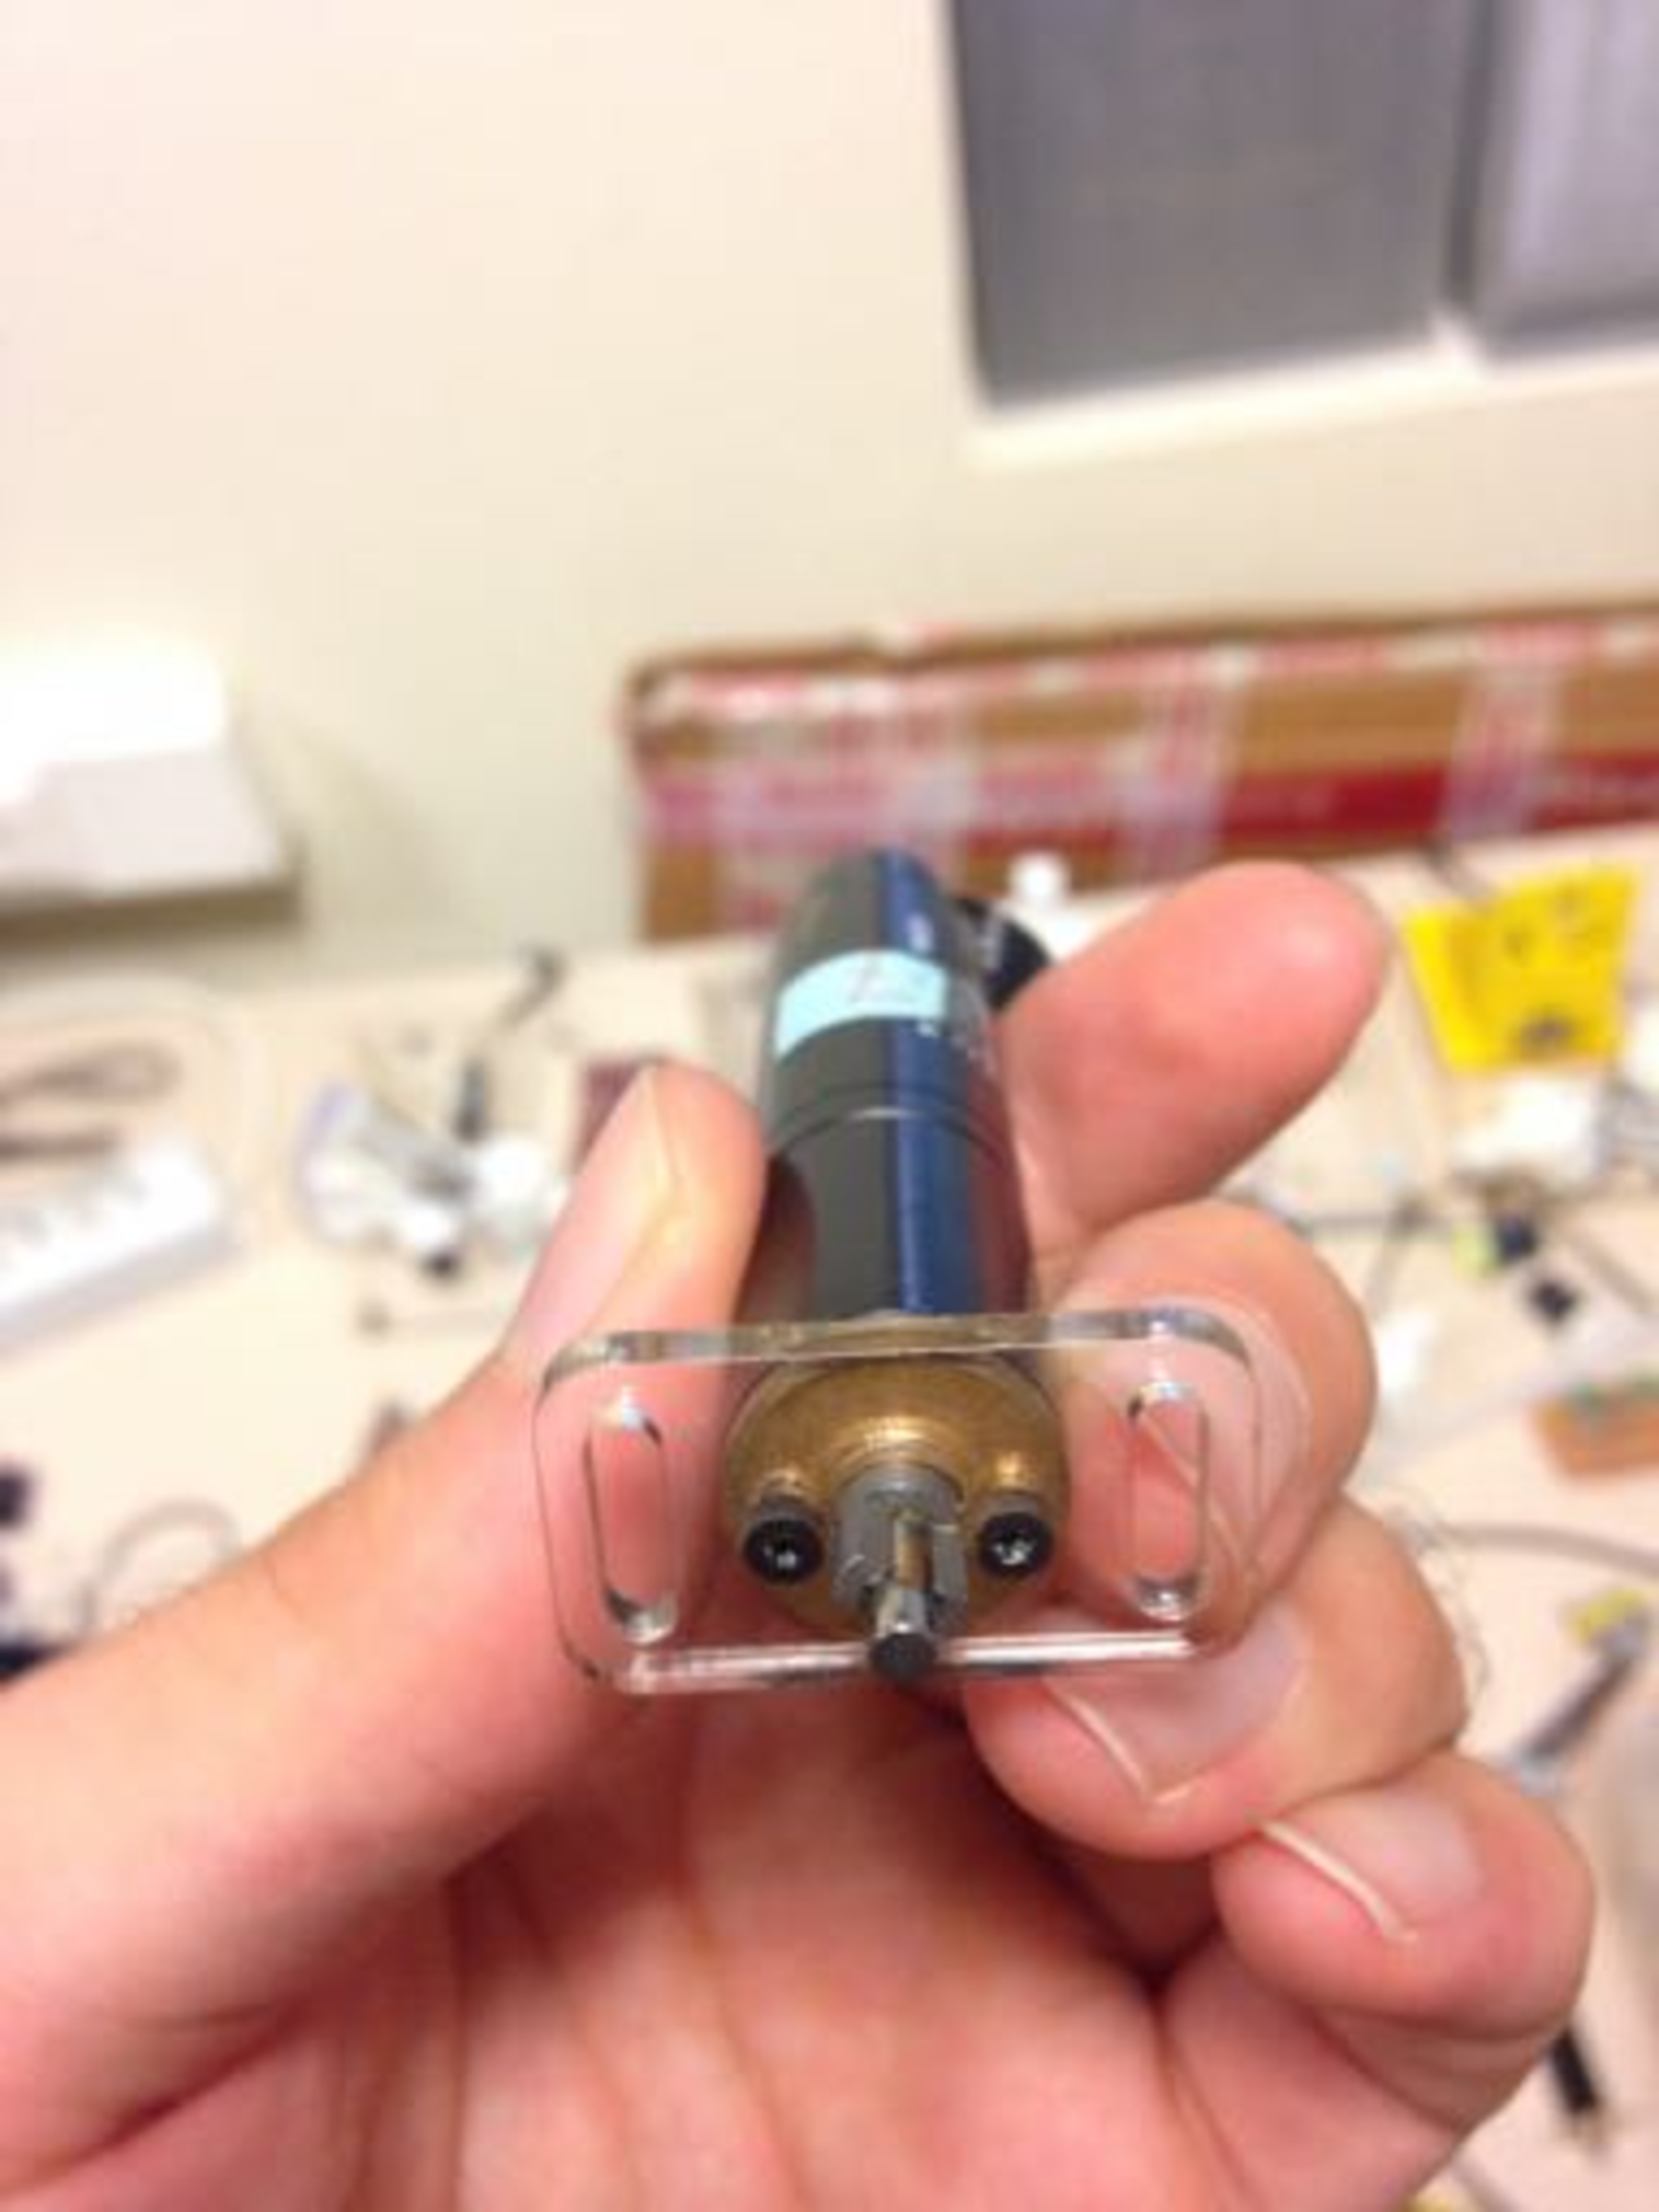
\includegraphics[width=3mm]{./figures/motor_front.pdf}}
\item Using a hot air gun wind a heat shrink tube around the pinion to avoid slip. Pinion's tip has a greater radius for restraining the pulley from tilting forwards during operation.
\zoombox{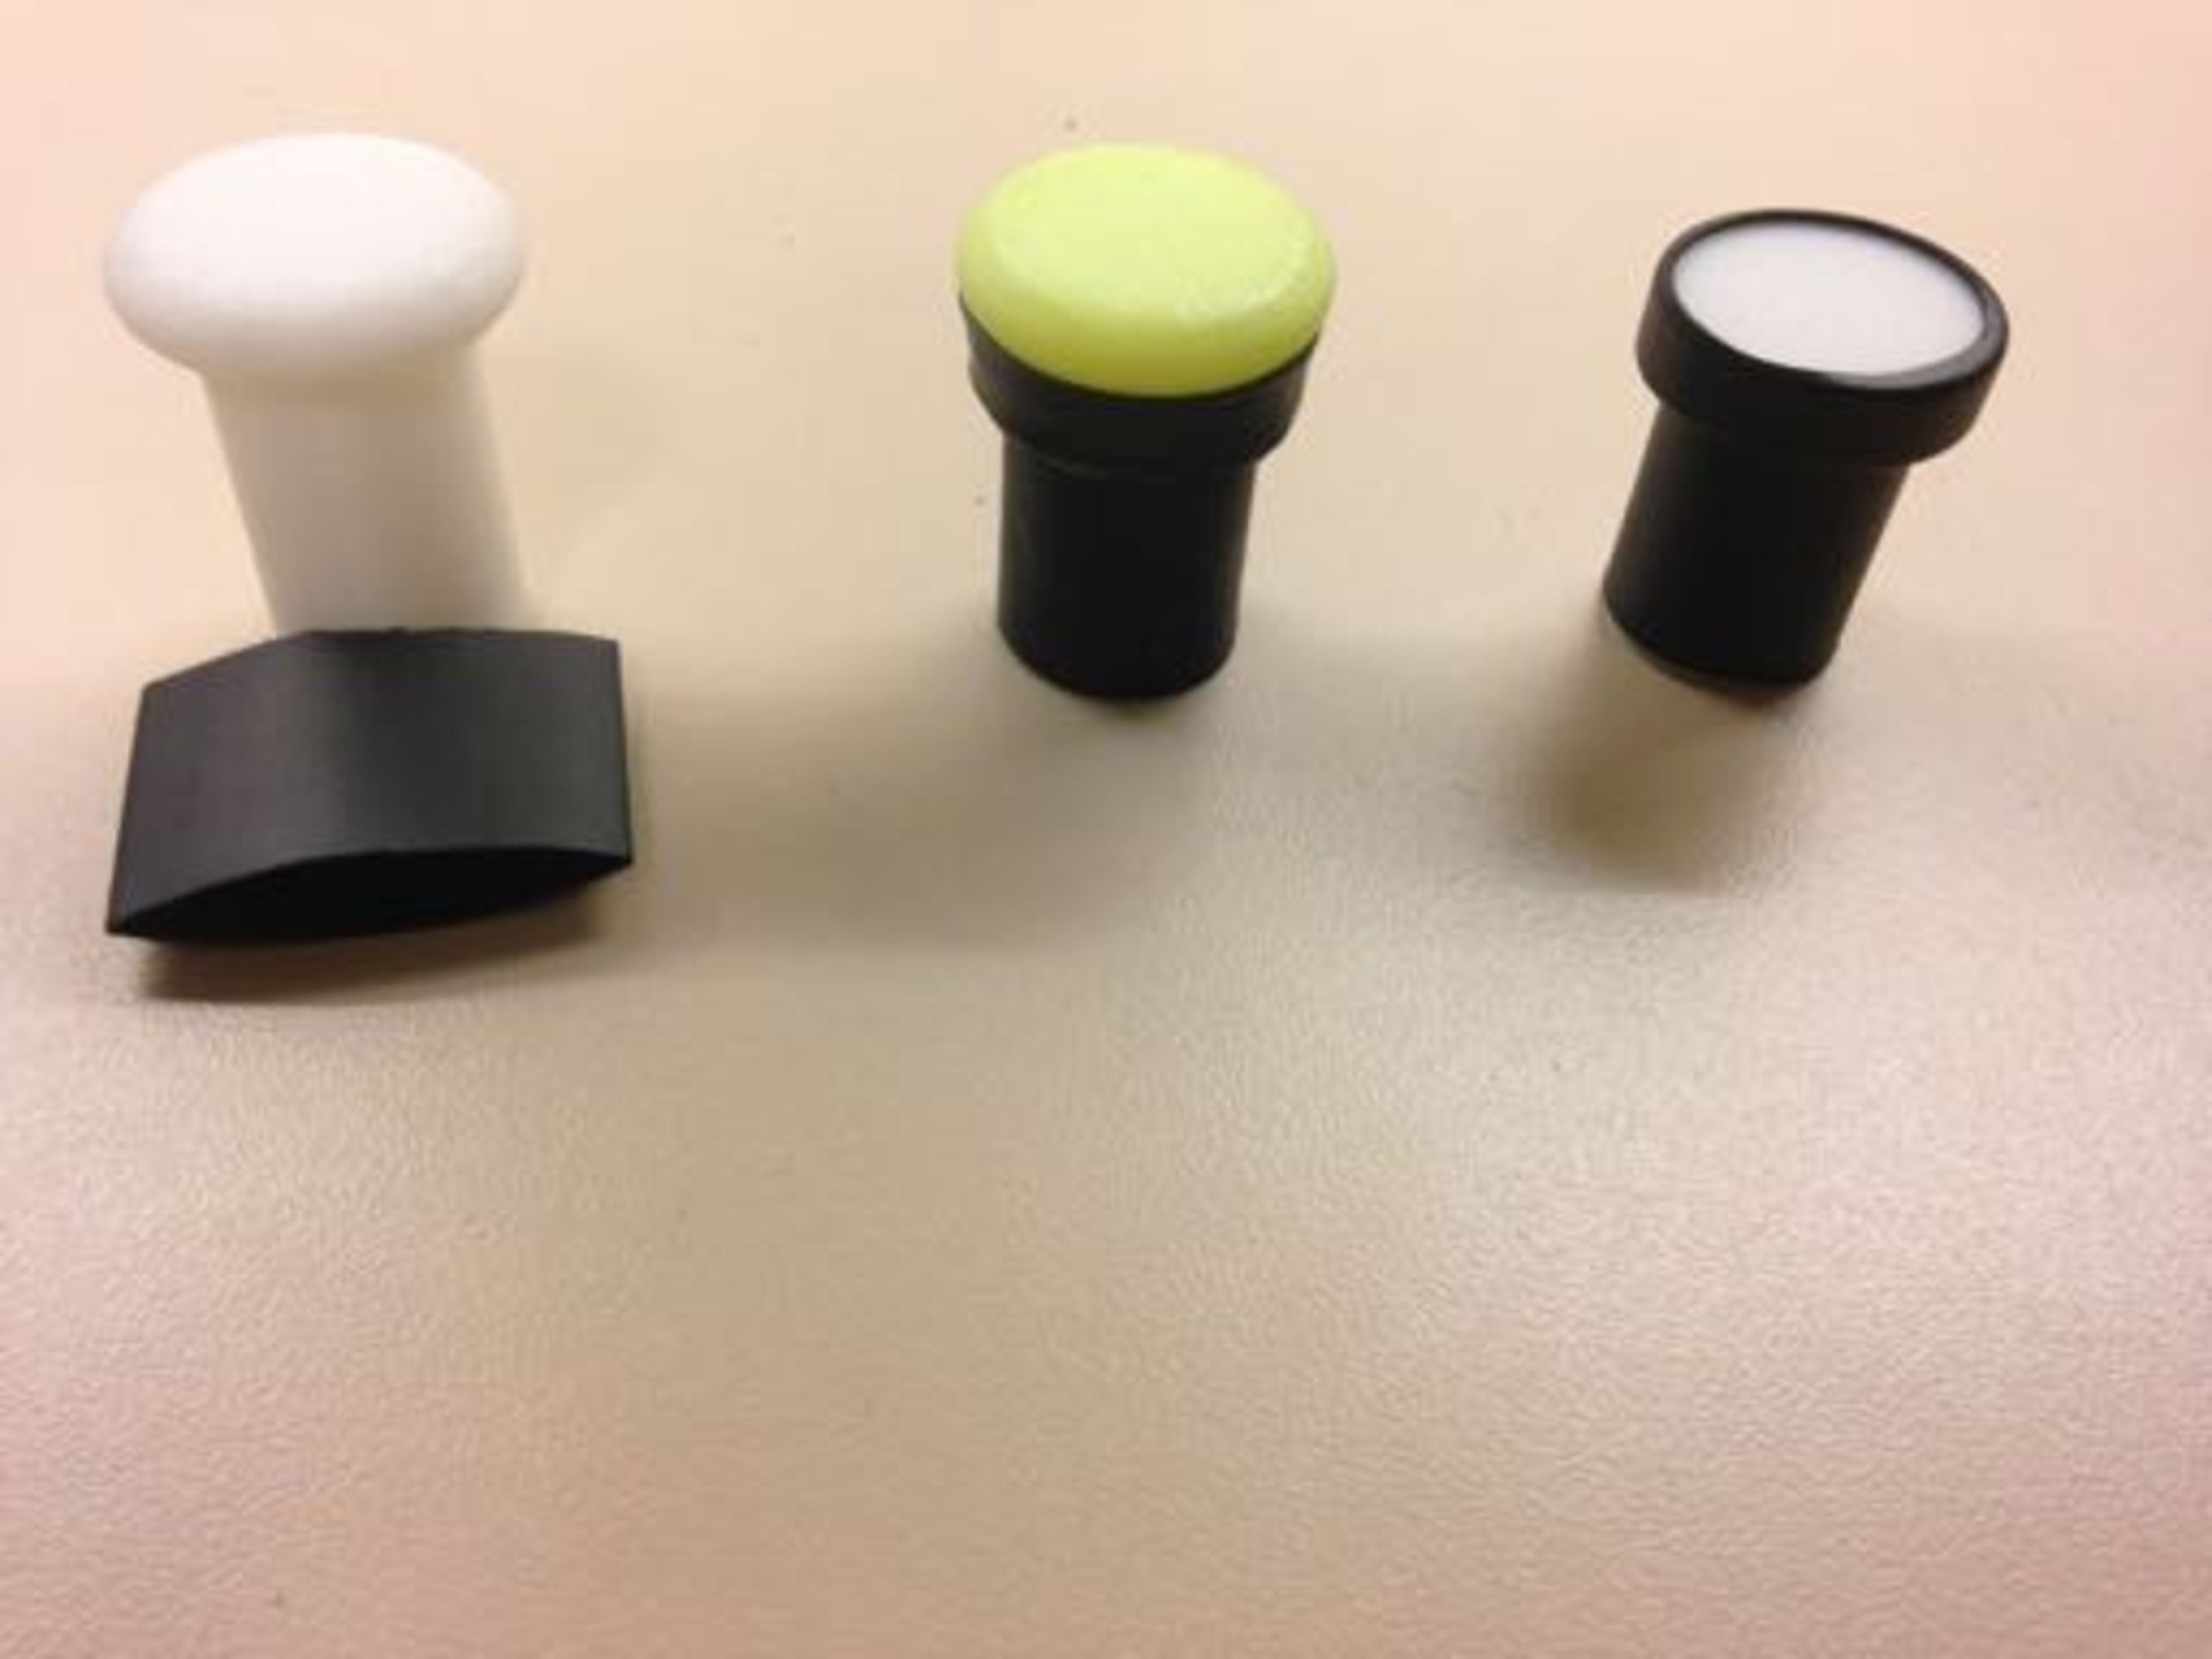
\includegraphics[width=3mm]{./figures/pinions.pdf}}
\item Place the pinion on the shaft of the motor. If this assembly is not tight enough the pinion can fall during the operation. 
\zoombox{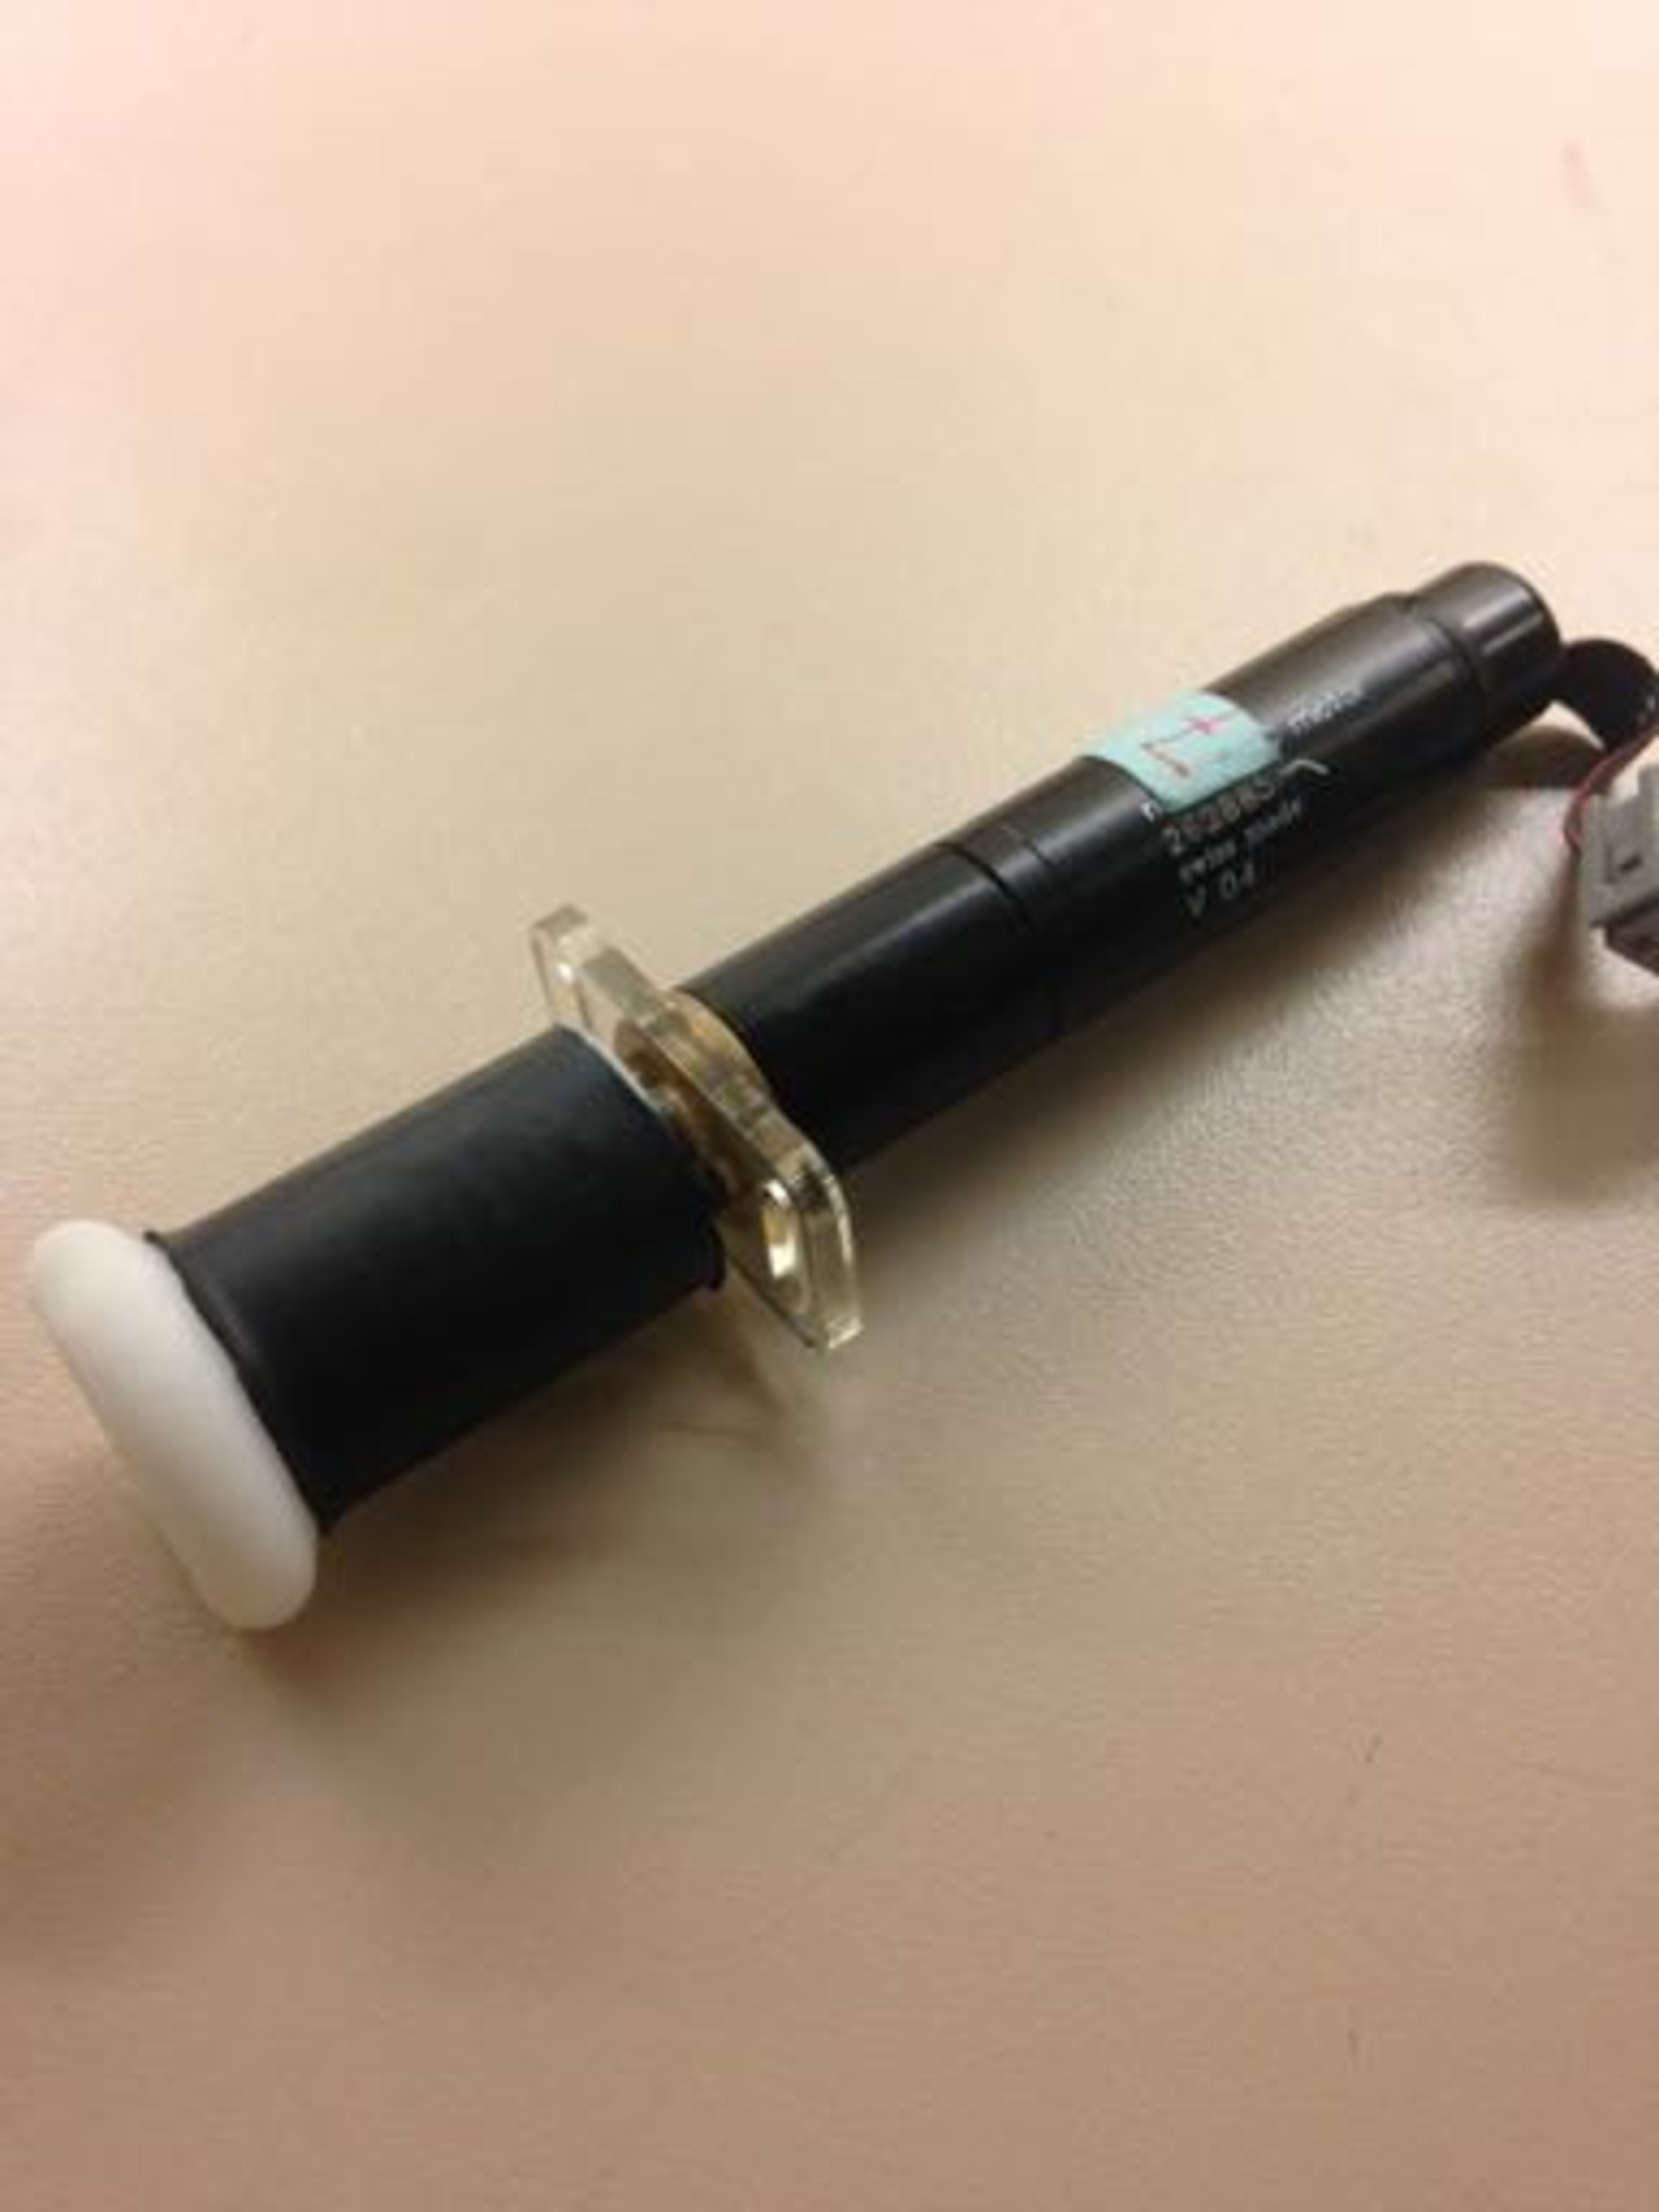
\includegraphics[width=3mm]{./figures/motor_pinion.pdf}}
\item Screw the motor holder on the base. The motor holder should be in front of the face.
\zoombox{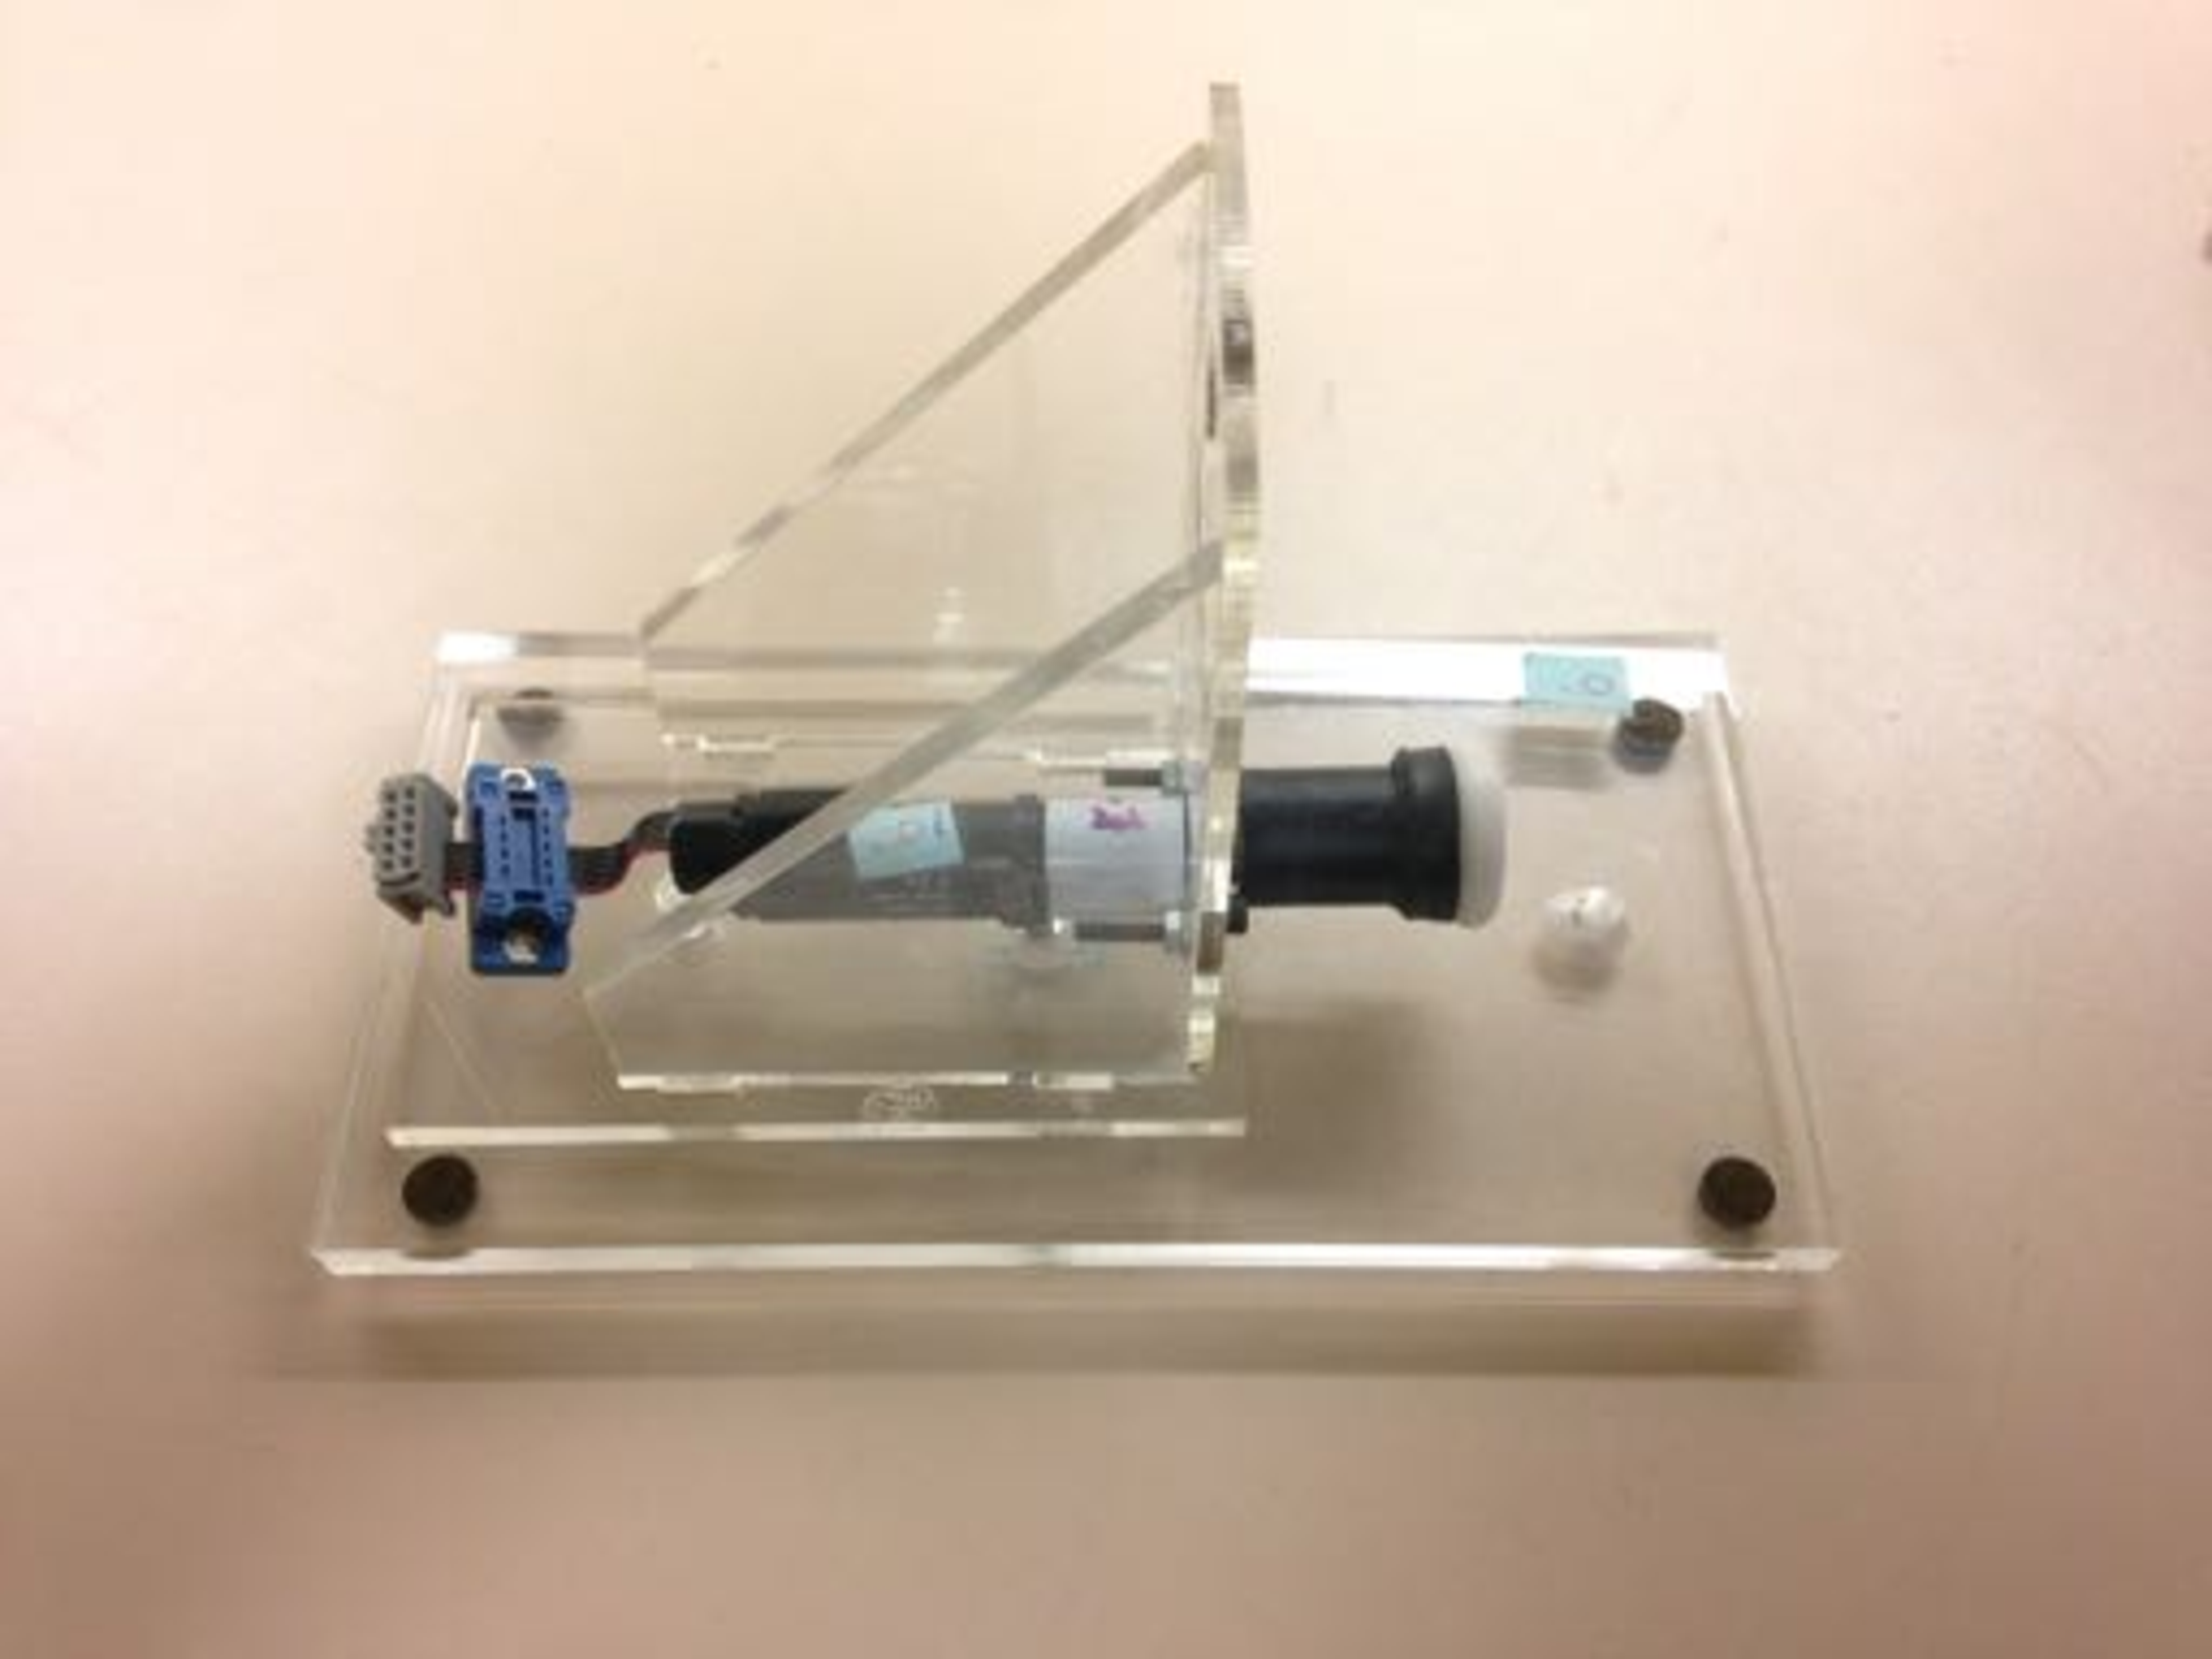
\includegraphics[width=3mm]{./figures/motor_base.pdf}}
\item The height adjustment of the motor should calibrated. Pinion should exert just enough force on pulley to provide desired friction.
\end{enumerate}
\end{itemize}
\scriptsize
\vspace{-2mm}
The end product of this section should look like
\hspace{2mm}
\zoombox{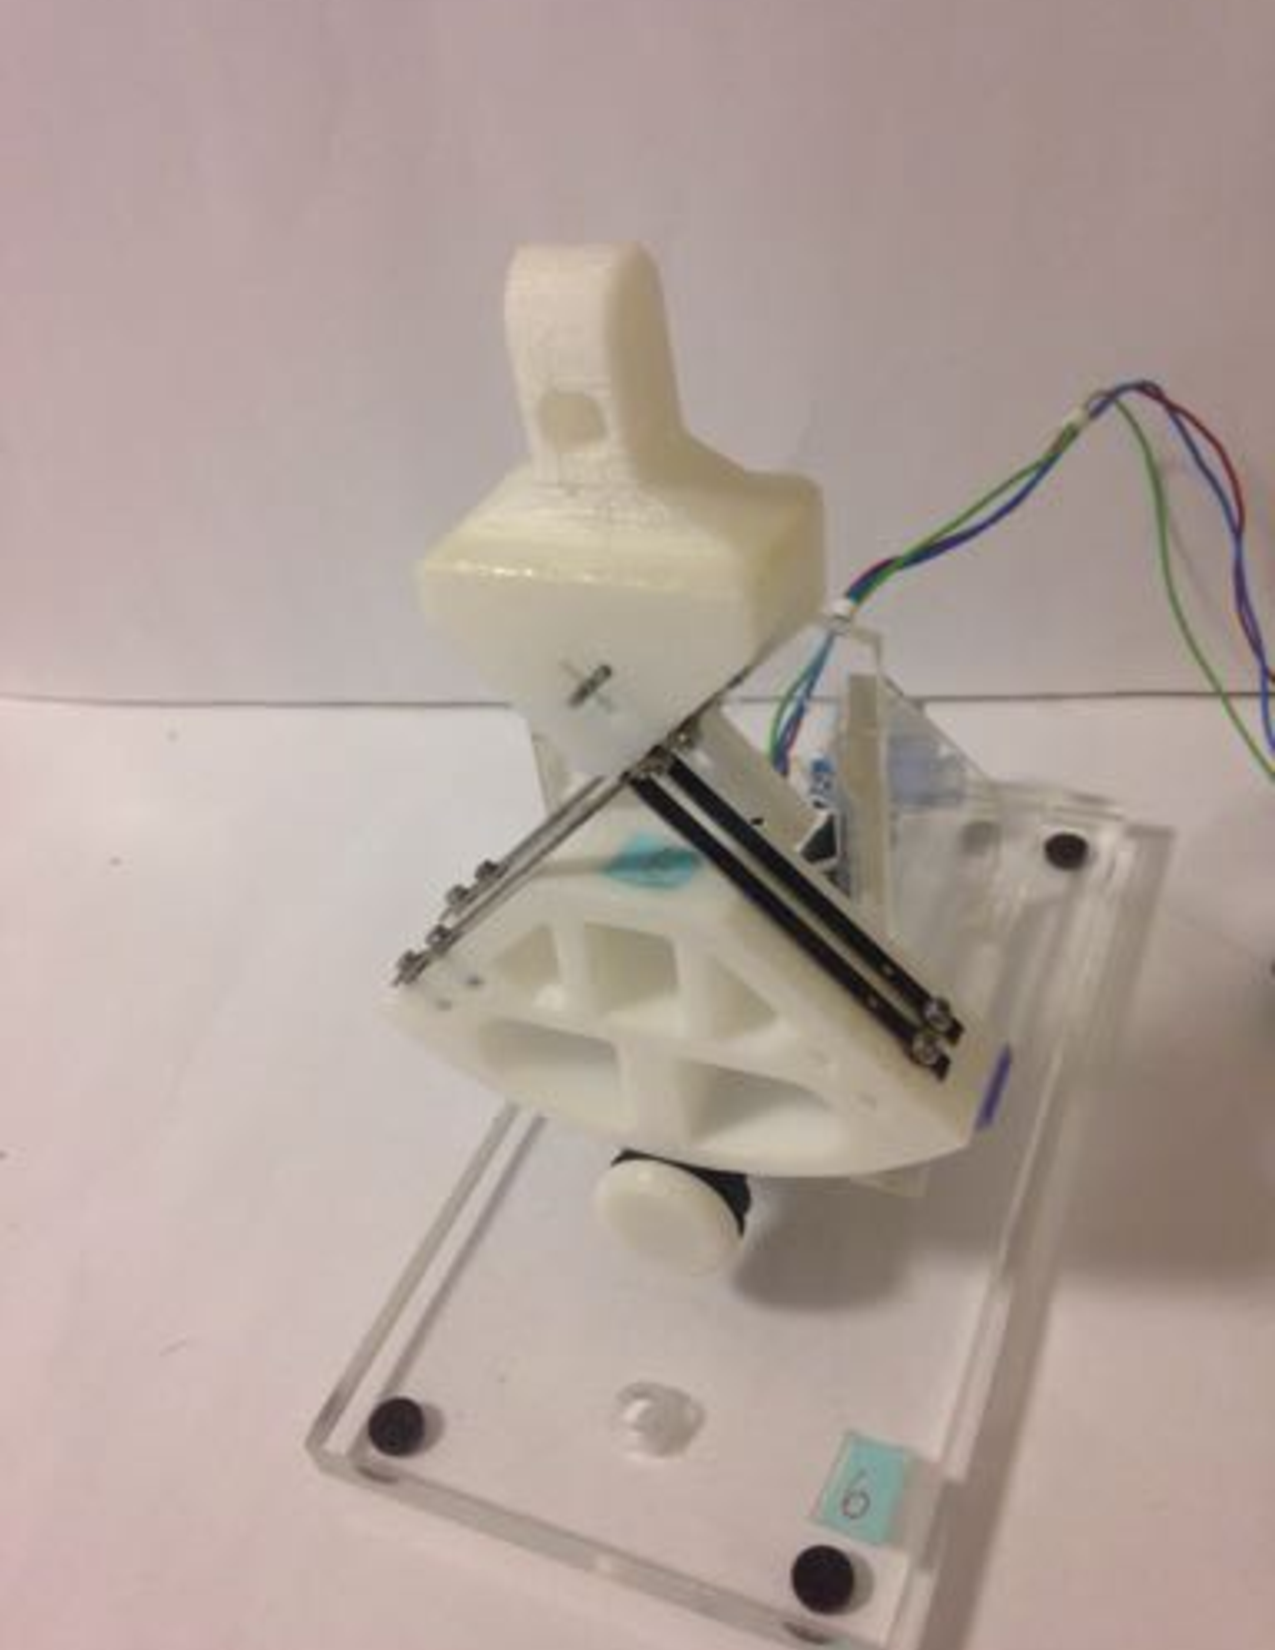
\includegraphics[width=2mm]{./figures/base_capstan.pdf}}
\end{frame}

\begin{frame}[t]{Creating the PCB}
\begin{itemize} 
\item Components
\begin{itemize} \scriptsize
\item Pressed/Printed Circuit Board
\item 2x Resistors
\item DRV 8801 Driver
\item Benchtop drill press
\item 3 pin PCB connector
\item 4 pin PCB connector
\item Single and double row 1" female pin headers
\end{itemize}
\item Procedure
\begin{enumerate} \scriptsize
\item Using the Eagle files press the raw circuit board
\zoombox{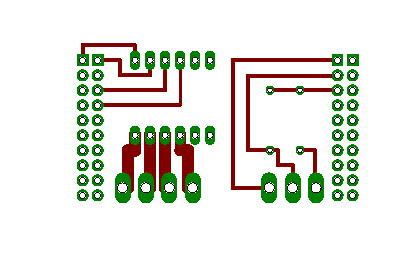
\includegraphics[width=3mm]{./figures/PCB_manu.pdf}}
\item Drill through the required holes
\zoombox{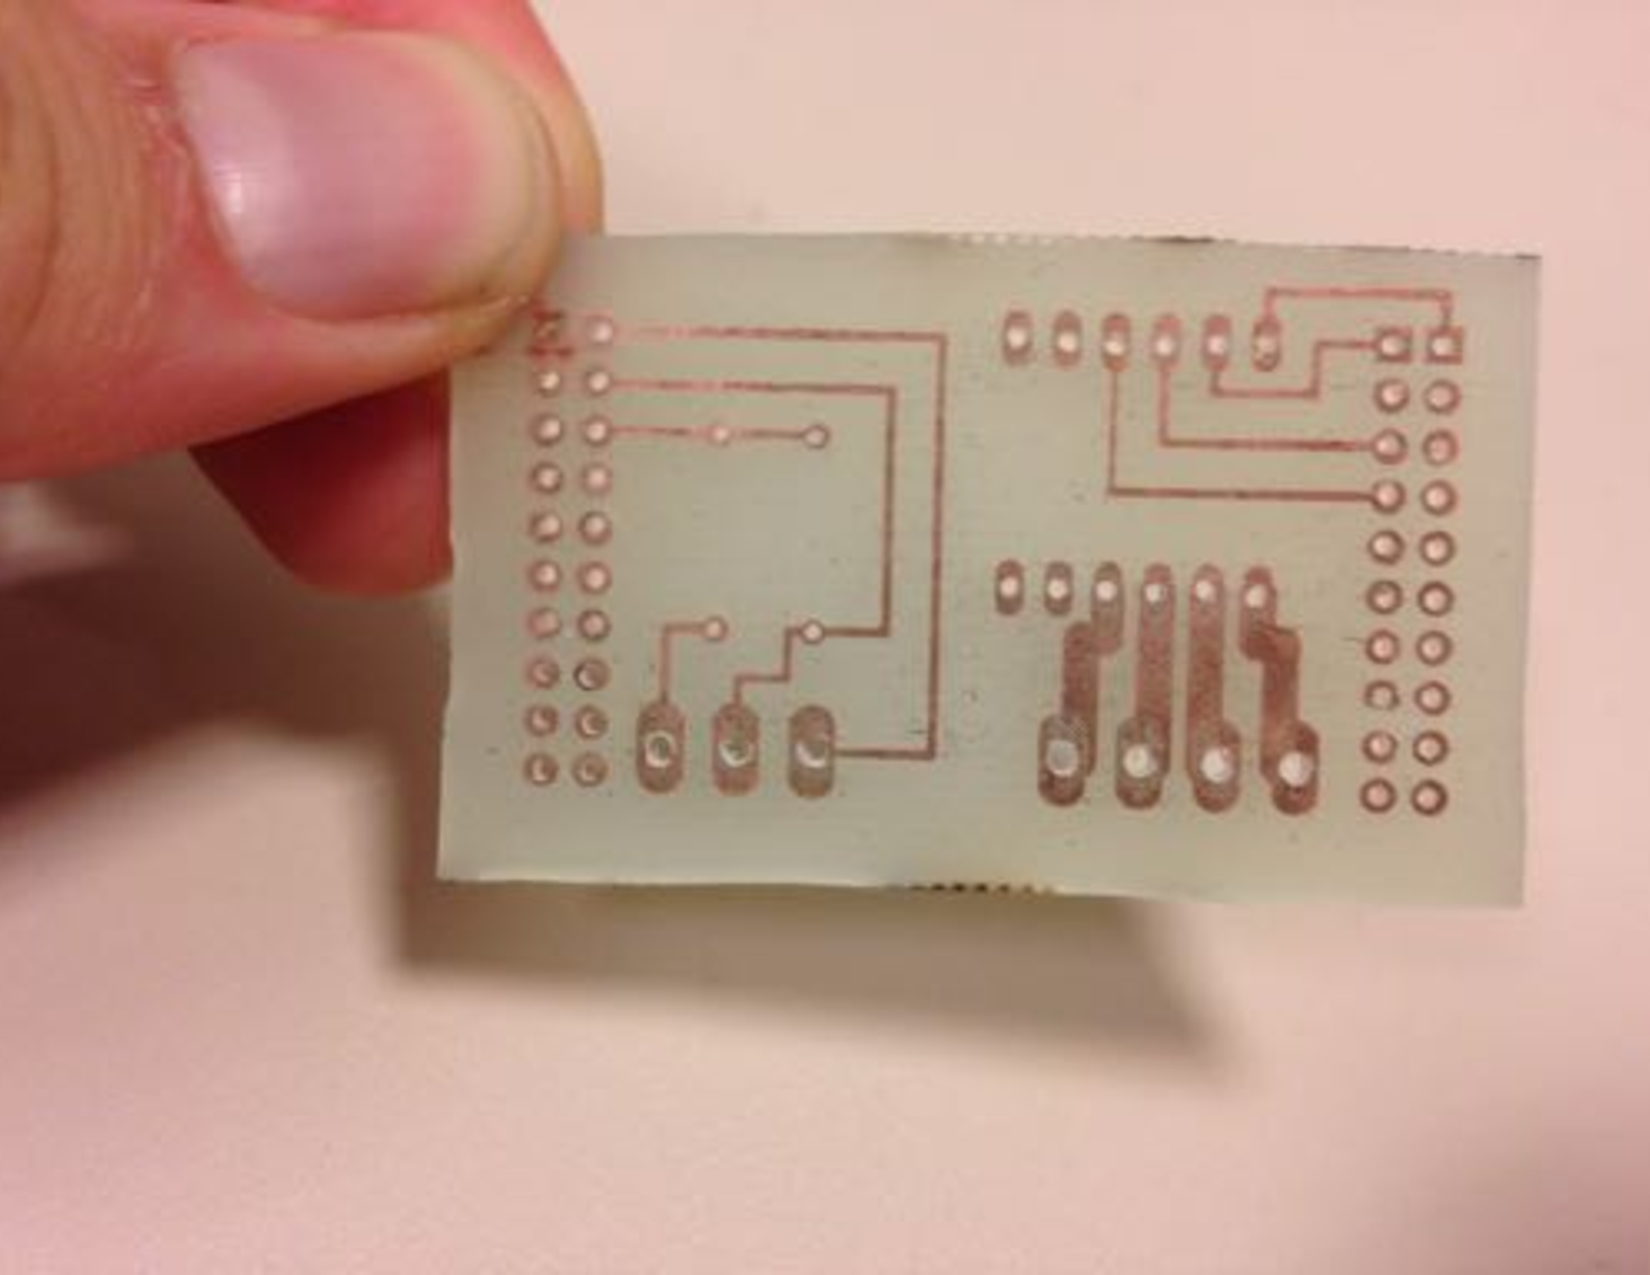
\includegraphics[width=3mm]{./figures/pcb_naked.pdf}} (Note that the when printed the apperance is reflected around vertical axis)
\item First solder the legs (male pin headers) of DRV8801 on the PCB, then solder the DRV8801.
\item Selection of resistors for the voltage to drop the voltage from 0-5V to 0-≤3.3 V range.  1.5 and 2.7(green one) kOhm were used but can vary. Make sure the resistance values are high enough though.
\item Place in and solder the other required components as seen in the pictures. 
\zoombox{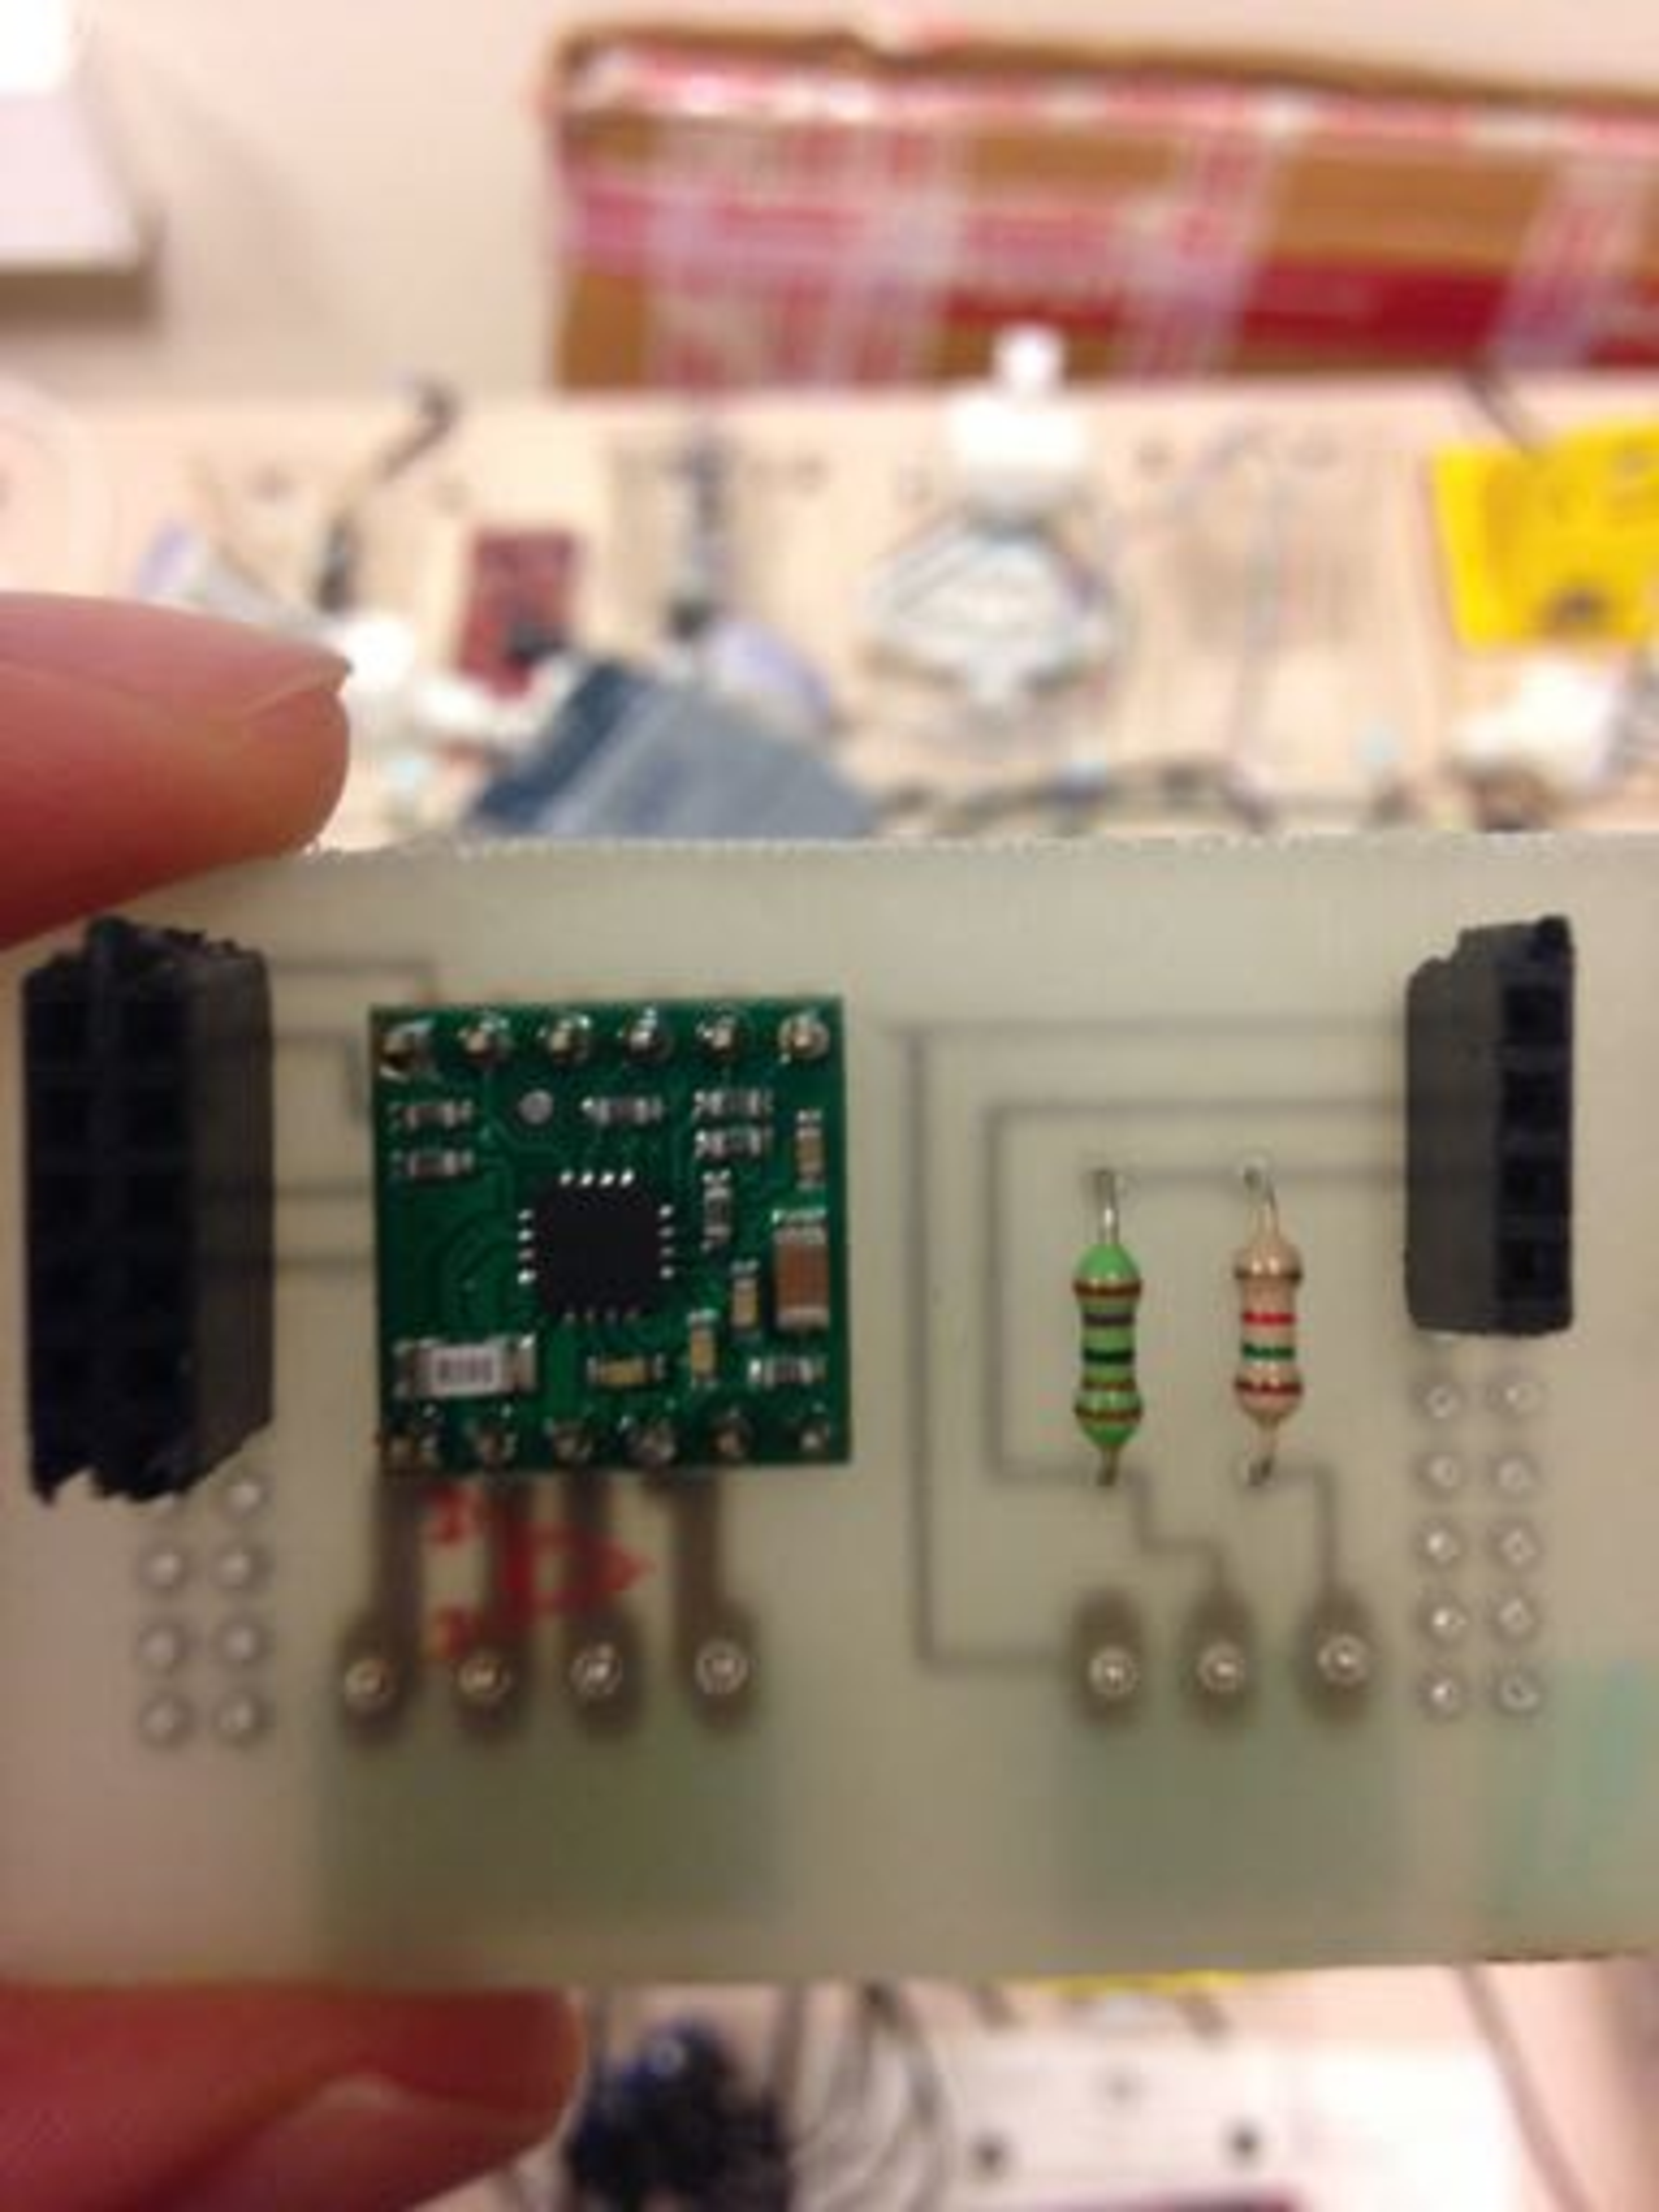
\includegraphics[width=3mm]{./figures/pcb_front.pdf}}
\zoombox{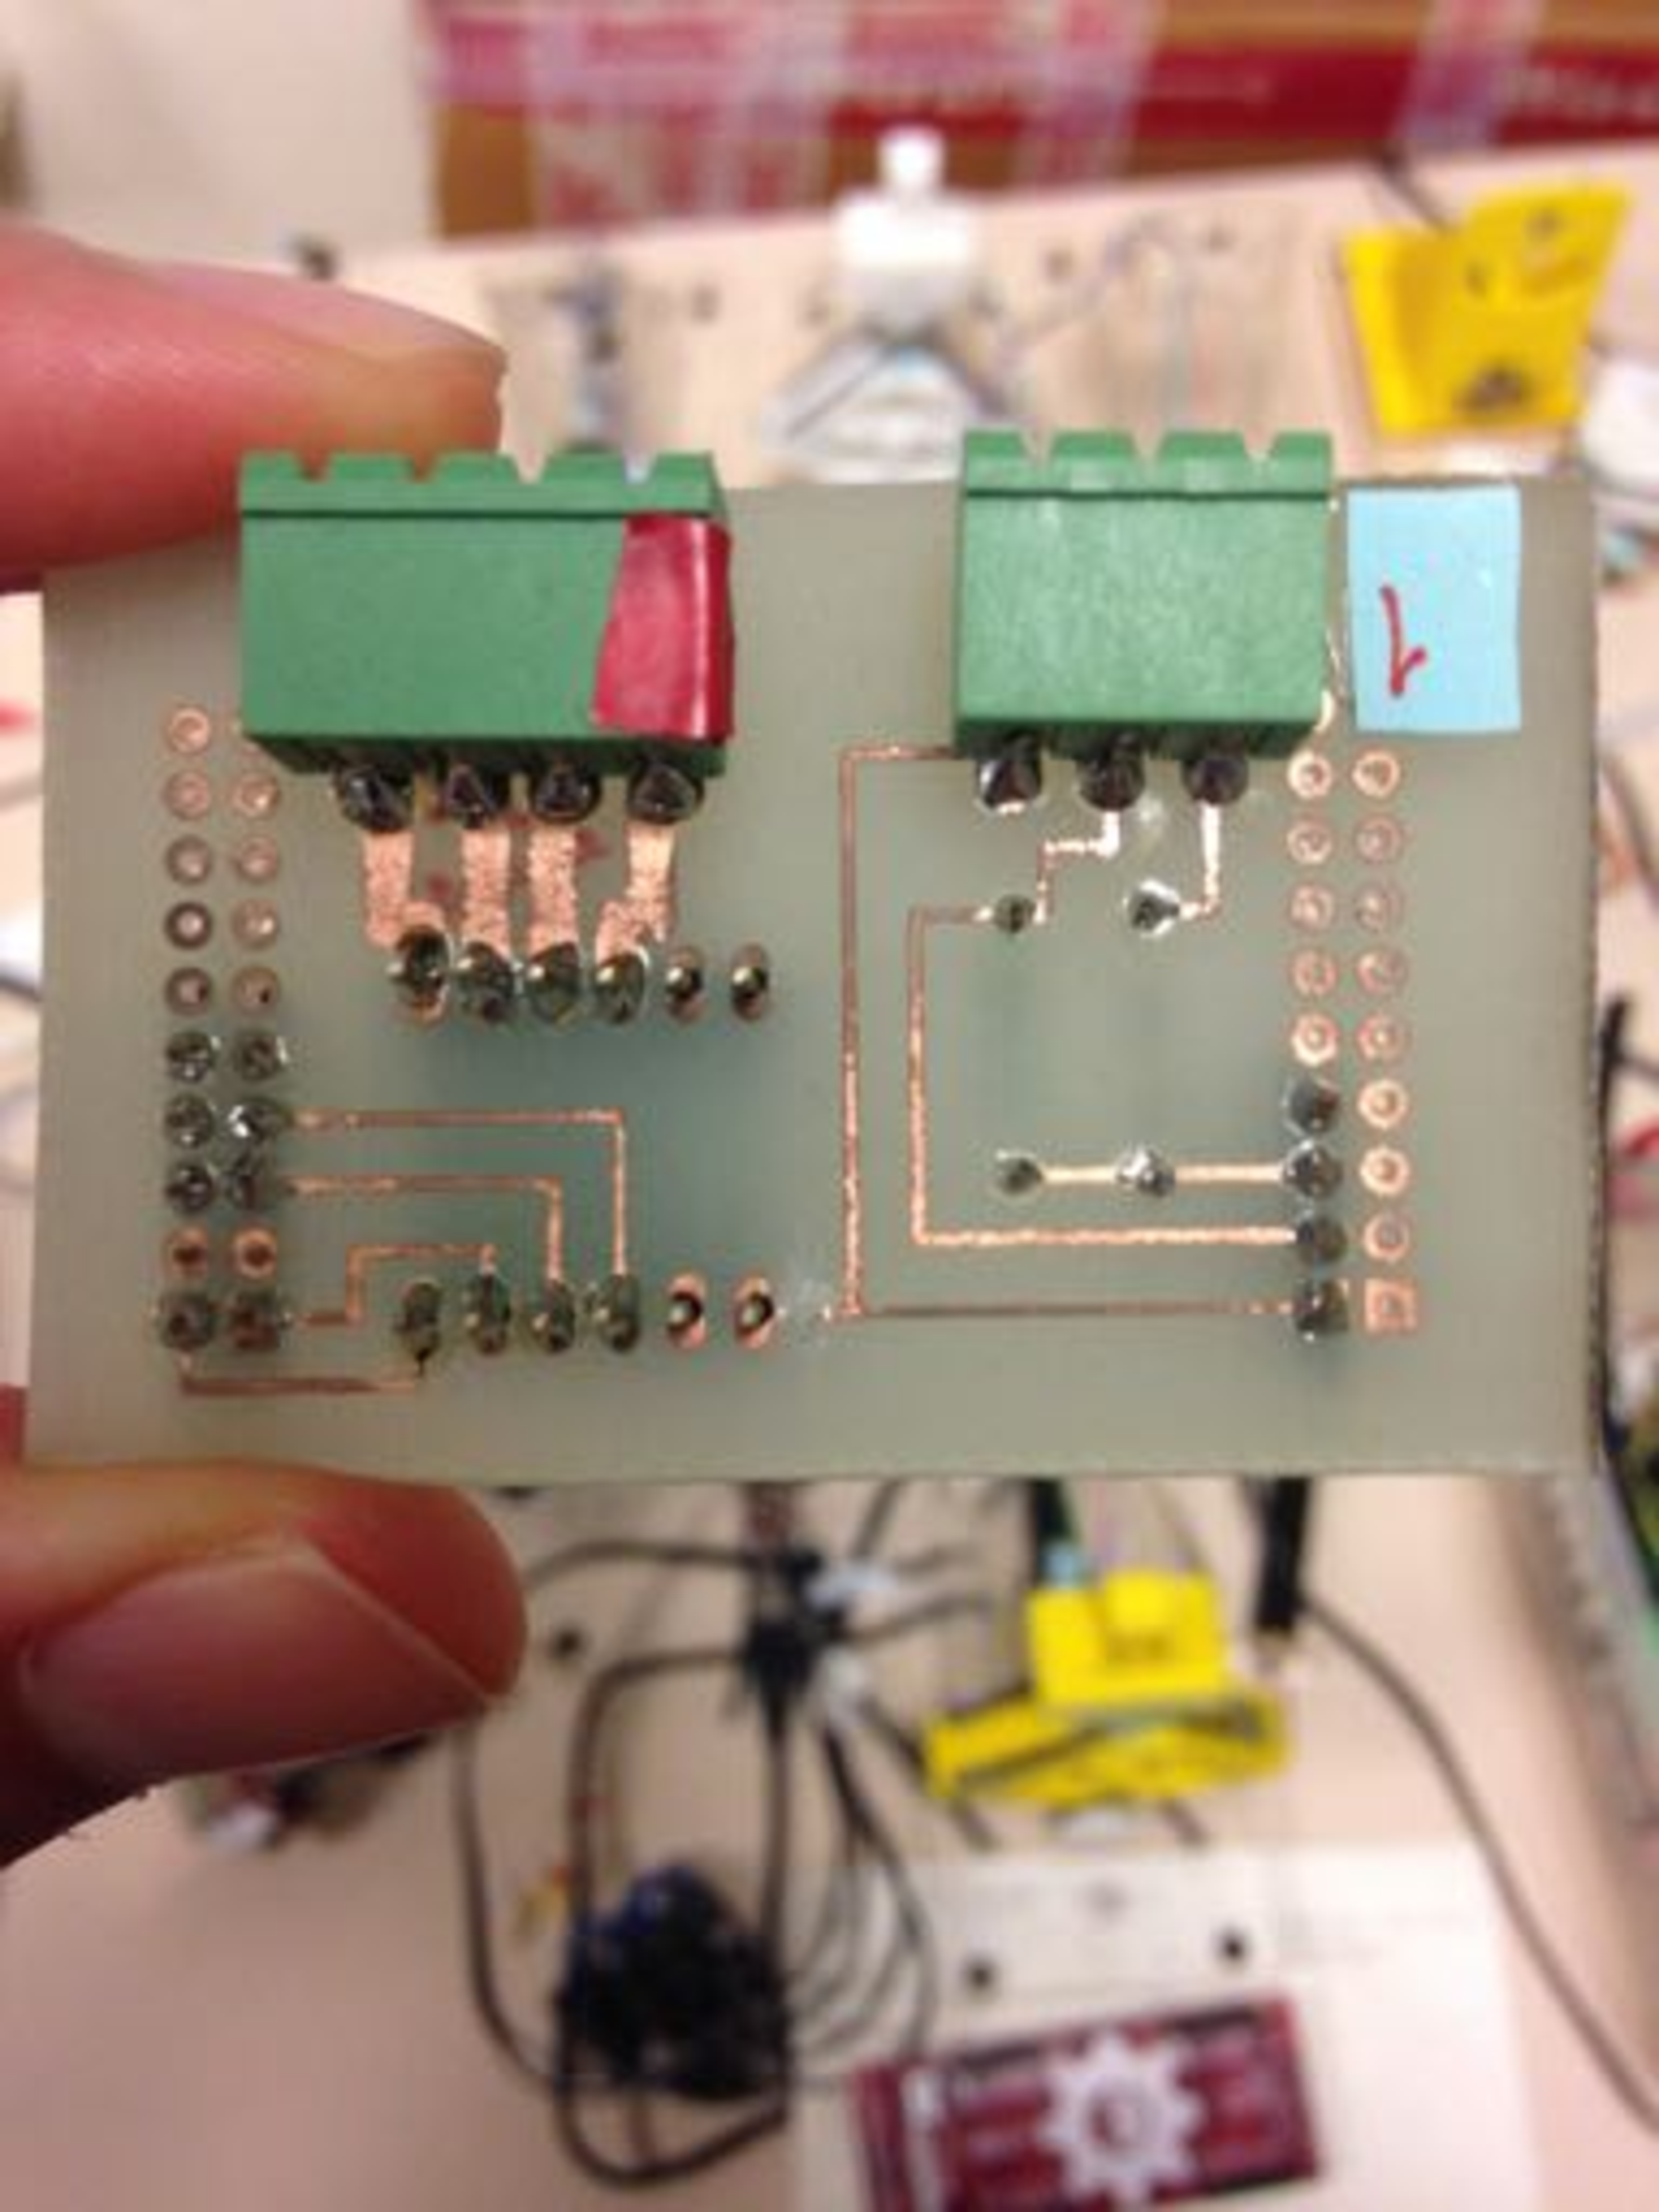
\includegraphics[width=3mm]{./figures/pcb_back.pdf}}
\end{enumerate}
\end{itemize}
\end{frame}

\begin{frame}[t]{Electronic Assembly}
\begin{itemize} 
\item Components
\begin{itemize} \scriptsize
\item PCB
\item TI F28069M Microcontroller
\item HandsOn SEA mechanical assembly
\item Jumper wires
\item 24 V power supply
\item Screw driver
\end{itemize}
\item Procedure (please refer to the pictures for each step)
\begin{enumerate} \scriptsize
\item Place the PCB on the microcontroller
\zoombox{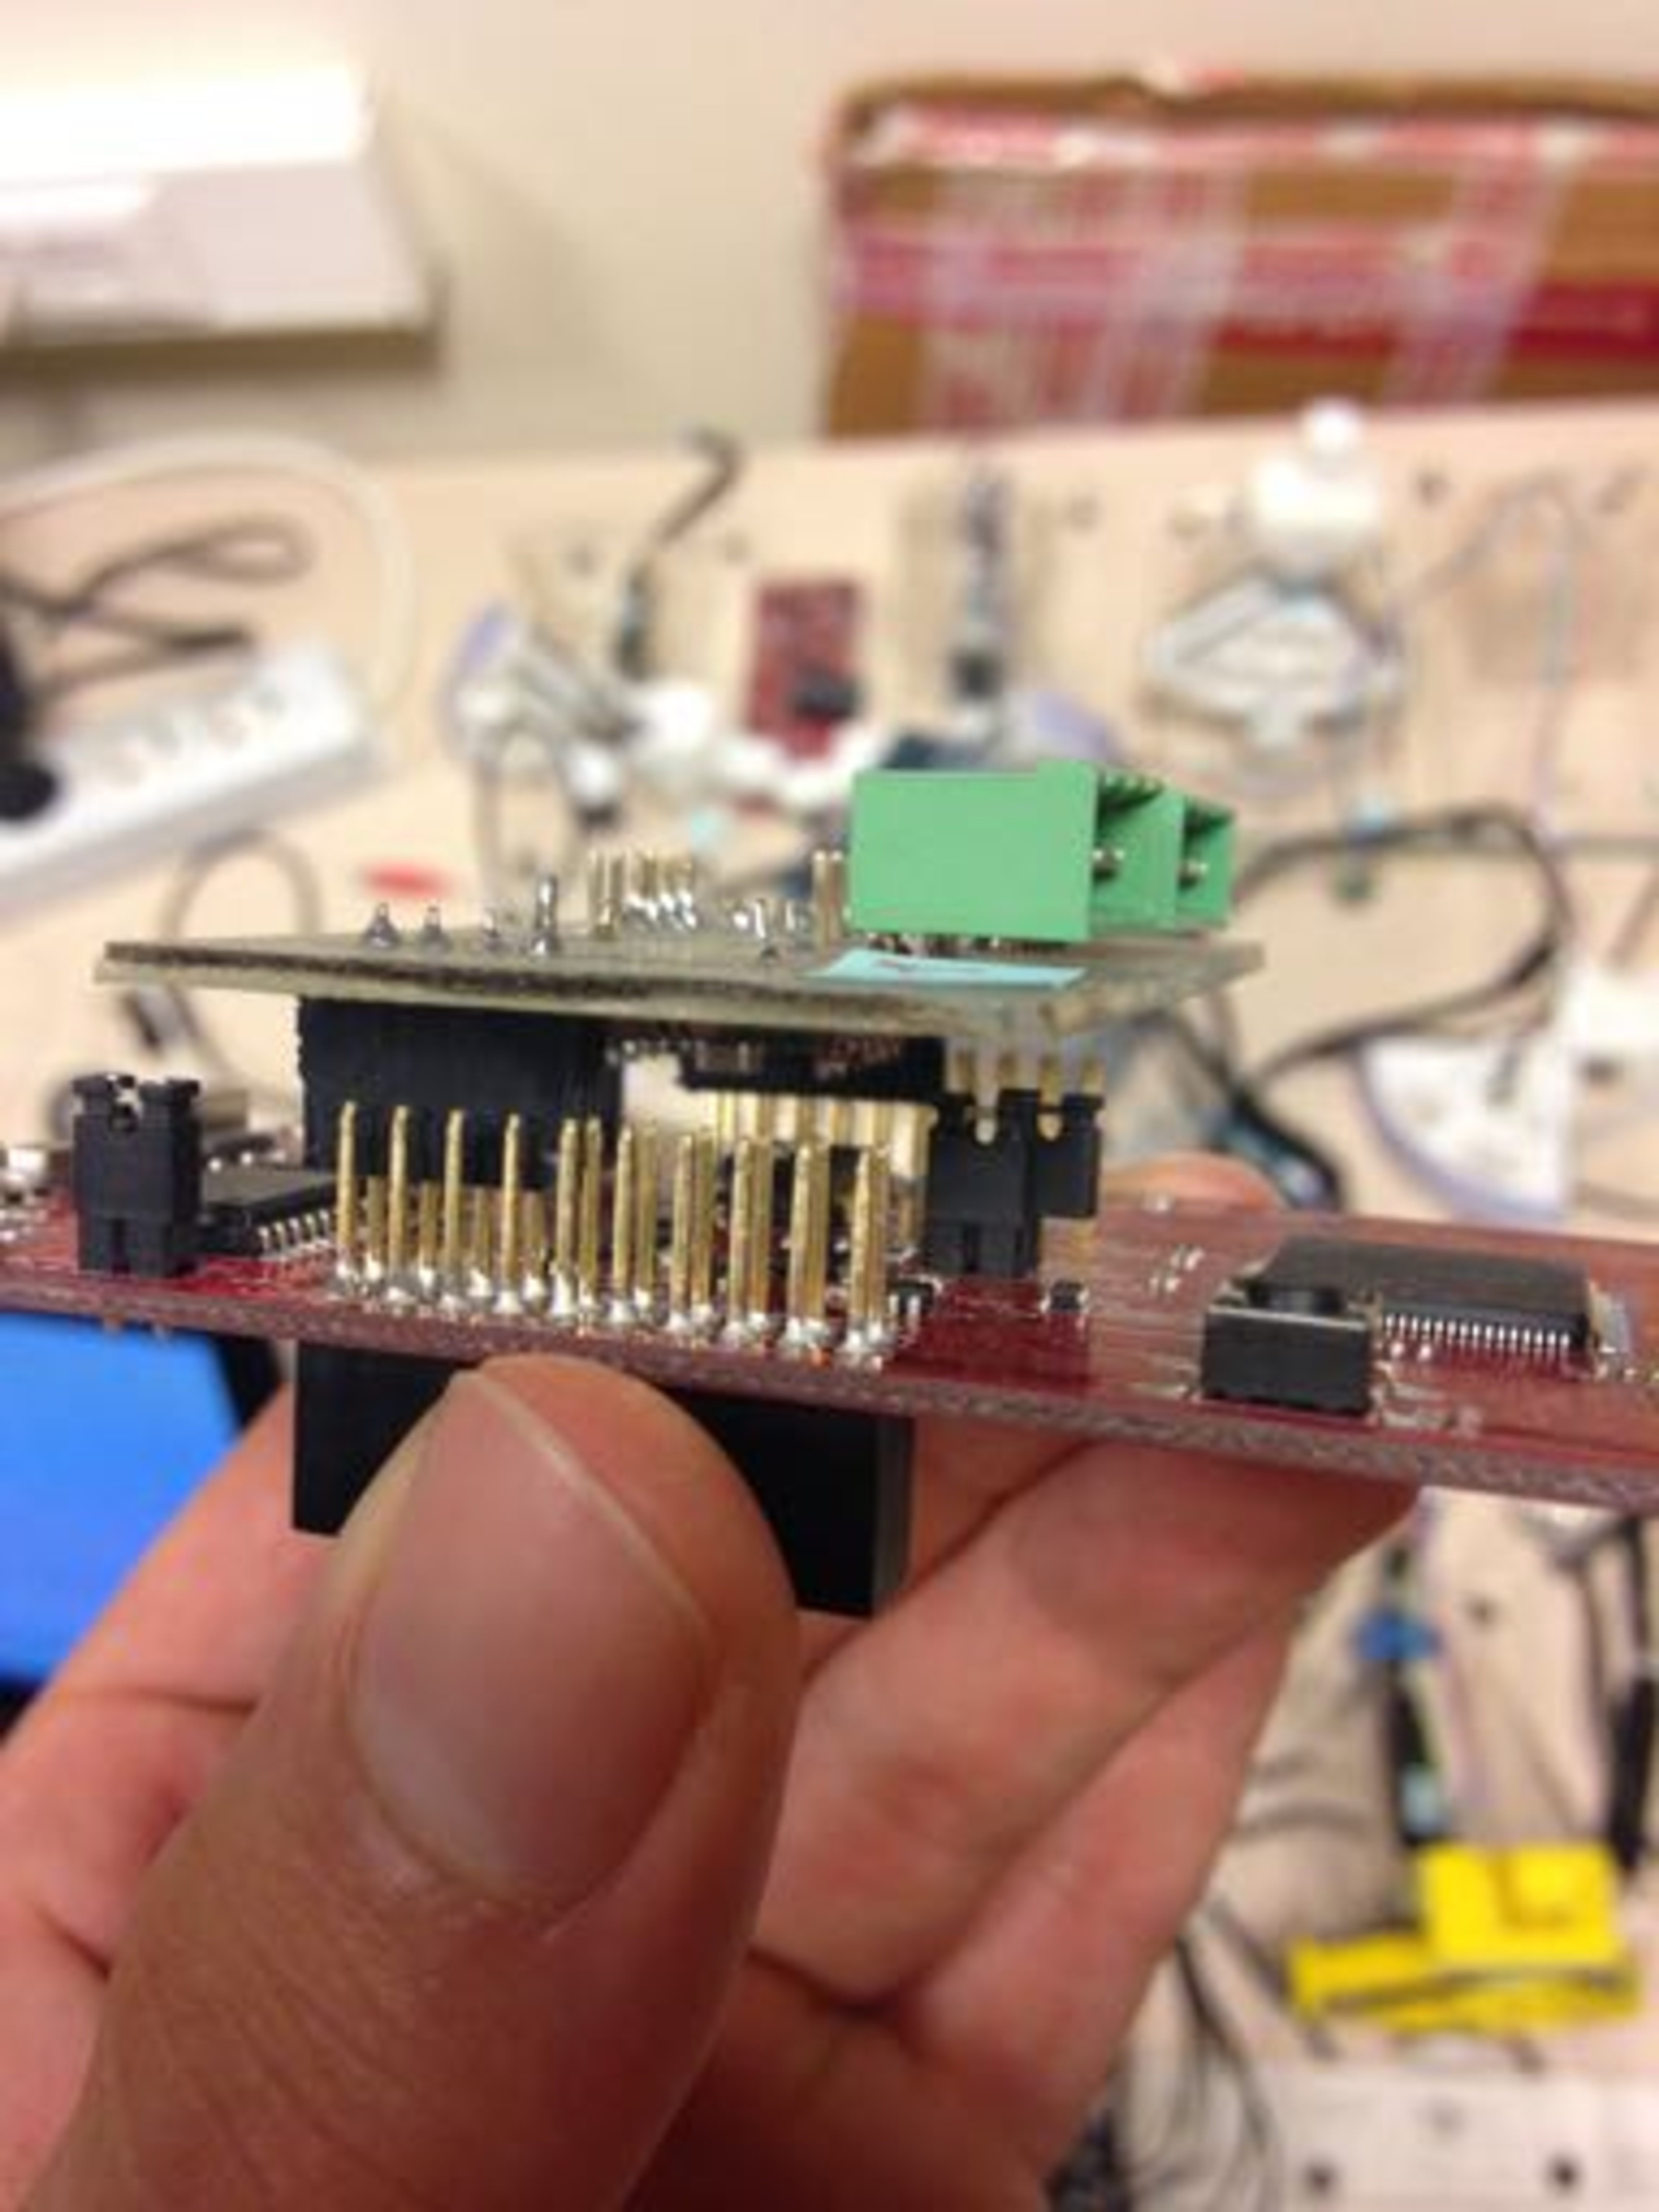
\includegraphics[width=3mm]{./figures/pcb_mount.pdf}}
\zoombox{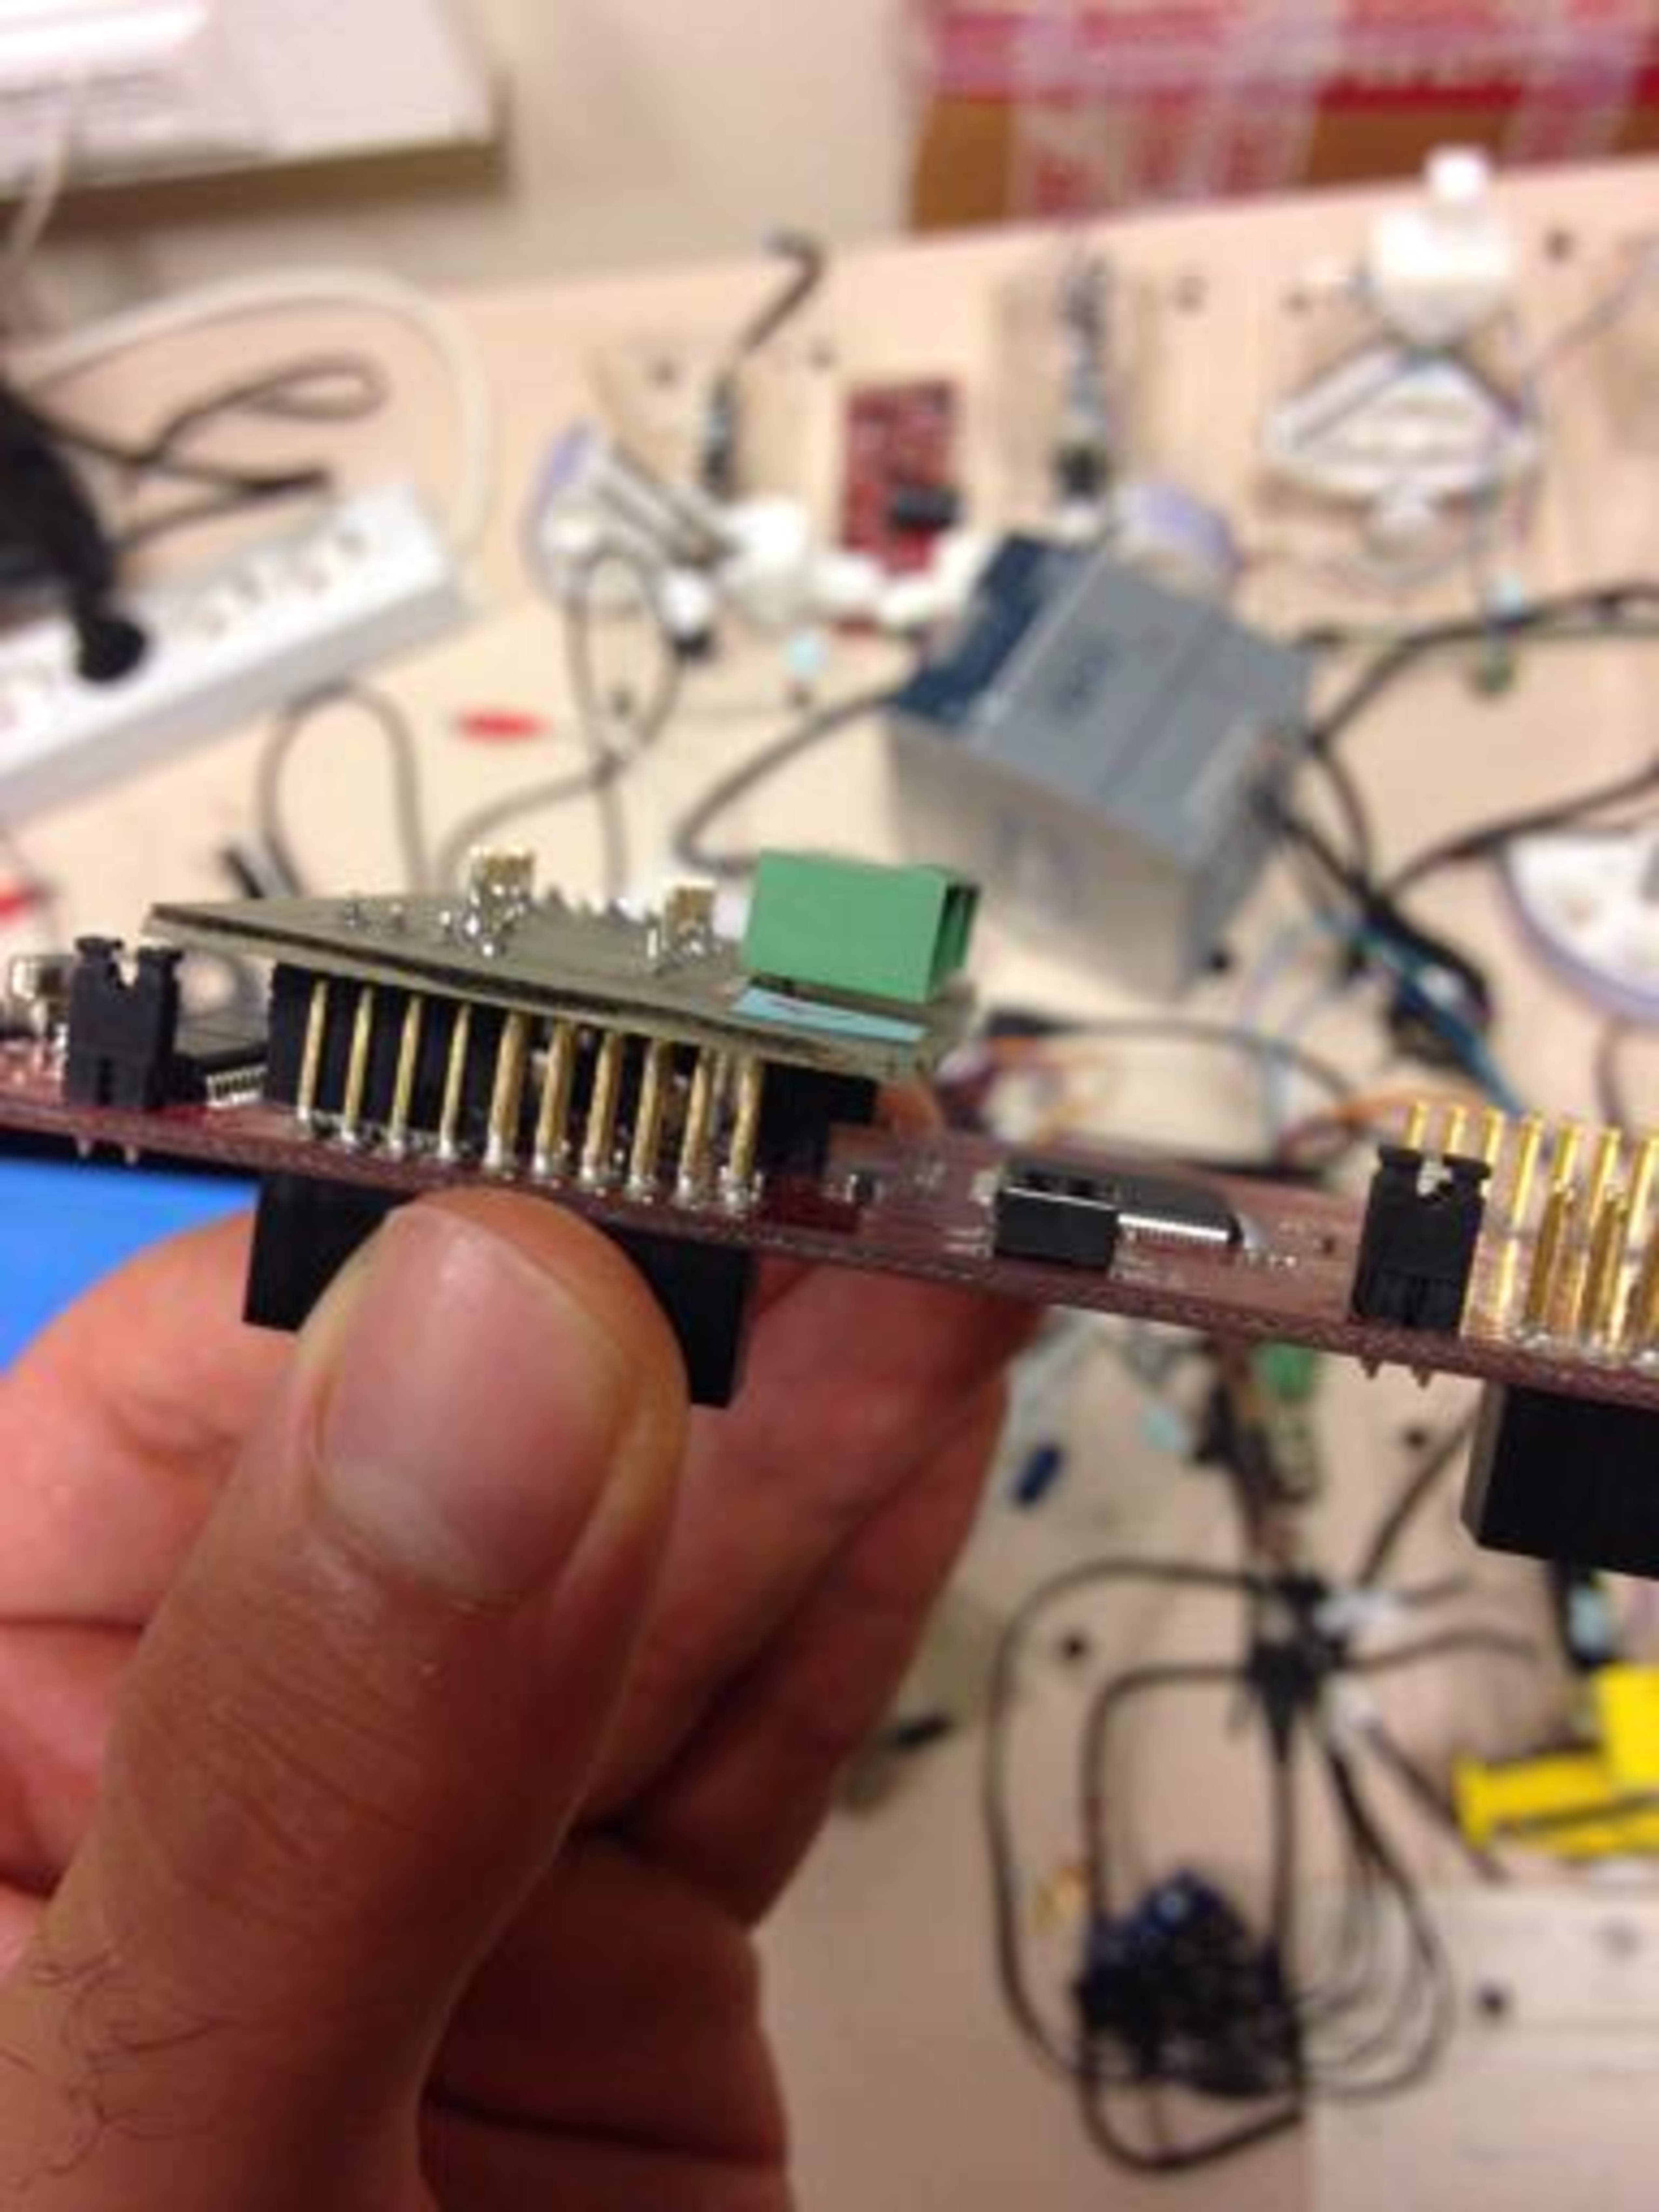
\includegraphics[width=3mm]{./figures/pcb_mount2.pdf}}
\item Connect the hall effect sensor to 3 pin PCB connector
\zoombox{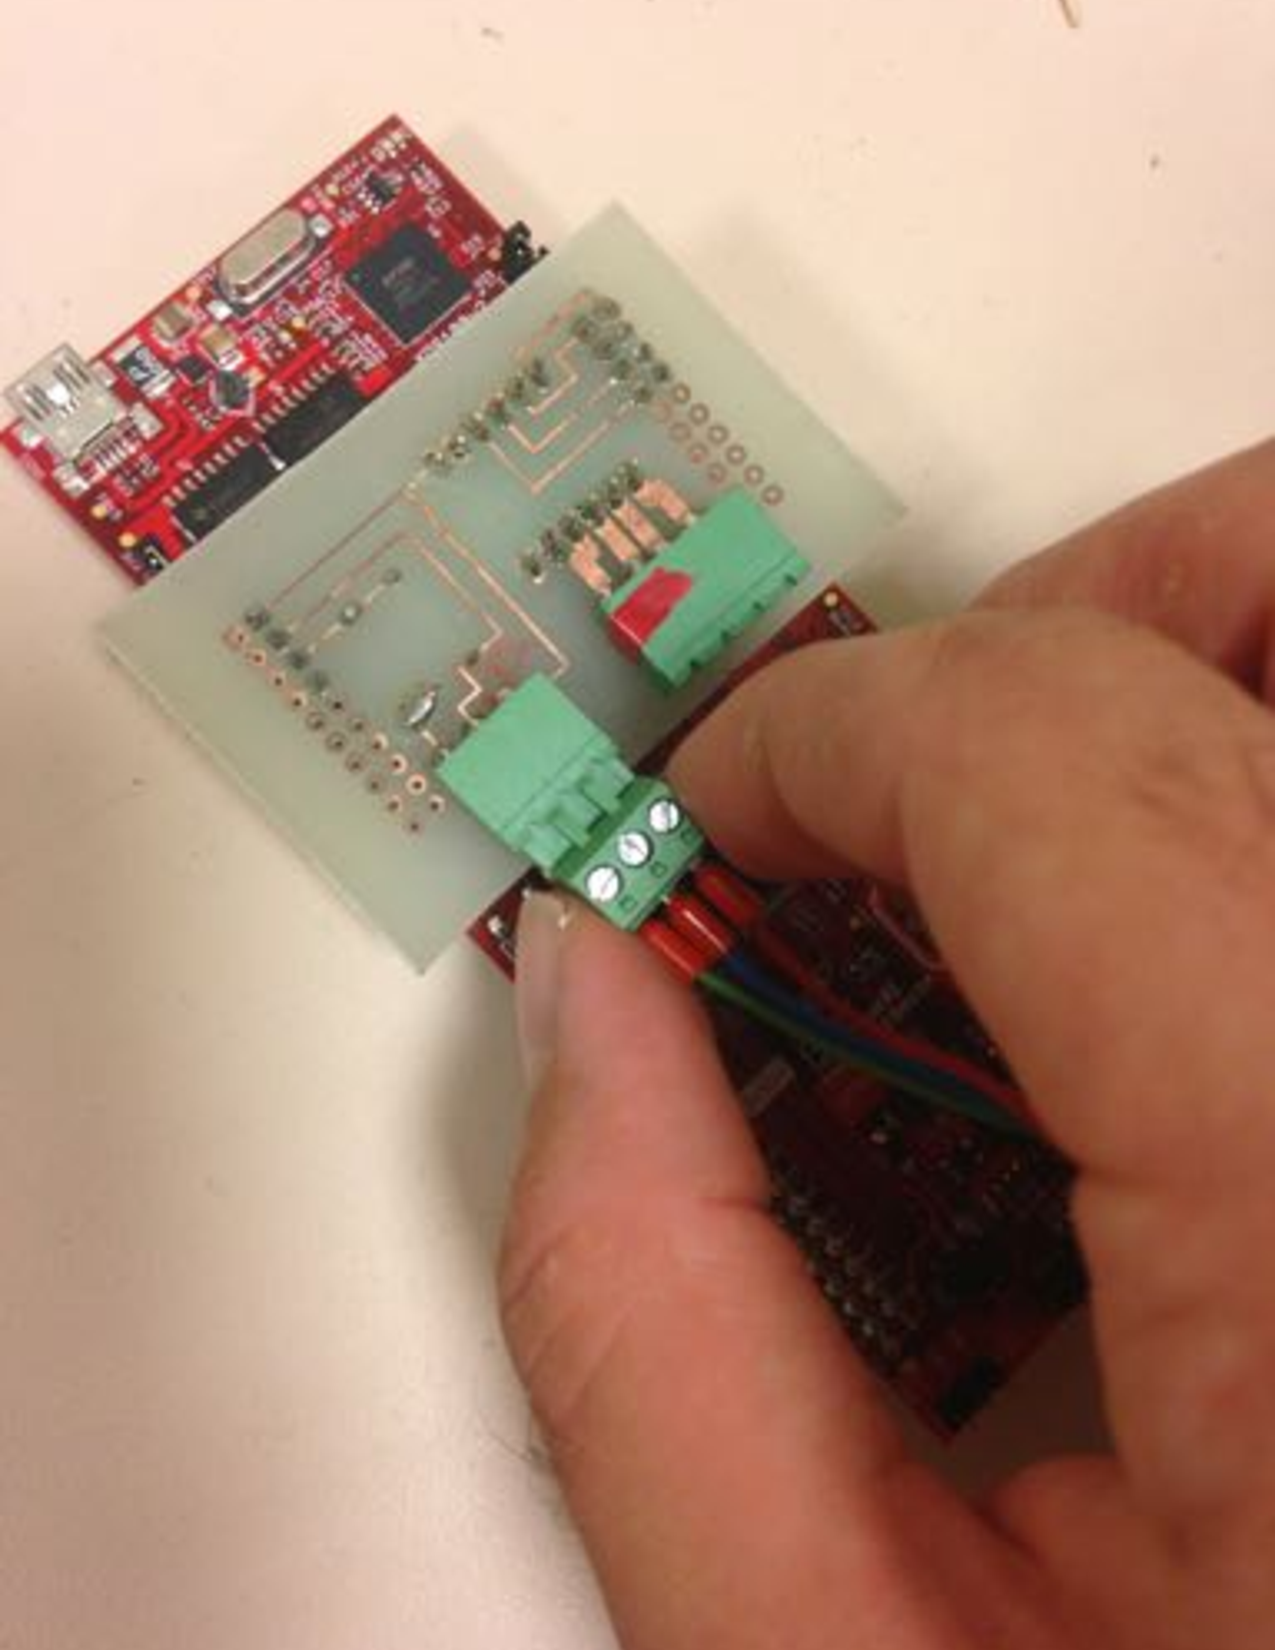
\includegraphics[width=3mm]{./figures/PCB_3pin.pdf}}
\item Plug in 6 male ends of female to male jumper wires on the motor's connector. Using different type of motor would of course change this step. 
\zoombox{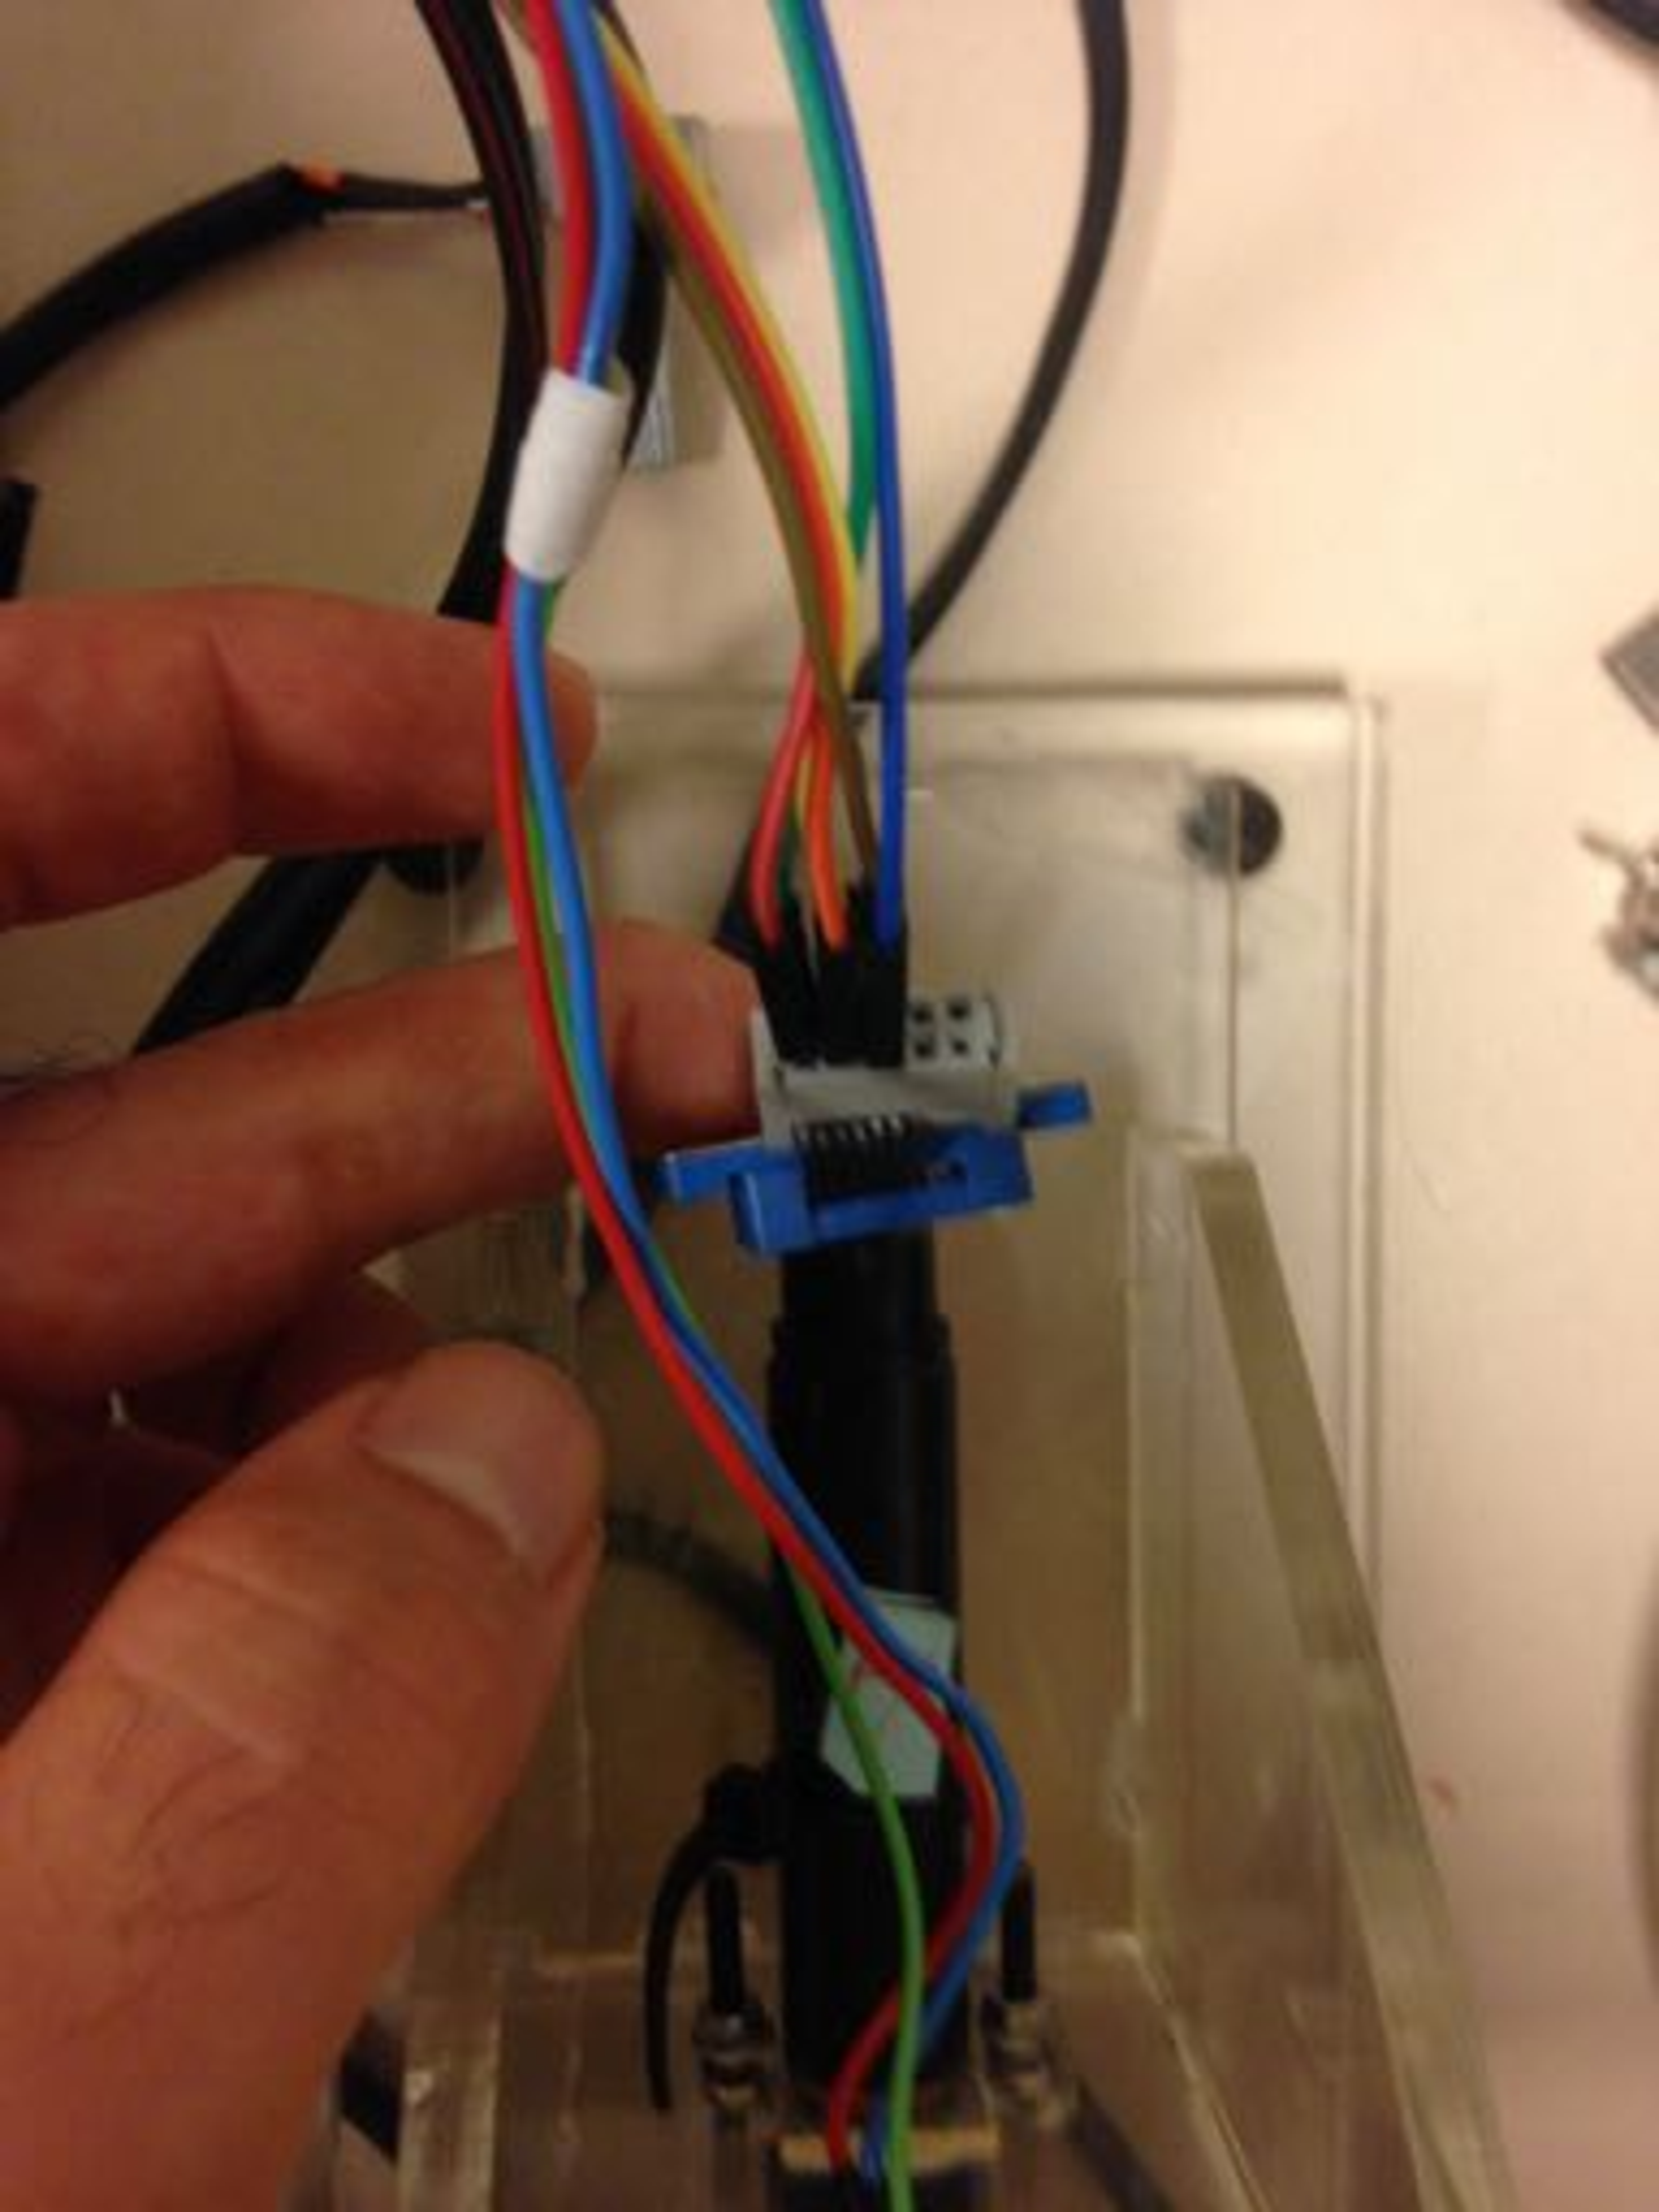
\includegraphics[width=3mm]{./figures/motor_wiring.pdf}}
\item Connect the power supply wires and the motor energy supply wires to 4 pin PCB connector.
\zoombox{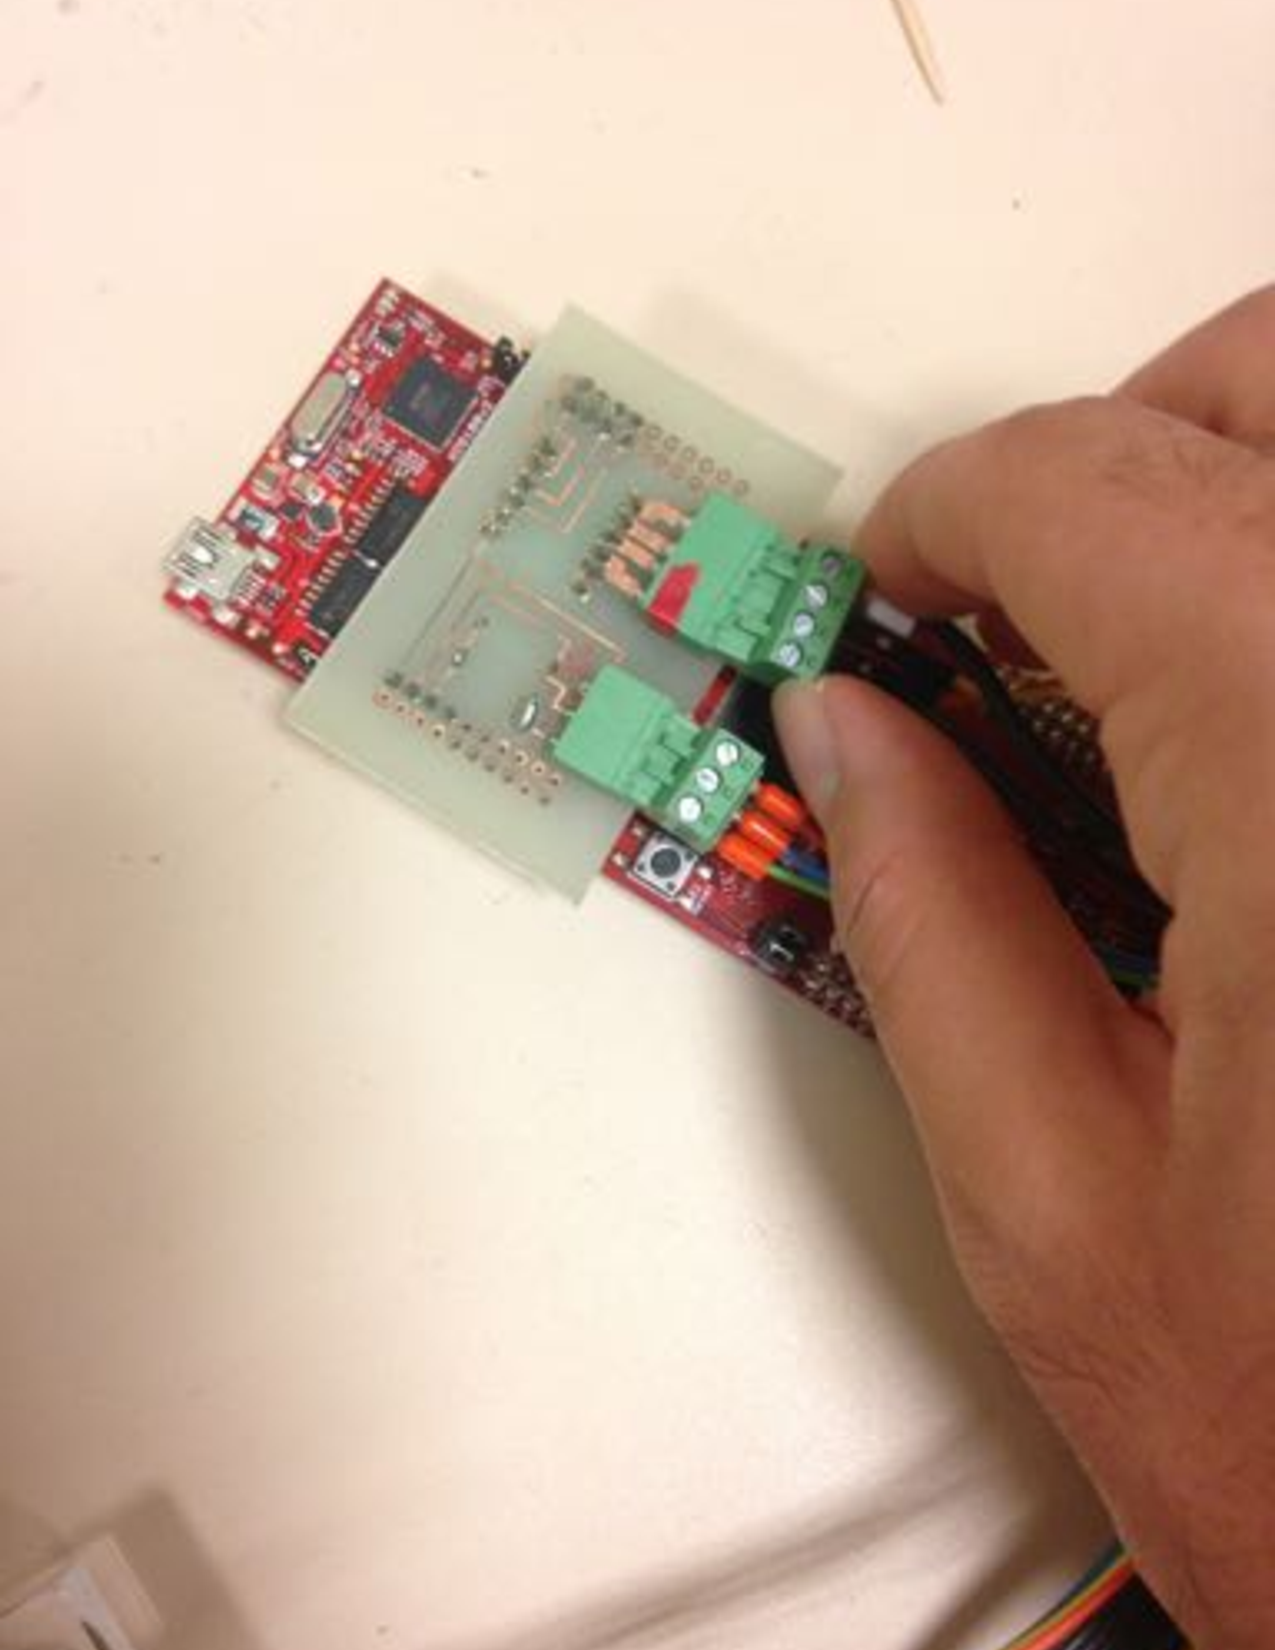
\includegraphics[width=3mm]{./figures/PCB_4pin.pdf}}
\item Plug in both PCB connectors and place the PCB on the microcontroller
\item Plug in the quadrature encoder wires (GND, 5V, A, B) to their corresponding positions on the microcontroller 
\zoombox{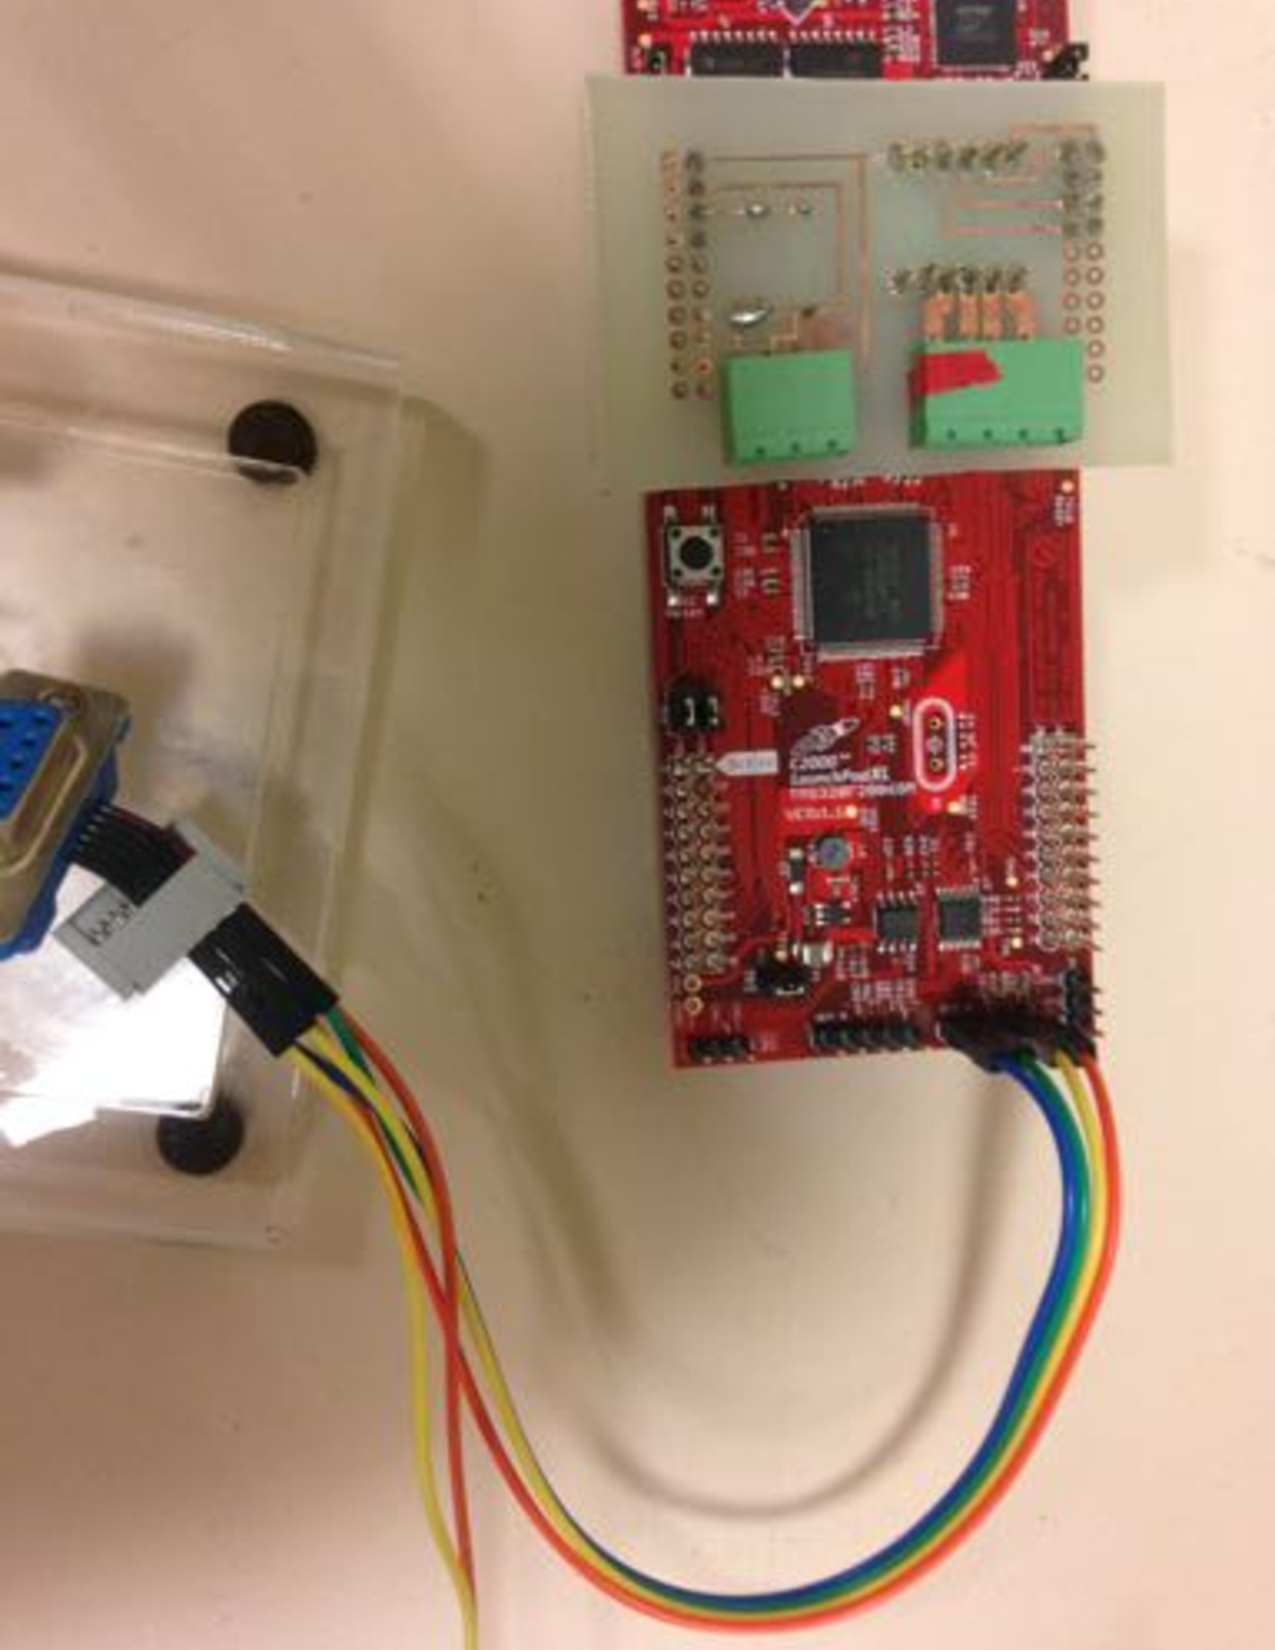
\includegraphics[width=3mm]{./figures/encoder_wiring.pdf}}
\end{enumerate}
The end product of this section should look like 
\zoombox{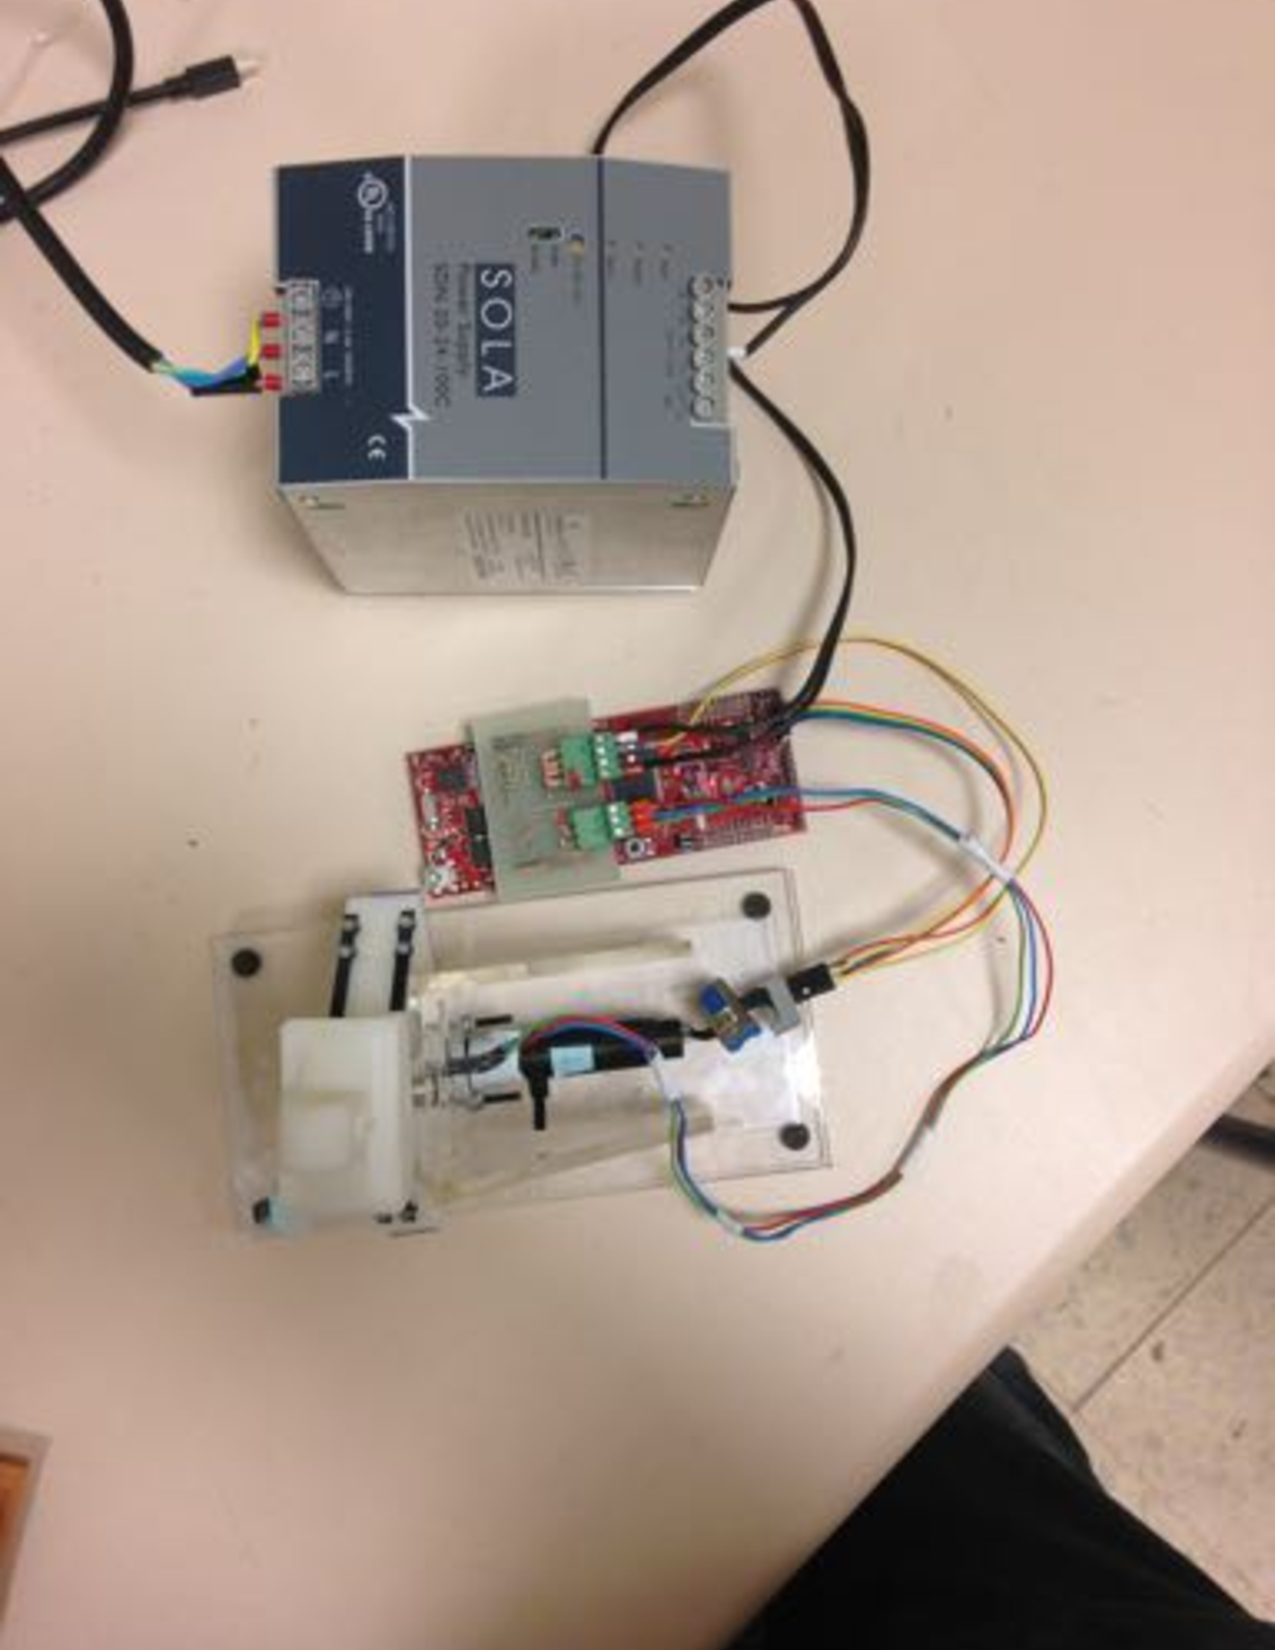
\includegraphics[width=3mm]{./figures/elec_all.pdf}}

\end{itemize}
\end{frame}


\end{document}
